% Copyright (C)  2016  Orestis Malaspinas.
%     Permission is granted to copy, distribute and/or modify this document
%     under the terms of the GNU Free Documentation License, Version 1.3
%     or any later version published by the Free Software Foundation;
%     with no Invariant Sections, no Front-Cover Texts, and no Back-Cover Texts.
%     A copy of the license can be downloaded from:
%     https://www.gnu.org/licenses/fdl.html.

\documentclass[a4paper,12pt]{book}
\usepackage[utf8]{inputenc}
\usepackage[french]{babel}
\usepackage{amsfonts,bm,amsmath,amssymb,graphicx,amsthm}
\usepackage{cancel}
\usepackage{mathtools}

\setlength{\parindent}{0pt}

\newcommand{\real}{\mathbb{R}}
\newcommand{\integer}{\mathbb{Z}}
\renewcommand{\natural}{\mathbb{N}}
\newcommand{\complex}{\mathbb{C}}
\newcommand{\zbar}{\bar{z}}
\newcommand{\dd}{\mathrm{d}}
\newcommand{\perm}{\mathrm{perm}}
\newcommand{\card}{\mathrm{card}}
\newcommand{\fh}{\hat{f}}
\newcommand{\gh}{\hat{g}}
\newcommand{\hh}{\hat{h}}
\renewcommand{\Re}{\mathrm{Re}}
\renewcommand{\Im}{\mathrm{Im}}
\newcommand{\pDeriv}[2]{\frac{\partial #1}{\partial #2}}
\newcommand{\pDerivTwo}[2]{\frac{\partial^2 #1}{\partial #2^2}}
\newcommand{\dDeriv}[2]{\frac{\dd #1}{\dd #2}}
\newcommand{\dDerivTwo}[2]{\frac{\dd^2 #1}{\dd #2^2}}
\newtheorem{definition}{Définition}
\newtheorem*{exemples}{Exemples}
\newtheorem*{exemple}{Exemple}
\newtheorem*{exercice}{Exercice}
\newtheorem*{exercices}{Exercices}
\newtheorem*{remarque}{Remarque}
\newtheorem{proprietes}{Propriétés}
\newtheorem{theoreme}{Théorème}

\title{Résumé du cours de Mathématiques}
\author{Orestis Malaspinas}

\begin{document}
\maketitle

\chapter{Rappel}

\section{Fonctions}
Une fonction $f$ de façon générale est un objet qui prend un (ou plusieurs) paramètres et qui lui (leur) associent un (ou plusieurs) résultats. 
\begin{equation*}
\mbox{résultat}=f(\mbox{paramètres}).
\end{equation*}
\begin{exemples}\hfill\break

\begin{enumerate}
\item La tension $U$ est une fonction de la résistance $R$ et du courant $I$ 
\begin{align}
U=f(R,I)=R\cdot I.
\end{align}
\item Une fonction peut être quelque chose de beaucoup plus général (qu'on ne peut pas forcément représenter simplement avec des opérateurs mathéma-tiques). Prenons le cas de la fonction qui pour un nombre entier $x$ rend le prochain entier qui commence par la même lettre que $x$.
\begin{equation}
f(2)=10,\ f(3)=13,\ ...
\end{equation}
\end{enumerate}
\end{exemples}

Dans ce cours nous allons nous intéresser à des fonctions à un seul paramètre (aussi appelé variable). Si on note la variable $x$ et le résultat $y$, de façon générale on peut écrire 
\begin{equation}
y = f(x).
\end{equation}
Si par ailleurs on a une fonction $g$ et une fonction $f$, on peut effectuer des compositions de fonction, qu'on note $g\circ f$, ou encore 
\begin{equation}
y=g(f(x)).
\end{equation}
\begin{exemples}\hfill\break

\begin{enumerate}
\item Soit $f(x)=2\cdot x$ et $g(x)=\sqrt{x}$, alors la composition des deux fonctions
\begin{equation}
f(g(x))=f(\sqrt{x})=2\sqrt{x}.
\end{equation}
\item On peut composer un nombre arbitraire de fonctions. Voyons le cas avec trois fonctions
$f(x)=2x^2+3$, $g(x)=\cos(2\cdot x)$, et $h(x)=1/x$
\begin{equation}
f(g(h(x)))=f(g(1/x))=f(\cos(2/x))=2\cos^2(2/x)+3.
\end{equation}
\end{enumerate}
\end{exemples}

Pour certaines fonctions, notons les $f(x)$, on peut également définir une fonction inverse
que l'on note $f^{-1}(x)$ dont la composition donne la variable de départ
\begin{equation}
f(f^{-1}(x))=x.
\end{equation}
\begin{exemples}\hfill\break

\begin{enumerate}
\item Soient $f(x)=2\cdot x$ et $f^{-1}(x)=x/2$, alors la composition des deux fonctions
\begin{equation}
f(f^{-1}(x))=f(x/2)=2x/2=x.
\end{equation}
\item Soient $f(x)=x^2$ et $f^{-1}(x)=\sqrt{x}$, alors la composition des deux fonctions
\begin{equation}
f(f^{-1}(x))=f(\sqrt{x})=|x|.
\end{equation}
On a donc que $\sqrt{x}$ est l'inverse de $x^2$ uniquement pour les réels positifs. $f(x)=x^2$ n'a pas d'inverse pour les $x$ négatifs.
\end{enumerate}
\end{exemples}

\section{Domaine de définition}
\noindent
\begin{definition}
 Le domaine de définition, noté $D\subseteq\real$, d'une fonction $f$, est l'ensemble
de valeurs où $f$ admet une image.
\end{definition}

\begin{exemples}\hfill\break
\begin{enumerate}
\item Le domaine de définition de $f(x)=x$ est $D=\real$.
\item Le domaine de définition de $f(x)=1/x$ est $D=\real^\ast$.
\item Le domaine de définition de $f(x)=\sqrt{x+1}/(x-10)$ est $D=[-1;10[\cup]10;\infty[$.
\end{enumerate}
\end{exemples}


\section{Limites}

Soit $f$ une fonction et $D\subseteq\real$ non-vide et non réduit à un point et soient $a$ et $b$ deux réels. 
\subsection{Limite}
\begin{definition}
Pour $f$ définie en $D$, sauf peut-être en $a$, on dit que $b$ est la
limite de $x$ en $a$ si $\lim\limits_{x\rightarrow a}f(x)=b$. C'est-à-dire si on a un
voisinage de $b$ qui contient toutes la valeurs de $f(x)$ pour $x$ proche de $a$.
\end{definition}

\begin{remarque}
Si $f$ est définie en $a$ alors on a $\lim\limits_{x\rightarrow a}=f(a)$.
\end{remarque}

\begin{exemples}
\begin{enumerate}
\item Si $f(x)=x$, alors $\lim\limits_{x\rightarrow 0}f(x)=0$.
\end{enumerate}
\end{exemples}

\begin{definition}
Pour $f$ définie en $D$, sauf peut-être en $a$, et $c$ un réel positif. 
On dit que la limite de $f(x)$ en $a$ tend vers l'infini si
l'intervalle $[c;\infty[$ contient toutes les valeurs de $f(x)$ pour $x$ proche de $a$.
\end{definition}

\begin{exemples}
\begin{enumerate}
\item Si $f(x)=1/x^2$, alors $\lim\limits_{x\rightarrow 0}f(x)=\infty$.
\end{enumerate}
\end{exemples}

\subsection{Limite à gauche, limite à droite}
Pour certaines fonctions, il est possible que le comportement
de celles-ci soit différent selon qu'on approche 
par la gauche ou par la droite (i.e. $f(x)=1/x$). 

On note la limite à droite $\lim\limits{x\rightarrow a^+} f(x)$ ou
$\lim\limits_{x\rightarrow a,x>a} f(x)$ et $\lim\limits{x\rightarrow a^-} f(x)$ ou
$\lim\limits_{x\rightarrow a,x<a} f(x)$ la limite à gauche de la fonction $f$ en $a$.

Si la fonction $f$ admet une limite en $a$, alors les deux limites doivent être égales.

\begin{exemples}
\begin{enumerate}
\item Si $f(x)=1/x$, alors $\lim\limits_{x\rightarrow 0^+} f(x)=\infty$ et $\lim\limits_{x\rightarrow 0^-} f(x)=-\infty$.
\end{enumerate}
\end{exemples}

\subsection{Asymptotes}

Dans certains cas il peut être intéressant d'étudier le comportement des fonctions quand $x\rightarrow\pm\infty$. 
Dans ces cas-là on dit qu'on s'intéresse au comportement \textit{asymptotique} d'une fonction. Ce concept est particulièrement
relevant quand on étudie une fonction que a la forme d'une fraction
\begin{equation}
 h(x)=\frac{f(x)}{g(x)}.
\end{equation}
Si on s'intéresse au comportement à l'infini de cette fonction on va prendre sa ``limite'' lorsque $x\rightarrow\infty$
\begin{equation}
 \lim_{x\rightarrow\infty} h(x)=\lim_{x\rightarrow\infty}\left(\frac{f(x)}{g(x)}\right).
\end{equation}
Un exemple peut être $f(x)=x-1$, $g(x)=x+1$ et donc $h(x)=(x-1)/(x+1)$
\begin{equation}
 \lim_{x\rightarrow\infty} \frac{x-1}{x+1}=\lim_{x\rightarrow\infty} \frac{x}{x}=1.
\end{equation}
De même quand on a $f(x)=3x^4-5x^3+1$, $g(x)=1$ et donc $h(x)=3x^4-5x^3+1$. Il vient donc
\begin{equation}
 \lim_{x\rightarrow\infty} 3x^4-5x^3+1=\lim_{x\rightarrow\infty}3x^4=\infty.
\end{equation}

Si nous compliquons un peu l'exemple, et que nous avons $f(x)=x^3+3x^2+1$, $g(x)=x^2$ et donc $h(x)=(x^3+3x^2+1)/x^2$
\begin{equation}
 \lim_{x\rightarrow\infty} (x^3+3x^2+1)/x^2=\lim_{x\rightarrow\infty} x=\infty.
\end{equation}
Ce genre d'estimations est imporant en informatique lors de l'analyse de performance des algorithmes.
On peut prendre l'exemple des algorithmes de tri ``bubble sort'' et ``quick sort''. Leur complexité 
respective moyenne est de $n^2$ et de $n\log(n)$, quand $n$ est le nombre d'éléments de la chaîne à trier.
Si on fait le rapport pour de ces deux complexités on a 
\begin{equation}
 \lim_{n\rightarrow\infty} \frac{n^2}{n\log(n)}=\lim_{n\rightarrow\infty} \frac{n}{\log(n)}.
\end{equation}
On peut simplement voir que ce rapport va tendre vers l'infini en dessinant la courbe $n/\log(n)$. 
Il existe un moyen ``analytique'' d'évaluerce rapport. Tout nombre $n$ peut s'écrire avec une précision $p$ comme
\begin{equation}
 n=A\cdot 10^{p-1},
\end{equation}
où $p$ est le nombre de chiffres significatifs qu'on veut représenter, et $1\leq A< 10$. On a également que\footnote{Pour ceux que ça intéresse 
cette série s'obtient à l'aide d'une série de Taylor.}
\begin{equation}
 \log(A)=\log\left(\frac{1+y}{1-y}\right)=2\sum_{k=0}^\infty \frac{y^{2k+1}}{2k+1},
\end{equation}
avec $y=(A-1)/(A+1)$. On a finalement que
\begin{equation}
 \log(n)=\log(A\cdot 10^{p-1})=(p-1)\log(10)+2\sum_{k=0}^\infty \frac{y^{2k+1}}{2k+1}.
\end{equation}
La valeur de $y$ étant quelque chose de proche de 0, la somme converge vite vers une valeurs finie et on peut faire l'approximation
\begin{equation}
 \log(n)\cong(p-1)\log(10),
\end{equation}
pour $n$ grand (ce qui est équivalent à $p$ grand).
On a donc que finalement le rapport $n/\log(n)$ va comme
\begin{equation}
 \lim_{n\rightarrow\infty}\frac{n}{\log(n)}=\frac{A}{\log(10)}\cdot\lim_{n\rightarrow\infty}\frac{10^{p-1}}{(p-1)}=\frac{A}{\log(10)}\cdot\lim_{n\rightarrow\infty}\frac{10^{p-1}}{p}=\infty.
\end{equation}



\section{Continuité}

\begin{definition} 
Soit $f$ une fonction définie sur un intervalle ouvert $D$ contenant $a$. 
On dit que $f$ est continue en $a$ si et seulement si $\lim\limits_{x\rightarrow a}f(x)=f(a)$.
\end{definition}

\begin{proprietes} 
Soient $f$ et $g$ deux fonctions continues en $a$ alors et $b$ un réel:
\begin{enumerate}
\item $f+g$ est continue en $a$.
\item $b f$ est continue en $a$.
\item si $g(a)\neq 0$, $f/g$ est continue en $a$.
\item $h=g\circ f$ est continue en $a$.
\end{enumerate}
\end{proprietes}

\begin{definition} 
Une fonction $f$ est dite continue dans un intervalle $D=]a;b[$ 
si et seulement si elle est continue en tout point de $D$. De plus, elle est 
continue sur $D=[a,b]$ si elle est continue sur $]a;b[$ et continue à droite en $a$
et à gauche en $b$.
\end{definition}

\begin{theoreme} [Théorème des valeurs intermédiaires]
Soit $f$ une fonction continue sur $D$, et $a,b$ deux points contenus dans $D$ tels que $a<b$ et $f(a)<f(b)$, alors 
\begin{equation}
\forall y\in [f(a);f(b)],\ \exists\ c|f(c)=y.
\end{equation}
\end{theoreme}
 

\section{Dérivées}

\begin{definition} Soit $f$ une fonction définie sur $D$ et $a\in D$. On dit que 
$f$ est dérivable en $a$ s'il existe un $b$ (appelé la dérivée de $f$ en $a$) tel que
\begin{align}
&\lim\limits_{h\rightarrow 0}\frac{f(a+h)-f(a)}{h}=b,\hbox{ ou}\\
&\lim\limits_{x\rightarrow a}\frac{f(x)-f(a)}{x-a}=b.
\end{align}
\end{definition}

\begin{definition} Si $f$ est dérivable en tout point de $D=]a;b[$, alors on définit
$f'$ la fonction dérivée de $f$ dans l'intervalle $D$ qui associe en tout point $x$ de
$D$ la valeur dérivée de $f$.
\end{definition}

\begin{proprietes} 
Si $f$ est dérivable en $a$ alors $f$ est continue en $a$. 
\end{proprietes}

\begin{proprietes} 
Soient $f$ et $g$ deux fonctions dérivables (dont les dérivées sont $f'$ et $g'$), et $a\in\real$, alors
\begin{enumerate}
\item $(f+g)'=f'+g'$.
\item $(af)'=a f'$.
\item $(f\cdot g)'=f'g+fg'$.
\item Si $g$ ne s'annule pas $(f/g)'=(f'g-fg')/g^2$.
\item $(g\circ f)'=(g'\circ f)\cdot f'$.
\end{enumerate}
\end{proprietes}

Il existe quelques dérivées importantes que nous allons utiliser régulièrement dans la suite de ce cours. 
En supposons que $C\in \real$, nous avons
\begin{enumerate}
\item $f(x)=x^n$, $f'(x)=nx^{n-1}$ .
\item $f(x)=e^{C x}$, $f'(x)=Ce^{Cx}$.
\item $f(x)=\ln(x)$, $f'(x)=\frac{1}{x}$.
\item $f(x)=C, $f'(x)=0.
\item $f(x)=\sin(x)$, $f'(x)=\cos(x)$.
\item $f(x)=\cos(x)$, $f'(x)=-\sin(x$).
\end{enumerate}


\begin{definition} 
Si $f'$ est dérivable sur $D$, alors sa dérivée, notée $f''$, est appelée la dérivée seconde de $f$.
\end{definition}

\subsection{Variation des fonctions}

\begin{proprietes} Soit $f'$ la fonction dérivée de $f$ sur $D$
\begin{enumerate}
\item Si $f'>0$ sur $D$, alors $f$ est croissante sur $D$.
\item Si $f'<0$ sur $D$, alors $f$ est décroissante sur $D$.
\item Si $f'=0$ sur $D$, alors $f$ est constante sur $D$.
\end{enumerate}
\end{proprietes}

\begin{definition} 
Une fonction admet un maximum local (respectivement minimum local) 
sur un intervalle $D=]a;b[$ s'il existe un $x_0$ tel que $f(x_0)\geq f(x)$ (respectivement $f(x_0)\leq f(x)$) pour tout $x\in D$. 
\end{definition}

\begin{proprietes}
Soit $f$ une fonction dérivable sur $D=]a;b[$ et $x_0\in D$. Si $f$ admet
un maximum ou un minimum en $x_0$ alors $f'(x_0)=0$. De plus si 
$f'(x_0)=0$ et $f'$ change de signe en $x_0$ alors $f(x_0)$ est un maximum ou un minimum de $f$.
\end{proprietes}

\section{Etude de fonction}

Effectuer l'étude de fonction de la fonction suivante 
\begin{equation}
 f(x)=\frac{x^3}{x^2-4}.
\end{equation}
\begin{enumerate}
 \item Déterminer le domaine de définition.
 \item Déterminer la parité de la fonction. Rappel:
 \begin{align}
  f(-x)&=f(x),\ \mbox{paire},\\
  f(-x)&=-f(x),\ \mbox{impaire}.
 \end{align}
 \item Trouver les zéros de la fonction (Indication: trouver les $x$ tels que $f(x)=0$).
 \item Trouver les éventuelles asymptotes verticales ou disconsinuités, ainsi que les asymptotes affines.
 \item Caluler $f'(x)$ et déterminer sa croissance et points critiques (déterminer où la fonction est croissante, décroissante, atteint un extremum, etc).
 \item Faire un croquis de $f(x)$.
\end{enumerate}



\chapter{Intégrales}

\section{Interprétation géométrique}
Dans ce chapitre nous nous intéressons au calcul d'aires sous une fonction $f$.
La fonction $f$ satisfait les hypothèses suivantes. 
\begin{enumerate}
\item $f(x)$ est bornée dans l'intervalle $[a,b]\in\real$. 
\item $f(x)$ est continue presque partout.
\end{enumerate}

Nous définissions également l'infimum de $f$ sur un intervalle $[x_0,x_1]$, noté 
\begin{equation*}
\inf\limits_{[x_0,x_1]} f(x)
\end{equation*}
comme étant la valeur bornant par dessous toutes les valeurs prises par $f(x)$ dans l'intervalle $[x_0,x_1]$. Le suprémum sur un intervalle $[x_0,x_1]$, noté 
\begin{equation*}
\sup\limits_{[x_0,x_1]} f(x)
\end{equation*}
comme étant la valeur bornant par dessus toutes les valeurs prises par $f(x)$ dans l'intervalle $[x_0,x_1]$.

Finalement nous définissons une subdivision 
\begin{equation*}
\Delta_n=\{a=x_0<x_1<...<x_{n-1}<x_{n}=b\}
\end{equation*}
est une suite finie contenant $n$ termes dans $[a,b]$. 

On peut à présent approximer l'aire sous la fonction $f(x)$ dans l'intervalle $[a,b]$ 
de deux façon:
\begin{enumerate}
\item $A^i(n)=\sum_{i=0}^{n-1} \inf\limits_{[x_i,x_{i+1}]} f(x) (x_{i+1}-x_i)$ comme étant l'aire inférieure.
\item $A^s(n)=\sum_{i=0}^{n-1} \sup\limits_{[x_i,x_{i+1}]} f(x) (x_{i+1}-x_i)$ comme étant l'aire supérieure.
\end{enumerate}
L'aire de sous la fonction $f(x)$ est donnée par la limite pour $n\rightarrow\infty$ 
de $A^i$ ou $A^s$ (si elle existe).
\begin{remarque}\hfill\break
\begin{enumerate}
\item Ces sommes peuvent être positives ou négatives en fonction du signe de $f$.
\item Une implantation informatique est immédiate.
\end{enumerate}
\end{remarque}

\begin{definition}[Intégrabilité au sens de Riemann]
Une fonction est dite intégrable au sens de Riemann si 
$\lim\limits_{n\rightarrow\infty}A^i(n)=\lim\limits_{n\rightarrow\infty}A^s(n)=\int_a^b f(x)\dd x$.
\end{definition}
Dans la formule $\int_a^b f(x)\dd x$ Ici $x$ est appelée variable d'intégration, 
$a$ et $b$ sont les bornes d'intégration. Pour des raisons de consistance dans les notations la variable d'intégration ne peut être désignée avec le même symbole qu'une des bornes d'intégration. 

\begin{exemples}Intégration de $f(x)=x$ dans intervalle $[0,1]$.

Il est trivial de calculer 
que cette aire vaut $1/2$ (c'est l'aire d'un triangle rectangle de côté 1). Néanmoins, évaluons également cette aire à l'aide de $A^i$ et $A^s$. Commençons par subdiviser $[0,1]$ en $n$ intervalles égaux de longueur 
$\delta=1/n$. Comme $f(x)$ est strictement croissante, on a que 
$\inf\limits_{[x_i,x_{i+1}]}f(x)=f(x_i)$ et que $\sup\limits_{[x_i,x_{i+1}]}f(x)=f(x_{i+1})$. On a donc que
\begin{enumerate}
\item $A^i(n)=\delta\sum_{i=0}^{n-1} x_i=\delta\sum_{i=0}^{n-1}\frac{i}{n}=\frac{n(n-1)}{2n^2}=\frac{n-1}{2n}$\footnote{
La somme $\sum_{i=0}^n i=n(n+1)/2$}. Et donc en prenant la limite pour $n\rightarrow\infty$ il vient
\begin{equation}
A^i=\lim\limits_{n\rightarrow\infty}\frac{n-1}{2n}=\frac{1}{2}.
\end{equation}

\item $A^s(n)=\delta\sum_{i=0}^{n-1} x_i=\delta\sum_{i=0}^{n-1}\frac{i+1}{n}=\delta\sum_{i=0}^{n}\frac{i}{n}=\frac{n(n+1)}{2n^2}=\frac{n+1}{2n}$. Et donc en prenant la limite pour $n\rightarrow\infty$ il vient
\begin{equation}
A^s=\lim\limits_{n\rightarrow\infty}\frac{n+1}{2n}=\frac{1}{2}.
\end{equation}

\end{enumerate}

\end{exemples}

\begin{exercice}
Calculer l'aire sous la courbe de $f(x)=x^2$ dans intervalle $[0,1]$.

Indication: $\sum_{i=0}^n i^2=\frac{1}{6}n(n+1)(2n+1).$
\end{exercice}

\section{Interprétation physique}

Supposons que nous ayons une fonction, $x(t)$, qui donne la position d'un objet pour un intervalle 
de temps $t\in[a,b]$. Nous pouvons aisément en déduire la vitesse $v(t)$ de l'objet, comme étant la variation
de $x(t)$ pour tout $t$. Autrement dit $v(t)=x'(t)$.

Supposons à présent que nous ne connaissions que la vitesse $v(t)$ de notre objet. Afin de déduire sa position
nous prendrions un certain nombre d'intervalles de temps $\delta t_i=t_{i+1}-t_i$ que nous multiplierions
par $v(t_i)$ afin de retrouver la distance parcourue pendant l'intervalle $\delta t_i$
et ainsi de suite. Afin d'améliorer l'approximation de la distance parcourue 
nous diminuerions la valeur de $\delta t_i$ jusqu'à ce que $\delta t_i\rightarrow 0$.

Nous voyons donc que cette méthode, n'est autre qu'une façon ``intuitive'' d'intégrer la vitesse afin de trouver la position.
Et que donc l'intégrale et la dérivée sont étroitement liée. La vitesse étant la dérivée de la position et la position étant l'intégrale de la vitesse.


\section{Primitive}
Si maintenant nous essayons de généraliser le calcul de l'intégrale d'une fonction,
il s'avère que le calcul d'une intégrale est l'inverse du calcul d'une dérivée.

\begin{definition}[Primitive]
Soit $f$ une fonction. On dit que $F$ est la primitive de $f$ sur l'intervalle $D\subseteq\real$ si $F'(x)=f(x)$  $\forall x\in D$.
\end{definition}

Si $F$ est une primitive de $f$, alors on peut définir la fonction $G$ telle que $G(x)=F(x)+C$, $\forall C\in\real$ 
qui est aussi une primitive de $f$. On dit donc que la primitive de $f$ est définie à une constante additive près. En effet,
si $F'=f$ on a
\begin{equation}
 G'=F'+\underbrace{C'}_{=0}=F'=f.
\end{equation}
\begin{theoreme}[Unicité]
S'il existe $a\in D$ et $b\in\real$ alors il existe une unique primitive
$F$ telle que $F(a)=b$.
\end{theoreme}
\begin{exemple}
 Soit $f(x)=x$, alors l'ensemble de primitives correspondantes est $G=x^2/2+C$. Si nous cherchons la 
 primitive telle que $G(0)=0$, il vient que $C=0$ et donc la primitive est unique et vaut
 $F(x)=x^2/2$.
\end{exemple}
\begin{exercices}
Calculez les primitives suivantes (\textit{Indication: Il s'agit de trouver les fonctions $F(x)$ telles que $F'(x)=f(x)$}):
 \begin{enumerate}
  \item $f(x)=\int x^2\dd x$.
  \item $f(x)=\int x^n\dd x$, $n\in \real\backslash\{-1\}$.
  \item $f(x)=\int \sqrt{x}\dd x$.
  \item $f(x)=\int \frac{1}{x}\dd x$.
  \item $f(x)=\int \exp(x)\dd x$.
  \item $f(x)=\int \sin(x)\dd x$.
 \end{enumerate}
\end{exercices}

Maintenant que vous avez calculé toutes ces primitives de base, nous pouvons récapituler 
des formules qui seront importantes pour la suite:
 \begin{enumerate}
  \item $\int x^n\dd x=\frac{1}{n+1}x^{n+1}+C$, $n\in \real\backslash\{-1\}$.
  \item $\int \frac{1}{x}\dd x=\ln(x)+C$.
  \item $\int \exp(x)\dd x=\exp(x)+C$.
  \item $\int \sin(x)\dd x=-\cos(x)+C$.
  \item $\int \cos(x)\dd x=\sin(x)+C$.
 \end{enumerate}

\begin{definition}\label{def_prim}
En définissant à présent l'intégrale à l'aide de la notion de primitive, nous avons
que pour $a,b\in\real$ et $a<b$
\begin{equation}
 \int_a^b f(x)\dd x=\left.F\right|_a^b=F(b)-F(a).
\end{equation}
\end{definition}
On dit que $x$ est la variable d'intégration. Elle est dite ``muette'' car elle disparaît après que l'intégrale ait été effectuée.
On peut donc écrire l'équation ci-dessus de façon équivalente en remplaçant le symbole $x$ par n'importe quelle autre lettre (sauf $a,b,f,F$).
\begin{remarque}
 On notera que la constante additive $C$ a disparu de cette formule. En effet, remplaçons $F$ par $G=F+C$, il vient
\begin{equation*}
 \int_a^b f(x)\dd x=G(b)-G(a)=F(b)+C-F(a)-C=F(b)-F(a). 
\end{equation*}
\end{remarque}
De la définition \ref{def_prim}, il vient immédiatement que 
\begin{equation}
 \int_a^af(x)\dd x=F(a)-F(a)=0
\end{equation}
et que
\begin{equation}
 \int_a^bf(x)\dd x= -\int_b^af(x)\dd x
\end{equation}

Nous pouvons à présent définir la fonction $G(x)$ telle que
\begin{equation}
 G(x)=\int_a^xf(y)\dd y=F(x)-F(a).
\end{equation}
Nous avons donc que $G(x)$ est la primitive de $f$ telle que $G(a)=0$.


\begin{proprietes}
Soient $f$ et $g$ deux fonctions intégrables sur un intervalle $D=[a,b]\subseteq\real$, $c\in[a,b]$, et $\alpha\in\real$.
On a
\begin{enumerate}
 \item La dérivée et l'intégrale ``s'annulent'' 
 \begin{equation}
  \left[\int_a^x f(y)\dd y\right]'=f(x), \quad x\in D.
 \end{equation}
 \item La fonction $h=f+g$ admet aussi une primitive sur $D$, et on a
 \begin{equation}
  \int_a^b(f(x)+g(x))\dd x=\int_a^b f(x)\dd x+\int_a^b g(x)\dd x.
 \end{equation}
 \item La fonction $h=\alpha f$ admet aussi une primitive sur $D$, et on a
 \begin{equation}
  \int_a^b\alpha f(x)\dd x=\alpha\int_a^b f(x)\dd x.
 \end{equation}
\item Relation de Chasles (faire la démonstration en exercice)
\begin{equation}
\int_a^c f(x)\dd x=\int_a^b f(x)\dd x+\int_b^c f(x)\dd x.
\end{equation}
De cette relation on déduit qu'on peut calculer l'intégrale d'une fonction
continue par morceaux sur $[a,b]$.
\item Si $f$ est paire alors
\begin{equation}
\int_{-a}^a f(x)\dd x = 2\int_0^a f(x)\dd x.
\end{equation}
\item Si $f$ est impaire alors
\begin{equation}
\int_{-a}^a f(x)\dd x = 0.
\end{equation}
\end{enumerate}
\end{proprietes}



\subsection{Intégrales impropres}

Si une des bornes d'intégration ou si la fonction à intégrer admet une discontinuité à des points bien définis, nous
parlons intégrales impropres.

Lorsqu'une borne d'intégration est infinie, alors nous pouvons avoir les cas de figures suivants
\begin{align}
 &\int_a^\infty f(x)\dd x=\lim\limits_{b\rightarrow\infty}\int_a^b f(x)\dd x,\\
 &\int_{-\infty}^b f(x)\dd x=\lim\limits_{a\rightarrow\infty}\int_{-a}^b f(x)\dd x,\\
 &\int_{-\infty}^\infty f(x)\dd x=\lim\limits_{a\rightarrow\infty}\int_{-a}^a f(x)\dd x.
\end{align}
\begin{exemple}
Calculer l'intégrale suivante
\begin{equation}
\int_0^\infty e^{-ax}\dd x,\quad a>0.
\end{equation}
Nous pouvons réécrire l'intégrale ci-dessus comme
\begin{equation*}
\int_0^\infty e^{-ax}\dd x=\lim\limits_{b\rightarrow \infty}\int_0^b e^{-ax}\dd x=-\frac{1}{a}\lim\limits_{b\rightarrow\infty}\left[e^{-ax}\right]_0^b=-\frac{1}{a}\left[\lim\limits_{b\rightarrow \infty}e^{-ab}-1\right]=\frac{1}{a}.
\end{equation*}
\end{exemple}
\begin{exercice}
 Calculer l'intégrale suivante
\begin{equation}
\int_1^\infty \frac{1}{x^2}\dd x.
\end{equation}
\end{exercice}

Lorsque nous avons une discontinuité dans la fonction $f$ au point $c\in[a,b]$ nous avons
\begin{equation}
 \int_a^b f(x)\dd x = \lim\limits_{\varepsilon\rightarrow 0}\int_a^{c-\varepsilon} f(x)\dd x +\int_{c+\varepsilon}^b f(x)\dd x.
\end{equation}
\begin{exercice}
 Montrer que 
\begin{equation}
 \int_{-1}^2\frac{1}{x}=\ln{2}.
\end{equation}

\end{exercice}




\begin{definition}[Valeur moyenne]
Soit une fonction $f$ admettant une primitive sur $[a,b]$ et $a<b$, alors on appelle
la valeur moyenne de cette fonction sur $[a,b]$, $\bar{f}$, 
\begin{equation}
\bar{f}=\frac{1}{b-a}\int_a^bf(x)\dd x.
\end{equation}

\end{definition}



\section{Méthodes d'intégration}
Dans cette section, nous allons étudier différentes méthodes pour intégrer des fonctions.

\subsection{Intégration de fonctions usuelles et cas particuliers}
Le calcul d'une primitive ou d'une intégrale n'est en général pas une chose aisée. Nous connaissons les formules d'intégration
pour certaines fonctions particulières.
\subsubsection{Polynômes}
Les polynômes s'intègrent terme à terme. Pour $\{a_i\}_{i=0}^{n}\in\real$
\begin{align}
 &\int a_0 + a_1 x + a_2 x^2+\cdots+a_{n-1} x^{n-1}+a_{n} x^{n}\dd x\\
 =&\int a_0\dd x + \int a_1 x\dd x + \int a_2 x^2\dd x+\cdots+\int a_{n-1} x^{n-1}\dd x+\int a_{n} x^{n}\dd x\\
 =&a_0 x + \frac{a_1}{2}x^2+\frac{a_2}{3}x^3+\cdots+\frac{a_n}{n+1}x^{n+1}+c.
\end{align}
\begin{exercice}
 Intégrer la fonction suivante
 \begin{equation}
  \int (x+2)(x^3+3x^2+4x-3)\dd x.
 \end{equation}
\end{exercice}
\subsubsection{Application de la règle de chaîne pour l'intégration}
Une primitive de la forme
\begin{equation}
 \int f(x)f'(x)\dd x=\frac{1}{2}f(x)^2+c.
\end{equation}
\begin{exemple}
 Le calcul de la primitive suivante 
\begin{equation}
 \int \sin(x)\cos(x)\dd x=\frac{1}{2}\sin^2(x)+c.
\end{equation} 
\end{exemple}

\subsubsection{Inverse de la dérivation logarithmique}
Une primitive de la forme
\begin{equation}
 \int \frac{f'(x)}{f(x)}\dd x=\ln(f(x))+c.
\end{equation}
\begin{exemple}[Trivial]
 Le calcul de la primitive de suivante 
\begin{equation}
 \int \frac{1}{x}\dd x=\int \frac{(x)'}{x}\dd x=\ln(x)+c.
\end{equation} 
\end{exemple}

\subsubsection{Règle de chaîne}
De façon une des façons les plus simples de calculer une primitive est de reconnaître la règle de chaîne 
dans le terme à intégrer
\begin{equation}
 \int g'(f(x))f'(x)\dd x=\int [g(f(x))]' \dd x=g(f(x))+c.
\end{equation}
\begin{exemple}
Si $g$ est définie comme $g(x)=x^{-1}$ et $f(x)=3x^2+2$, alors la primitive 
\begin{equation}
 \int \frac{f'(x)}{g'(f(x))}\dd x=\int -\frac{6 x}{(3x^2+2)^2}\dd x=\frac{1}{3x^2+2}.
\end{equation} 
\end{exemple}




\subsection{Intégration par parties}
La dérivation d'un produit de fonction $f\cdot g$ s'écrit
\begin{equation}
 (f(x)g(x))'=f'(x) g(x)+f(x) g'(x).
\end{equation}
En intégrant cette équation on obtient
\begin{equation}
 f(x)g(x)=\int f'(x) g(x)\dd x+\int f(x) g'(x)\dd x.
\end{equation}
Une primitive de la forme $\int f'(x) g(x)\dd x$ peut se calculer de la façon suivante
\begin{equation}
 \int f'(x) g(x)\dd x=f(x)g(x)-\int f(x) g'(x)\dd x.
\end{equation}
De façon similaire si nous nous intéressons à une intégrale définie
\begin{equation}
 \int_a^b f'(x) g(x)\dd x=\left.(f(x)g(x))\right|_a^b-\int_a^b f(x) g'(x)\dd x.
\end{equation}
Le choix des fonctions est complètement arbitraire. 
Néanmoins, le but de cette transformation est de remplacer une intégrale par une autre dont on connaîtrait la solution.

Des ``règles'' pour utiliser cette technique seraient que 
\begin{enumerate}
\item $g'$ soit facile à calculer et aurait une forme plus simple que $g$.
\item $f=\int f'\dd x$ soit facile à calculer et aurait une forme plus simple que $f'$.
\end{enumerate}
\begin{exemples}
Calculer les primitives suivantes
 \begin{enumerate}
  \item $\int x e^x\dd x$. $g(x)=x$, $f'(x)=e^x$ et donc $g'(x)=1$, $f(x)=e^x$. Il vient
  \begin{equation}
    \int x e^x=x e^x-\int e^x\dd x=x e^x-e^x+c.
  \end{equation}
  \item $\int \cos(x)\sin(x)\dd x$. $g= \cos(x)$, $f'(x)=\sin(x)$ et donc $g'(x)=-\sin(x)$, $f(x)=-\cos(x)$. Il vient
  \begin{align}
    &\int \cos(x)\sin(x)\dd x=\sin^2(x)-\int \cos(x)\sin(x)\dd x\nonumber\\
    \Rightarrow &\int \cos(x)\sin(x)\dd x=\frac{1}{2}\sin^2(x).
  \end{align}
  On voit que le résultat de l'intégration par partie nous redonne l'intégrale de départ. Ceci nous permet d'évaluer directement la dite intégrale.
 \end{enumerate}

\end{exemples}
Il est également possible d'enchaîner plusieurs intégrations par parties.
\begin{exemple}
L'intégrale de $\int x^2 e^x\dd x$. En posant $g(x)=x^2$, $f'(x)=e^x$ et donc $g'(x)=2x$, $f(x)=e^x$. Il vient
\begin{equation}
 \int x^2 e^x\dd x=x^2e^x-2\int x e^x\dd x.
\end{equation}
On pose de façon similaire $g(x)=x$, $f'(x)=e^x$ et donc $g'(x)=1$, $f(x)=e^x$ et il vient
\begin{equation}
\int x^2 e^x\dd x=x^2e^x-2\left(x e^x -\int e^x\dd x\right)=x^2e^x-2x e^x +2e^x+c.
\end{equation}
\end{exemple}

\begin{exercices}
Calculer les primitives suivantes
\begin{enumerate}
 \item $\int \ln(x)\dd x$
 \item $\int x^2 \sin(x)\dd x$
 \item $\int e^x\sin(x)\dd x$
\end{enumerate}

\end{exercices}


\subsection{Intégration par changement de variables}

On observe que la dérivation de la composition de deux fonctions $F$ et $g$ est donnée par
\begin{equation}
 (F\circ g)'=(f\circ g)\cdot g',\mbox{ ou } [F(g(y))]'=f(g(y))\cdot g'(y),
\end{equation}
où $f=F'$. Si nous intégrons cette relation on obtient
\begin{align*}
 \int_a^b f(g(y))g'(y)\dd y = \int_a^b [F(g(y))]'\dd y=\left.F(g(y))\right|_a^b=F(g(b))-F(g(a))=\int_{g(a)}^{g(b)}f(x)\dd x.
\end{align*}
Cette relation nous mène au théorème suivant.
\begin{theoreme}[Intégration par changement de variables]
Soit $f$ une fonction continue presque partout, et $g$ une fonction dont la dérivée est continue presque partout sur un intervalle 
$[a,b]$. Soit également l'image de $g$ contenue dans le domaine de définition de $f$. Alors
\begin{equation}
 \int_a^b f(g(x))g'(x)\dd x = \int_{g(a)}^{g(b)}f(z)\dd z.
\end{equation}
\end{theoreme}
Nous utilisons ce théorème de la façon suivante. L'idée est de remplacer la fonction $g(x)$ par $z$. Puis il faut également
remplacer $\dd x$ par $\dd z$ où nous avons que $\dd x=\dd z/g'(x)$. Finalement, il faut changer les bornes d'intégration 
par $a\rightarrow g(a)$ et $b\rightarrow g(b)$. Si on ne calcule pas l'intégrale mais la primitive, on ne modifie (évidemment) pas
les bornes d'intégration, mais en revanche pour trouver la primitive il faut également appliquer la transformation
$x=g^{-1}(z)$ sur la solution.
\begin{exemple}
 Intégrer par changement de variables $\int_1^3 6x\ln(x^2)\dd x$.
 
 En définissant $z=x^2$, nous avons $\dd x=\dd z/(2x)$. Les bornes d'intégration deviennent $z(1)=1^2=1$ et $z(3)=3^2=9$.
 On obtient donc
 \begin{align*}
  \int_1^3 6x\ln(x^2)\dd x&=\int_1^9 6x\ln(z)\frac{1}{2x}\dd z=\int_1^9\ln(z)\dd z\nonumber\\
                          &=3\left[z\ln(z)-z\right]_1^9=3(9\ln(9)-9-\ln(1)+1)=27\ln(9)-24.
 \end{align*}

\end{exemple}
\begin{exercices}
Calculer les primitives suivantes par changement de variable
 \begin{enumerate}
  \item $\int \frac{1}{5x-7}\dd x$
  \item $\int \sin(3-7x)\dd x$
  \item $\int x e^{x^2}\dd x$
 \end{enumerate}

\end{exercices}





\section{Intégration numérique}

Dans certains cas, il est impossible d'évaluer analytiquement une intégrale ou alors elle est très compliquée à calculer.
Dans ce cas, on va approximer l'intégrale et donc commettre une erreur.

Pour ce faire on va subdiviser l'espace d'intégration $[a,b]$ en $N$ pas équidistants (pour simplifier) $\delta x=(b-a)/N$,
et approximer l'intégrale par une somme finie
\begin{equation}
 \int_a^bf(x)\dd x=\sum_{i=0}^{N} \delta x f(a+i\delta x) g_i+E(a,b,\delta x)\cong\sum_{i=0}^{N} \delta x f(a+i\delta x) g_i,
\end{equation}
où $g_i$ est un coefficient qui va dépendre de la méthode d'intégration 
que nous allons utiliser, $E$ est l'erreur commise par l'intégration numérique et va dépendre des bornes d'intégration, 
de $\delta x$ (du nombre de pas d'intégration), de la forme de $f(x)$ (combien est ``gentille'') et finalement de
la méthode d'intégration.

\subsection{Erreur d'une méthode d'intégration}

D'une façon générale plus $\delta x$ est petit ($N$ est grand) plus l'erreur sera petite et donc l'intégration sera précise
(et plus le calcul sera long).
Néanmoins, comme la précision des machines sur lesquelles nous évaluons les intégrale est finie, si $\delta x$ devient 
proche de la précision de la machine des erreurs d'arrondi vont dégrader dramatiquement la précision de l'intégration.

\begin{remarque}
De façon générale il est difficile de connaître à l'avance la valeur exacte de $E$. En revanche on est
en capable de déterminer \textbf{l'ordre} de l'erreur.
\end{remarque}

\begin{definition}[Ordre d'une méthode]
 On dit qu'une méthode d'intégration est d'ordre $k$, si l'erreur commise par la méthode varie 
 proportionnellement à $\delta x^k$. On note qu'une erreur est d'ordre $k$ par le symbole $\mathcal{O}(\delta x^k)$. Exemple: si une méthode est d'ordre deux, alors en diminuant 
 $\delta x$ d'un facteur $2$, l'erreur sera elle divisée par $2^2=4$. Si une méthode est d'ordre $3$, alors en diminuant 
 $\delta x$ d'un facteur $2$, nous aurons que l'erreur est divisée par un facteur $2^3=8$. Etc.
\end{definition}

Comme le calcul d'une intégrale de façon numérique ne donne en général pas un résultat exact, mais
un résultat qui va dépendre d'un certain nombre de paramètres utilisés pour l'intégration, il faut
définir un critère qui va nous dire si notre intégrale est calculée avec une précision suffisante.

Si nous notons $I(N,a,b,f,g)$ l'approximation du calcul de l'intégrale entre $a$ et $b$ de la fonction $f$
avec une résolution $N$ pour la méthode d'intégration $g$
\begin{equation}
 I(N,a,b,f,g)=\sum_{i=0}^{N} \delta x f(a+i\delta x) g_i,
\end{equation}
où $g_i$ est encore à préciser. Afin de déterminer si le nombre de points que nous avons choisi est suffisant, 
après avoir évalué $I(N,a,b,f,g)$, nous évaluons $I(2\cdot N,a,b,f,g)$. En d'autres termes nous évaluons l'intégrales de la même fonction avec la même 
méthode mais avec un nombre de points deux fois plus élevé.
Puis, nous pouvons définir $\varepsilon(N)$ comme étant l'erreur relative de notre intégration avec une résolution $N$ et $2\cdot N$
\begin{equation}
 \varepsilon(N)\equiv\left|\frac{I(2N)-I(N)}{I(2N)}\right|.
\end{equation}
Si à présent nous choisissons un $\varepsilon_0>0$ (mais plus grand que la précision machine), nous pouvons dire que
le calcul numérique de notre intégrale a \textbf{convergé} (on parle de \textbf{convergence} du calcul également) pour une résolution $N$ quand $\varepsilon(N)<\varepsilon_0$.


\subsection{Méthode des rectangles}
Pour la méthode des rectangles, nous allons calculer l'intégrale en approximant l'aire sous la fonction par une somme de rectangles,
comme nous l'avons fait pour la définition de l'intégration au sens de Riemann.
La différence principale est que nous ne regarderons pas les valeurs minimales ou maximales de $f$ sur les 
subdivisions de l'espace, mais uniquement les valeurs sur les bornes. Cette approximation donne donc la formule suivante
\begin{align}
 \int_a^bf(x)\dd x&\cong\sum_{i=0}^{N-1} \delta x f(a+i\cdot\delta x)+\mathcal{O}(\delta x),\\
 &\cong\sum_{i=1}^{N} \delta x f(a+i\cdot\delta x)+\mathcal{O}(\delta x)\label{eq_rect_gauche}
\end{align}
Cette méthode est d'ordre $1$. Une exception s'applique cependant concernant l'ordre de l'intégration.
Si la fonction à intégrer est une constante $f(x)=c$, alors l'intégration est exacte.

Dans les deux cas ci-dessus on a évalué la fonction sur une des bornes. On peut améliorer la précision
en utilisant le ``point du milieu'' pour évaluer l'aire du rectangle. L'approximation devient alors
\begin{align}
 \int_a^bf(x)\dd x&\cong\sum_{i=1}^{N-1} \delta x f(a+(i+1/2)\cdot\delta x)+\mathcal{O}(\delta x^2).
\end{align}
Cette astuce permet d'améliorer la précision de la méthode à très faible coût.
En effet, la précision de la méthode des rectangles est améliorée et devient d'ordre 2.

\subsection{Méthode des trapèzes}

Pour la méthode des trapèzes, nous allons calculer l'intégrale en approximant l'aire sous la fonction par une somme de trapèzes.
Pour rappel l'aire d'un trapèze, dont les côtés parallèles sont de longueurs $c$ et $d$ et la hauteur $h$, est donnée pas
\begin{equation}
 A=(c+d)h/2. 
\end{equation}
Cette approximation donne donc la formule suivante
\begin{equation}
 \int_a^bf(x)\dd x\cong\sum_{i=0}^{N-1} \delta x \frac{f(a+i\cdot\delta x)+f(a+(i+1)\cdot\delta x)}{2}+\mathcal{O}(\delta x^2).
\end{equation}
Cette méthode est d'ordre $2$. Cette méthode d'intégration est exacte pour les fonctions linéaires $f(x)=c\cdot x + d$.

\subsection{Méthode de Simpson}

Pour cette approximation, on approxime la fonction à intégrer dans un intervalle par une parabole.

Commençons par évaluer l'intégrale à l'aide d'une subdivision dans l'ensemble $[a,b]$.

L'idée est la suivante. On pose $f(x)=c\cdot x^2+d\cdot x+e$. Donc, il nous faut déterminer $c$, $d$, et $e$.
Il nous faut donc choisir 3 points dans l'intervalle $[a,b]$ pour déterminer ces constantes.
On choisit comme précédemment $f(a)$, $f(b)$, et le troisième point est pris comme étant le point du milieu
$(f(a+b)/2)$. On se retrouve donc avec trois équations à trois inconnues
\begin{align}
 f(a)&=c\cdot a^2+d\cdot a+e,\\
 f(b)&=c\cdot b^2+d\cdot b+e,\\
 f((a+b)/2)&=\frac{c}{4}\cdot (a+b)^2+\frac{d}{2}\cdot (a+b)+e.
\end{align}
En résolvant ce système (nous n'écrivons pas la solution ici) nous pouvons à présent évaluer 
l'intégrale 
\begin{align}
 I&=\int_a^b f(x)\dd x\cong\int_a^b (cx^2+dx+e)\dd x,\nonumber\\
 &=\frac{b-a}{6}(f(a)+f(b)+4f((a+b)/2))+\mathcal{O}(\delta x^4).
\end{align}

On peut donc généraliser affiner cette formule en rajoutant des intervalles comme précédemment
et en répétant cette opération pour chaque intervalle.

Il vient donc que 
\begin{align}
 I&=\frac{\delta x}{6}\sum_{i=0}^{N-1}\left[f(a+i\cdot \delta x)+f(a+(i+1)\cdot\delta x)\right.\nonumber\\
 &\left.+4f(a+(i+1/2)\cdot\delta x)\right]+\mathcal{O}(\delta x^4).
\end{align}

Cette méthode permet d'évaluer exactement des polynômes d'ordre 4, $f(x)=ax^3+bx^2+cx+d$.


\chapter{Équations différentielles ordinaires}

\section{Introduction}

Pour illustrer le concept d'équations différentielles, nous allons considérer pour commencer des systèmes
qui évoluent dans le temps (évolution d'une population, taux d'intérêts, circuits électriques, ...).

\subsection{Mouvement rectiligne uniforme}

Imaginons que nous connaissons la fonction décrivant le vitesse d'une particle au cours du temps et 
notons la $v(t)$. Nous savons également que la vitesse d'une particule est relié à l'évolution au cours du temps 
de sa position. Cette dernière peut être notée, $x(t)$.
En particulier, nous avons que la vitesse n'est rien d'autre que la dérivée de la position. On peut onc écrire 
une équation reliant la vitesse à la position
\begin{equation}
 x'(t)=v(t).
\end{equation}
Cette équation est appelée \textit{équation différentielle}, car elle fait intervernir non seulement les fonctions $x(t)$ et $v(t)$, mais également 
la dérivée de la fonction $x(t)$. Si maintenant nous précisons ce que vaut la fonction $v(t)$ nous pourrons résoudre cette équation.
Comme le nom de la sous-section le laisse entendre, nous nous intéressons à un mouvement rectiligne uniforme, qui a la particularité
de décrire le mouvement d'un objet qui se déplace à vitesse constante. On a donc
\begin{equation}
 v(t)=v.
\end{equation}
Nous cherchons donc à résoudre l'équation différentielle
\begin{equation}
 x'(t)=v.
\end{equation}
Ou en d'autres termes, nous cherchons la fonction dont la dérivée donne $C$\footnote{Cette formulation devrait vous rappeler ce que nous avons vu au chapitre précédent}. 
Vous savez sans doute que l'ensemble de fonctions satisfaisant la contrainte précédente est
\begin{equation}
 x(t)=v\cdot t+B,
\end{equation}
où $B$ est une constante arbitraire. On a donc la solution générale de cette équation différentielle qui n'est pas unique, mais qui donne une infinité
de solution (comme quand nous avons calculé la primitive d'une fonction au chapitre précédent). Afin de trouver une solution unique,
nous devons imposer une ``condition intiale'' à notre équation différentielle. En effet, si nous imposons la condition intiale
\begin{equation}
 x(t_0)=x_0, 
\end{equation}
il vient
\begin{equation}
 x(t_0)=x_0=v\cdot t_0+B \Leftrightarrow B=x_0-v\cdot t_0.
\end{equation}
Finalement, la solution de l'équation différentielle est donnée par
\begin{equation}
 x(t)=v\cdot (t-t_0)+x_0.
\end{equation}

\begin{remarque}
La solution de l'équation différentielle
\begin{equation}
 x'(t)=v,\ x(t_0)=x_0,
\end{equation}
revient à calculer 
\begin{align*}
 \int x'(t)\dd t=\int v \dd t,\\
 x(t)=v\cdot t + B.
\end{align*}
\end{remarque}

\subsection{Mouvement rectiligne uniformément accéléré}

Dans le cas du mouvement rectiligne d'un objet dont on le connaît que l'accélération, $a(t)$, on peut également écrire une équation différentielle
qui décrirait l'évolution de la position de l'objet en fonction du temps. En effet, l'accélération d'un objet est la deuxième dérivée 
de la position, soit
\begin{equation}
x''(t)=a(t),
\end{equation}
ou encore la première dérivée de la vitesse.
\begin{align}
v'(t)&=a(t),\\
x'(t)&=v(t).
\end{align}

Par simplicité supposons que l'accélération est constante, $a(t)=a$. On doit donc résoudre\footnote{On cherche la fonction dont la deuxième dérivée est une constante, $a$.}
\begin{equation}
x''(t)=a,
\end{equation}
ou 
\begin{align}
v'(t)&=a,\\
x'(t)&=v(t).\label{eq_xpv}
\end{align}
Commen\c cons pas le système d'équations ci-dessus. On commence par résoudre 
la première équation pour $v(t)$ et on a
\begin{equation}
 v(t)=a\cdot t+C.
\end{equation}
En substituant ce résultat dans l'équation \eqref{eq_xpv}, on a
\begin{equation}
 x'(t)=a\cdot t+C.
\end{equation}
On peut donc directement intégrer des deux côtés comme vu dans la sous-section précédente
\begin{align}
 \int x'(t)\dd t&=\int a\cdot t+C\dd t,\nonumber\\
 x(t)&=\frac{a}{2}\cdot t^2+C\cdot t + D.
\end{align}
On a donc que la position d'un objet en mouvement rectiligne uniformément accéléré est donné par une
parabole. Cette équation ci-dessus néanmoins a encore deux constante indéterminées. Pour les déterminer, on doit donc imposer
deux conditions intiales. Une possibilité est d'imposer une condition initiale par équation
\begin{equation}
 v(t_0)=v_0,\mbox{ et } x(t_0)=x_0.
\end{equation}
On obtient donc 
\begin{equation}
 v(t_0)=v_0=a\cdot t_0+C \Leftrightarrow C=v_0-a\cdot t_0,
\end{equation}
et
\begin{equation}
 x(t_0)=x_0=\frac{a}{2}\cdot t_0^2+D \Leftrightarrow D=x_0-\frac{a}{2}\cdot t_0^2.
\end{equation}
Finalement la solution est donc
\begin{equation}
 x(t)=\frac{a}{2}\cdot (t^2-t_0^2)+v_0\cdot (t-t_0)+x_0.
\end{equation}

\begin{remarque}
La solution de l'équation différentielle peut également se calculer de la façon suivante
\begin{equation}
 x''(t)=av,\ x(t_0)=x_0,\ v(t_0)=v_0.
\end{equation}
revient à calculer 
\begin{align*}
 \int \int x''(t)\dd t\dd t=\int \int a \dd t\dd t,\\
 x(t)=\frac{a}{2}t^2+C\cdot t + D.
\end{align*}
\end{remarque}

\subsection{Évolution d'une population}

Imaginons une colonie de bactéries dont nous connaissons le taux de reproduction $r$. Nous connaissons le nombre de
ces bactéries au temps $t$, qui est donné par $n(t)$. Nous souhaitons connaître la population au temps $t+\delta t$.
On a donc
\begin{equation}
 n(t+\delta t)=n(t)+(r\delta t)\cdot n(t)=n(t)(1+r\delta t).\label{eq_evolpop}
\end{equation}
Imaginons que le taux de reproduction $r=1/3600 s^{-1}$, que la population à un temps donné $t_0$ est de $n(t_0)=1000$, et qu'on veuille connaître la population après 
$\delta t=1h=3600s$. Il vient alors
\begin{equation}
 n(t_0+3600)=(1+1/3600 \cdot 3600)\cdot n(t_0)=2\cdot1000=2000.
\end{equation}
Imaginons maintenant que nous voulions calculer la population après $\delta t=2h=7200s$. Nous avons deux façons de faire.
Soit nous utilisons le résultat précédent $n(t_1)=2000$ avec $t_1=t_0+3600$ et évaluons la population après une heure supplémentaire ($\delta t_1=3600s$)
\begin{equation}
 n(t_1+3600)=(1+1/3600 \cdot 3600)\cdot n(t_1)=2\cdot 2000=4000.\label{eq_comp}
\end{equation}
Soit nous reprenons l'équation de départ (\eqref{eq_evolpop}) et nous obtenons
\begin{equation}
 n(t_0+7200)=(1+1/3600 \cdot 7200)\cdot n(t_0)=3\cdot 1000=3000.
\end{equation}
On voit que ces deux résultats ne sont pas égaux. Effectuer deux itérations de notre algorithme discret avec un pas d'itération de $\delta t$,
ne correspond pas à effectuer une seule itération avec un pas deux fois plus grand ($2\delta t$). Néanmoins
cela devrait être le cas plus $\delta t\rightarrow 0$.

Pour nous en convaincre faisons l'exercice suivant. 
Reprenons l'équation \eqref{eq_comp} que vous pouvons réécrire comme
\begin{equation}
 n(t_0+2\delta t)=n(t_1+\delta t)=(1+r\delta t) n(t_1)=(1+r  \delta t)(1+r  \delta t) n(t_0)=(1+r\delta t)^2 n(t_0).
\end{equation}
Si à présent nous comparons les résultats obtenus pour $\delta t_1=2\delta t$ dans l'équation \eqref{eq_evolpop} on a
\begin{align}
 n_1&=(1+r\delta t)^2 n(t_0)=(1+2r\delta t+(r\delta t)^2) n(t_0),\\
 n_2&=(1+2r\delta t) n(t_0).
\end{align}
On trouve donc finalement que $n_2-n_1=(r\delta t)^2n(t_0)$. On a donc que la différence tend bien vers 0 quand $\delta t$ tend vers 0.

Afin de voir plus en détail ce qu'il se passe lorsque $\delta t\rightarrow 0$, reprenons l'équation de départ \eqref{eq_evolpop},
divisons la par $\delta t$ et arrangeons les termes. Il vient
\begin{equation}
 \frac{n(t+\delta t)-n(t)}{\delta t}=r\cdot n(t).
\end{equation}
En prenant la limite $\delta t\rightarrow 0$ on voit apparaître la dérivée dans le membre de gauche de l'équation ci-dessus
\begin{equation}
 \lim\limits_{\delta t\rightarrow 0} \frac{n(t+\delta t)-n(t)}{\delta t}=n'(t)=r\cdot n(t).\label{eq_cont}
\end{equation}
On voit qu'on a construit ici une équation différentielle à partir d'un système discret.

Nous pouvons à présent résoudre l'équation différentielle ci-dessus en se souvenant que 
la fonction dont la dérivée est proportionnelle à la fonction de départ est l'exponentielle.
Il vient
\begin{equation}
 n(t)=C\exp(r t),\label{eq_sol_pop}
\end{equation}
où $C$ est une constante.
Il est en effet trivial de montrer que cette solution satisfait l'équation \eqref{eq_cont}. 
On voit également qu'il nous manque une condition pour avoir l'unicité de la solution ci-dessus (on
ne connaît toujours pas $C$). La constante peut-être obtenue à l'aide d'une condition initiale (correspondant 
au $n(t_0)$ de tout à l'heure). Si $n(t_0)=n_0$, on a pour $C$
\begin{equation}
 n(t_0)=C\exp(r t_0)=n_0 \Leftrightarrow C=n_0\exp(-r t_0).
\end{equation}
En substituant cette relation dans l'équation \eqref{eq_sol_pop}, on obtient
\begin{equation}
 n(t)=n_0\exp(r (t-t_0)).
\end{equation}

\subsection{Autres illustrations de l'utilisation des équations différentielles}

La plupart des systèmes naturels (ou moins naturels) peuvent être décrits à l'aide d'équations différentielles.
Nous allons en écrire quelques exemples ci-dessous.

\subsubsection{Systèmes proies-prédateurs}

Considérons un système où nous avons des prédateurs (des guépards) et des proies (des antilopes)\footnote{Ces systèmes sont dits de Lotka--Volterra.}. 
Supposons que les antilopes se reproduisent exponentiellement vite et que leur seul moyen de mourir 
est de se faire manger par les guépards et que la chance de se faire manger est proportionnelle au nombre de guépards. 
Les guépards meurent exponentiellement vite de faim et se reproduisent 
proportionnellement au nombre d'antilopes se trouvant dans le système. 

Avec ces hypothèses, on peut écrire le système d'équations suivant ($a$ est le nombre d'antilopes, et $g$ le nombre de guépards)
\begin{align*}
\frac{\dd a}{\dd t}&= \underbrace{k_a a(t)}_{(1)}-\underbrace{k_{g,a}g(t) a(t)}_{(2)},\\
\frac{\dd g}{\dd t}&= -\underbrace{k_g g(t)}_{(3)} +\underbrace{k_{a,g} a(t)g(t)}_{(4)}
\end{align*}
Le terme $(1)$ représente la reproduction des antilopes avec taux $k_a$. Le terme $(2)$ représente la mort des antilopes qui se font manger par les guépards
avec un taux $k_{g,a}$ (la chance qu'un guépard rencontre une antilope).
Le terme $(3)$ est la mort des guépards avec un taux $k_g$. Finalement le terme $(4)$ est la reproduction des guépards proportionnelle au nombre d'antilopes
avec un taux $k_{a,g}$.

Nous avons à faire ici à un système d'équations différentielles. Nous n'allons pas nous intéresser à la résolution 
de ce système mais simplement étudier la solution à ce problème (voir Fig.~\ref{fig_lk}). 
\begin{figure}
\includegraphics[width=0.5\textwidth]{figs/lv.pdf}\includegraphics[width=0.5\textwidth]{figs/lv_iso.pdf}
\caption{L'évolution au cours du temps de la population d'antilopes et de guépards (gauche) ainsi que la représentation paramétrique.}\label{fig_lk}
\end{figure}

\subsubsection{Circuits électriques: le circuit RC}

Supposons que nous ayons le circuit RC de la Fig.~\ref{fig_rc}, où nous avons une résistance (de résistance $R$) branchée en série avec une capacité 
(de capacité électrique $C$). Sur ce circuit nous avons une source qui délivre une tension $U$. Nous avons également un interrupteur qui 
quand il est en position $(a)$ relie le circuit RC à la source, ce qui a pour effet de chargé la capacité. En position $(b)$ 
la capacité se décharge et son énergie est dissipée dans la résistance.
\begin{figure}[htp]
\begin{center}
\includegraphics[width=0.5\textwidth]{figs/rc.pdf}
\caption{Le circuit RC.}\label{fig_rc}
\end{center}
\end{figure}
Nous souhaitons étudier la variation de la chute de tension dans la capacité $U_c$ lorsque:
\begin{enumerate}
 \item nous mettons l'interrupteur en position $(a)$.
 \item puis lorsque la capacité est chargée, nous mettons l'interrupteur en position $(b)$.
\end{enumerate}
Les chutes de tension dans la capacité et la résistance sont respectivement données par
\begin{equation}
 U_C=Q/C,\quad U_R=R I,
\end{equation}
où $Q$ est la charge de la capacité et $I$ le courant traversant la résistance. Nous avons par la loi de Kirchoff
que
\begin{equation}
 U=U_C+U_R.\label{eq_tot_tension}
\end{equation}
De plus le courant traversant la résistance est donné par 
\begin{equation}
 I(t)=Q'(t).
\end{equation}
En combinant ces équations, nous obtenons 
\begin{equation}
 U_C'(t)+\frac{U_C(t)}{RC}=\frac{U}{RC}.
\end{equation}
Nous avons également la condition initiale $U_C(0)=0$ (la tension au moment de la mise de l'interrupteur en position $(a)$ est nulle).

Lors de la mise de l'interrupteur en position $(b)$ nous avons simplement que l'équation \eqref{eq_tot_tension} devient
\begin{equation}
 0=U_C+U_R.\label{eq_tot_tension_0}
\end{equation}
On a donc que l'équation différentielle pour l'évolution de la chute de tension dans la capacité devient 
\begin{equation}
 U_C'(t)+\frac{U_C(t)}{RC}=0.
\end{equation}
Et la condition initiale devient $U_C(0)=U$.

Pour cette dernière équation nous avons déjà calculé une solution très similaire et on a
\begin{equation}
 U_C(t)=U\exp(-t/(RC)).
\end{equation}
La tension dans la capacité va décroître exponentiellement vite.
Pour le cas de l'interrupteur en position $(a)$ la solution est 
\begin{equation}
 U_C(t)=U(1-\exp(-t/(RC))).
\end{equation}
La tension augmente exponentiellement au début, puis au fur et à mesure que la capacité se charge il devient de plus en plus difficile 
de la charger. L'augmentation de la tension se fait donc de plus en plus lentement jusqu'à ce qu'on tende vers une asymptote horizontale
en $U$.

\subsubsection{Taux d'intérêts composés}

Nous voulons étudier l'augmentation d'un capital $c(t)$ au cours du temps qui est soumis à un 
taux d'intérêt annuel $r$ qui est composé après chaque intervalle $\delta t$. On
peut également inclure des dépôts/retraits $d$ sur l'intervalle $\delta t$.
La valeur du capital après un intervalle $\delta t$ est de
\begin{equation}
 c(t+\delta t)=c(t)+(r\delta t )c(t)+d\delta t.\label{eq_cap_discr}
\end{equation}
Supposons qu'on a un capital de départ $1000 \mathrm{CHF}$, un taux d'intérêts annuel de 
$1\%$ et un dépôt annuel de $100\mathrm{CHF}$. Après deux mois ($\delta t=2/12=1/6$)
on a donc que le capital devient
\begin{equation}
 c(1/6)=1000+0.01/6\cdot 1000 +100/6=1018.3\mathrm{CHF}.
\end{equation}
Si maintenant, nous voulons avoir la valeur du capital à n'importe quel moment dans le
temps, nous allons prendre $\delta t\rightarrow 0$. En divisant l'équation
\eqref{eq_cap_discr} par $\delta t$, et en réarrangeant les termes, on obtient
\begin{equation}
 c'(t)=rc(t)+d.
\end{equation}
En supposant que $c(t=0)=c_0$ (le capital initial), cette équation différentielle a pour solution
\begin{equation}
 c(t)=\frac{d}{r}(e^{rt}-1)+c_0e^{r t}.
\end{equation}
Cette solution a pour les paramètres précédent la forme suivante sur une période de 100 ans.
\begin{figure}[htp]
\begin{center}
\includegraphics[width=0.5\textwidth]{figs/interets.pdf}
\end{center}
\caption{L'évolution du capital $c$ en fonction du temps su 100 ans.}\label{fig_interets}
\end{figure}

\section{Définitions et théorèmes principaux}

\begin{definition}[Équation différentielle ordinaire]
Soit $y$ une fonction dérivable $n$ fois et dépendant d'une seule variable. Une \textbf{équation différentielle ordinaire} est un équation de la forme 
\begin{equation}
 F(x,y,y',y'',...,y^{(n)})=0,
\end{equation}
où $F$ est une fonction, et $y'$, $y''$, ..., $y^{(n)}$ sont les dérivées premières, deuxièmes, ..., $n$-ème de $y$. 
\end{definition}
\begin{exemple}
L'équation suivante est une équation différentielle ordinaire
\begin{equation}
 y''+4y'+8y+3x^2+9=0.
\end{equation}
\end{exemple}

Afin de résoudre cette équation, nous cherchons une solution de la forme $y=f(x)$.
On dit également que nous cherchons à intégrer l'équation différentielle.

Afin de classifier les équation différentielles, considérons les deux définitions suivantes
\begin{definition}[Ordre]
 L'ordre d'une équation différentielle est l'ordre le plus haut des dérivées de $y$ qui y apparaissent.
 L'ordre de l'équation différentielle $F(x,y,y',y'',...,y^{(n)})=0$ est de $n$, si $n\neq 0$.
\end{definition}

\begin{exemple}
L'équation différentielle suivante est d'ordre $3$
\begin{equation}
4y'''+x\cdot y'+4y+6x=0.
\end{equation}
\end{exemple} 


\begin{definition}[Condition initiale]
 Une condition initiale pour une équation différentielle d'ordre $n$, est un ensemble de valeurs, $y_0$, $y_1$, ..., $y_{n-1}$
 donnée telles que pour une valeur $x_0$ donnée on a
 \begin{equation}
  y(x_0)=y_0,\ y'(x_0)=y_1,\ ...,\ y^{(n-1)}=y_{n-1}.
 \end{equation}
\end{definition}

Nous souhaitons maintenant savoir sous quelles conditions une équation différentielle admet une solution 
et si elle est unique. Nous n'allons pas vraiment écrire ni démontrer le théorème 
d'existence et d'unicité des équations différentielles ordinaires, mais simplement en donner une 
version approximative et la discuter
\begin{theoreme}[``Existence et unicité'']
 Soit $D\subseteq\real$ le domaine de définition de la fonction $y$. Soit  
 $y:D\rightarrow E\subseteq \real$ une fonction à valeur réelle continue et dérivable sur $D$, 
 et $f:D\times E\rightarrow F\subseteq\real$ une fonction continue sur $D\times E$. 
 Alors, le système suivant (également appelé problème de Cauchy)
 \begin{align}
  &y'=f(y,x),\\
  &y(x=x_0)=y_0,
 \end{align}
admet une unique unique solution $y(x)$.
\end{theoreme}
Ce théorème peut être étendu à une équation d'un ordre arbitraire $n$ possédant $n-1$
conditions initiales. En effet, n'importe quel équation différentielle d'un ordre $n$
peut être réécrite sous la forme de $n$ équations différentielles d'ordre $1$.
Pour illustrer cette propriété considérons l'équation différentielle suivante
\begin{equation}
 y''+3y'+y+3x=0.
\end{equation}
Si nous définissons $z=y'$, nous avons le système suivant à résoudre
\begin{align}
 y'=z,\\
 z'+3y'+y+3x=0.
\end{align}
Nous voyons que ce système est d'ordre 1, mais que nous avons augmenté le nombre d'équations à résoudre.

Cette propriété peut se généraliser de la façon suivante. 
Soit une équation différentielle d'ordre $n$
\begin{equation}
 F(x,y,y',...,y^{(n)}=0.
\end{equation}
Nous pouvons définir $z_i=y^{(i-1})$ et on aura donc que $z_{i+1}=z_i'$. On peut donc 
réécrire l'équation différentielle d'ordre $n$ comme étant 
\begin{align}
 &z_{i+1}=z_i',\ i=1,...,n-1\\
 F(x,y,y',..,y^{(n)})=0 \Rightarrow &G(x,z_1,z_2,...,z_n)=0.
\end{align}

Jusqu'ici $F$ peut être totalement arbitraire. Essayons de classifier un peu les équations différentielles 
en fonction des propriétés du $F$. 
\begin{definition}[Linéarité]
 Une équation différentielle ordinaire d'ordre $n$ est dite linéaire si on peut l'écrire sous la forme
 \begin{equation}
  a_0(x)\cdot y(x)+a_1(x)\cdot y'(x)+...+a_n(x)\cdot y^{(n)}(x)=b(x).
 \end{equation}
 Si les coefficients $a_i$ ne dépendent pas de $x$, alors l'équation est dite à \textbf{coefficients constants}.
\end{definition}
L'équation ci-dessus a les deux propriétés suivantes
\begin{enumerate}
 \item Les $a_i$ ne dépendent que de $x$ (ils ne peuvent pas dépendre de $y$).
 \item Les $y$ et toutes leur dérivées ont un degré 1.
\end{enumerate}
\begin{exemple}
 L'équation suivante est linéaire
 \begin{equation}
  y''+4x\cdot y'=e^x.
 \end{equation}
L'équation suivante n'est pas linéaire
 \begin{equation}
  y\cdot y''+4x\cdot y'=e^x.
 \end{equation}
\end{exemple}

\begin{definition}[Homogénéité]
 Une équation différentielle ordinaire est dite homogène si le terme dépendant uniquement de $x$ est nul.
 Dans le cas où nous avons à faire à une équation différentielle linéaire, cela revient à dire que $b(x)=0$.
\end{definition}

\begin{exemple}
 Les équations suivantes sont homogènes
 \begin{align}
  &y''+4x\cdot y\cdot y'+3x^2\cdot y^3=0,\\
  &2y'''+5x^2\cdot y'=0.
 \end{align}
Les équations suivantes ne le sont pas
 \begin{align}
  &y''+4x\cdot y\cdot y'+3x^2\cdot y^3=4x+2,\\
  &2y'''+5x^2\cdot y'=1.
 \end{align}
\end{exemple}

\begin{exercice}
 Pour chacune de ces équations différentielles ordinaires suivantes donner tous les qualificatifs possibles.
 Si l'équation est inhomogène donner l'équation homogène associée.
 \begin{align}
  &y^{(4)}+4x^2 y=0,\\
  &y'+4x^2 y^2=3x+2,\\
  &\frac{1}{y+1}y''+4x^2 y^2=0,\\
  &y'=y,\\
  &4y''+4x y=1.
 \end{align}
\end{exercice}
Lors de la résolution d'équation différence inhomogène la solution se trouve de la façon suivante.
\begin{enumerate}
 \item Trouver la solution de l'équation différentielle homogène associée, notons-la $y_h(x)$.
 \item Trouver une solution particulière à l'équation inhomogène, notons-la $y_0(x)$.
\end{enumerate}
La solution sera donnée par la somme de ces deux solutions
\begin{equation}
 y=y_h+y_0.
\end{equation}



\section{Techniques de résolution d'équations différentielles ordinaires d'ordre 1}

Ici nous considérerons uniquement les équations différentielles ordinaires d'ordre 1. 
Pour certains types d'équations différentielles, il existe des techniques standard pour 
les résoudre. Nous allons en voir un certain nombre.

\subsection{Équations à variables séparables}

\begin{definition}[Équation à variables séparables]
On dit qu'une équation différentielle d'ordre 1 est à variables séparables, si elle peut s'écrire sous la forme suivante
\begin{equation}
 y' a(y)=b(x).
\end{equation}
\end{definition}
\begin{exemple}
 L'équation suivante est à variables séparables
 \begin{equation}
  e^{x^2+y^2(x)}y'(x)=1.
 \end{equation}

\end{exemple}


Pour ce genre d'équations, la solution se trouve de la façon suivante.
Nous commençons par écrire la dérivée, $y'=\dd y/\dd x$ et on obtient
\begin{align}
 \frac{\dd y}{\dd x} a(y)=b(x),\\
 a(y)\dd y=b(x)\dd x.
\end{align}
On peut donc simplement intégrer des deux côtés et on obtient
\begin{equation}
 \int a(y)\dd y=\int b(x)\dd x.
\end{equation}
Si nous parvenons à résoudre les intégrales nous obtenons une solution pour $y(x)$ (cette solution n'est peut-être pas explicite).
Il existe le cas simple où $a(y)=1$ et il vient
\begin{equation}
 y=\int b(x)\dd x.
\end{equation}

\begin{exemple}
 Résoudre l'équation différentielle suivante
 \begin{equation}
n'(t)=r\cdot n(t).  
 \end{equation}
En écrivant $n'=\dd n /\dd t$, on réécrit l'équation différentielle sous la forme
\begin{equation}
\frac{1}{n} \dd n=r\dd t,
 \end{equation}
qu'on intègre
\begin{align}
\int \frac{1}{n} \dd n&=\int r\dd t,\nonumber\\
\ln(n)&=r\cdot t+C,\nonumber\\
n(t)&=e^{r\cdot t+C}=A\cdot e^{r\cdot t},
\end{align}
où $A=e^C$.
\end{exemple}

\begin{exercice}
\hfill\break
\begin{enumerate}
 \item Résoudre l'équation différentielle suivante
\begin{equation}
c'(t)=rc(t)+d.
\end{equation}
 \item Résoudre l'équation différentielle suivante
\begin{equation}
x\cdot y(x) \cdot y'(x)=1.
\end{equation}
\end{enumerate}
\end{exercice}

\subsection{Équations linéaires}\label{sec_eq_lin}
Pour une équation du type
\begin{equation}
 y'(x)=a(x)\cdot y(x)+b(x),\label{eq_lin}
 \end{equation}
on doit résoudre le problème en deux parties. 

Pour résoudre ce genre d'équation supposons que nous connaissons une solution ``particulière'' à cette équation. Notons la
$y_p$. Si nous faisons maintenant le changement de variables $y=y_h+y_p$ et remplaçons
ce changement de variables dans l'équation ci-dessus
\begin{equation}
 y_p'(x)+y_h'(x)=a(x)\cdot y_p(x)+a(x)\cdot y_h(x)+b(x).\label{eq_lin_hp}
 \end{equation}
Comme $y_p$ est solution de l'équation \eqref{eq_lin} on a 
\begin{equation}
 y_p'(x)=a(x)\cdot y_p(x)+b(x).
\end{equation}
En remplaçant cette relation dans l'équation \eqref{eq_lin_hp} il vient 
\begin{equation}
 y_h'(x)=a(x)\cdot y_h(x).
\end{equation}
Cette équation différentielle n'est rien d'autre que l'équation homogène correspondant à \eqref{eq_lin}.

Nous voyons donc qu'une équation inhomogène se résout en trouvant la solution générale à l'équation homogène
correspondante et en y ajoutant une solution particulière.
 
Revenons donc à la résolution de l'équation différentielle linéaire d'ordre un. 
La première partie de la résolution consiste à résoudre 
l'équation homogène associée à l'équation \eqref{eq_lin}
\begin{equation}
 y'(x)=a(x)\cdot y(x).
 \end{equation}
Cette équation se résout par séparation des variables. La solution est donc
\begin{equation}
 y_h(x)=Ce^{\int a(x)\dd x}.
\end{equation}
Puis nous devons chercher une solution dite particulière de l'équation inhomogène.
Pour ce faire nous utilisons la méthode de la variation de la constante. Il s'agit de trouver une solution 
particulière qui aura la même forme que la solution de l'équation homogène, où $C$ dépendra de $x$ (méthode de variation de la constante)
\begin{equation}
 y_p(x)=C(x)e^{\int a(x)\dd x}.
\end{equation}
En remplaçant cette équation dans l'équation \eqref{eq_lin}, on obtient
\begin{align}
 C'(x)e^{\int a(x)\dd x}+C(x)\cdot a(x)e^{\int a(x)\dd x}&=a(x)\cdot C(x) e^{\int a(x)\dd x}+b(x),\nonumber\\
 C'(x)&=\frac{b(x)}{e^{\int a(x)\dd x}}.
 \end{align}
Il nous reste donc à résoudre cette équation différentielle pour $C(x)$ qui est une équation à variable séparable où 
on aurait un $a(c)=1$. On intègre donc directement cette équation et on obtient
\begin{equation}
 C(x)=\int \frac{b(x)}{e^{\int a(x)\dd x}}\dd x.
\end{equation}
Finalement, on a que la solution de l'équation générale de l'équation inhomogène est
\begin{equation}
 y=y_p+y_h=\left(\int \frac{b(x)}{e^{\int a(x)\dd x}}\dd x+C\right)e^{\int a(x)\dd x}.
\end{equation}
\begin{exemple}
 Résoudre l'équation suivante
\begin{equation}
 U_C'(t)+\frac{U_C(t)}{RC}=\frac{U}{RC}.\label{eq_rc_inhom}
\end{equation}
On commence par résoudre l'équation homogène
\begin{equation}
 {U_C}_h'(t)+\frac{{U_C}_h(t)}{RC}=0.
\end{equation}
D'où on obtient
\begin{equation}
 {U_C}_h=A\cdot e^{-\frac{1}{RC} t}.
\end{equation}
Puis par variations des constantes, on essaie de déterminer la solution particulière de la forme
\begin{equation}
 {U_C}_p=B(t)\cdot e^{-\frac{1}{RC} t}.
\end{equation}
En remplaçant cette forme de solution dans l'équation \eqref{eq_rc_inhom}, on obtient 
\begin{equation}
 B'(t)=\frac{U}{RC}\cdot e^{\frac{1}{RC} t}.
\end{equation}
Qui donne par intégration
\begin{equation}
 B(t)=U e^{\frac{1}{RC} t}+D.
\end{equation}
Finalement, il vient que
\begin{equation}
 U_c(t)=\left(U e^{\frac{1}{RC} t}+D+A\right)e^{-\frac{1}{RC}t}=U+(D+A)e^{-\frac{1}{RC}t}=U+Ce^{-\frac{1}{RC}t},
\end{equation}
où $C=D+A$. Pour le cas de la charge du condensateur, on a de plus 
$U_c(0)=0$. On peut donc fixer la constante $C=-U$.
\end{exemple}

\begin{exercice}
Résoudre les équations différentielles suivantes
\begin{enumerate}
 \item 
 \begin{equation}
  y'+2y=t^2
 \end{equation}
 \item 
 \begin{equation}
  y'+y=\frac{1}{1+e^t}.
 \end{equation}

\end{enumerate}

\end{exercice}

\subsection{Équations de Bernouilli}

Il existe des équations particulières qui peuvent se ramener à des équations linéaires via des changements de variables.

Une classe particulière sont les équations de Bernouilli, qui s'écrit
\begin{equation}
 y'(x)+a(x)\cdot y(x)+b(x)\cdot y^n(x)=0,\label{eq_bernouilli}
\end{equation}
où $r\in\real$.

Cette équation peut également être réécrite sous la forme
\begin{equation}
 \frac{y'(x)}{y^n(x)}+\frac{a(x)}{y^{n-1}(x)}+b(x)=0.\label{eq_bernouilli_2}
\end{equation}

Dans ce cas là, en effectuant le changement de variable suivant
\begin{equation}
 z=y^{1-n},
\end{equation}
on obtient (exercice)
\begin{equation}
z'(x)+(1-n)a(x)\cdot z(x)+(1-n)b(x)=0.
\end{equation}
On a donc ramené l'équation de Bernouilli à une équation linéaire que nous savons résoudre à l'aide de la méthode de la section \ref{sec_eq_lin}.

\begin{exercice}
 Résoudre l'équation de Bernouilli suivante
 \begin{equation}
  y'-y-x\cdot y^6=0.
 \end{equation}
Avec la substitution $z=y^5$, on obtient
\begin{equation}
 z'-5z+5x=0.
\end{equation}
Cette équation se résout avec se résout en trouvant d'abord la solution de l'équation homogène
\begin{equation}
 z_h'-5z_h=0,
\end{equation}
qui est donnée par
\begin{equation}
 z_h=Ae^{5x}.
\end{equation}
En remarquant qu'une solution particulière à $z_p'-5z_p+5x=0$, peut être de la forme $z_p=x+B$ (avec $B$ une constante)
on obtient
\begin{align}
 1-5(x+B)+5x=0,\nonumber\\
 1-5B=0\Rightarrow B=\frac{1}{5}.
\end{align}
Et finalement 
\begin{equation}
 z=z_h+z_p=Ae^{5x}+x+\frac{1}{5}.
\end{equation}
Il nous reste à présent à calculer $y=z^{1/5}$ et on a
\begin{equation}
 y=\left(Ae^{5x}+x+\frac{1}{5}\right)^{1/5}.
\end{equation}

\end{exercice}


\subsection{Équation de Riccati}

L'équation de Riccati qui est de la forme
\begin{equation}
 y'(x)+a(x)+b(x)\cdot y(x)+c(x)\cdot y^2(x)=0,\label{eq_riccati}
\end{equation}
et est donc quadratique en $y$. On notera que c'est une équation de Bernouilli (avec $n=2$ et qui est inhomogène).

Cette équation a une propriété intéressante. Si nous connaissons une solution particulière 
à l'équation inhomogène, notons la $y_p$, alors la solution générale peut être trouvée de la façon suivante.

Faisons le changement de variable suivant $y=y_h+y_p$. L'équation ce-dessus devient donc
\begin{equation}
 y_p'+y_h'+a(x)+b(x)\cdot y_p+b(x)\cdot y_h+c(x)\cdot (y_p^2+2y_p(x)y_h(x)+y_h^2)=0.
\end{equation}
En utilisant que $y_p$ est solution de l'équation de Riccati, on a
\begin{equation}
 y_h'+a(x)+(b(x)+2y_p(x)c(x))\cdot y_h+c(x)\cdot y_h^2=0.
\end{equation}
Cette équation est une équation de Bernouilli avec $n=2$. On sait donc comment la résoudre. 

\begin{exercice}
 Résoudre l'équation de Riccati suivante
 \begin{equation}
 y'+y^2-\frac{2}{x^2}=0.
 \end{equation}
Indication: la solution particulière a la forme $y=\frac{a}{x}$, avec $a$ une constante.
\end{exercice}


De plus, ce genre d'équation peut-être transformée via un changement de variables en une équation 
linéaire d'ordre deux. Si $c(x)$ est dérivable, alors on peut faire le changement de variables suivant
\begin{equation}
v=y\cdot c(x),
\end{equation}
et on a donc que 
\begin{equation}
v'=y' c+y c'.
\end{equation}
En insérant ces relations dans l'équation \eqref{eq_riccati}, il vient
\begin{equation}
 v'(x)+d(x)+e(x)\cdot v(x)+v^2(x)=0,\label{eq_riccati_2}
\end{equation}
où nous avons nommé $d(x)=a(x)\cdot c(x)$ et $e(x)=\frac{c'(x)}{c(x)}+b(x)$. Si à présent nous faisons
un autre changement de variables 
\begin{equation}
 v(x)=-\frac{z'(x)}{z(x)},
\end{equation}
on obtient que l'équation ci-dessus peut se réécrire comme
\begin{equation}
 z''(x)+e(x)\cdot z'(x)+d(x)\cdot z(x)=0.\label{eq_riccati_3}
\end{equation}
L'équation de Riccati (une équation d'ordre un non-linéaire et inhomogène) est donc transformée en une équation linéaire d'ordre deux.

\section{Equations différentielles ordinaires d'ordre deux}

Dans cette section, nous allons étudier des cas particuliers d'équations différentielles que nous savons résoudre.
Cela sera toujours des équations linéaires.

De façon générale ces équations s'écrivent
\begin{equation}
 a(x)y''(x)+b(x)y'(x)+c(x)y(x)=d(x),
\end{equation}
où $a,b,c,d:\real\rightarrow\real$ sont des fonctions réelles. Avant de résoudre l'équation générale, nous
allons considérer des plus simples.

\subsection{EDO d'ordre deux à coefficients constants homogènes}

Ce genre d'équations s'écrit sous la forme
\begin{equation}
 a y''(x)+by'(x)+cy(x)=0.\label{eq_edo2_cch}
\end{equation}
Voyons maintenant comment résoudre cette équation.

Ces équations ont des propriétés intéressantes dûes à la linéarité 
de l'équation différentielle.
\begin{proprietes}
Ces propriétés sont à démontrer en exercice.
 \begin{enumerate}
  \item Soit $f(x)$ une solution de l'équation \eqref{eq_edo2_cch}, alors on a aussi que pour $C\in\real$ $Cf(x)$ est également solution de \eqref{eq_edo2_cch}.
  \item Soient $f(x)$ et $g(x)$ deux solutions de l'équation \eqref{eq_edo2_cch}, alors on a aussi que pour $h(x)=f(x)+g(x)$ est également solution de \eqref{eq_edo2_cch}.
  \item De ces deux propriétés, on déduit la propriété suivante. Soient $f(x)$ et $g(x)$ deux solutions de l'équation \eqref{eq_edo2_cch}, et $C_1,C_2\in\real$, alors on a que $h(x)=C_1f(x)+C_2g(x)$ sont solution de l'équation \eqref{eq_edo2_cch}.
 \end{enumerate}
\end{proprietes}

Afin de simplifier la discussion prenons une EDO d'ordre deux à coefficients constants particulière
\begin{equation}
 y''+3y'+2y=0.\label{eq_edo2_ex}
\end{equation}
On va supposer que cette équation a pour solution 
une fonction de la forme $y(x)=e^{\lambda x}$. Substituons cette 
forme de solution dans l'équation de départ, on obtient
\begin{align}
 \lambda^2 e^{\lambda x}+3\lambda e^{\lambda x}+2\lambda^2 e^{\lambda x}=0,\nonumber\\
 \lambda^2+3\lambda +2=0,
\end{align}s
où on a utilisé que $e^{\lambda x}$ ne peut jamais s'annuler pour le simplifier entre les deux lignes. La seconde ligne ci-dessus, s'appelle le polynôme caractéristique de notre EDO d'ordre 2. 

Il nous reste à présent à déterminer $\lambda$ ce qui est un simple problème d'algèbre. 
Le polynome ci-dessus se factorise simplement en
\begin{equation}
 (\lambda+1)(\lambda+2)=0,
\end{equation}
on a donc pour solution $\lambda=-1$, et $\lambda=-2$.

On a donc immédiatement deux solutions à notre équation différentielle
\begin{equation}
 y_1(x)=e^{-x},\quad y_2(x)=e^{-2x}.
\end{equation}
On vérifie aisément que ces deux équations vérifient l'équation \eqref{eq_edo2_ex}.
Précédemment, nous avons vu que la linéarité de ces équations différentielles, faisait
qu'on pouvait contrsuire des solutions plus générales. En effet, on peut montrer que 
la solution la plus générale à cette EDO est
\begin{equation}
 y(x)=C_1 y_1(x)+C_2y_2(x)=C_1e^{-x}+C_2e^{-2x}.
\end{equation}
On constate qu'il y a deux constantes à déterminer pour avoir une solution unique.
Pour ce faire il faudra donner deux conditions initiales. Une sur $y(x)$ et une sur $y'(x)$.
Par exemple on pourrait avoir $y(0)=1$ et $y'(0)=0$ et on obtient
\begin{align}
 C_1+C_2&=1,\\
 -C_1-2C_2&=0.
\end{align}
Ce système d'équations ordinaires a pour solution
\begin{equation}
C_1=2,\quad C_2=-1.
\end{equation}
On a donc finalement
\begin{equation}
 y(x)=2e^{-x}-e^{-2x}.
\end{equation}

A présent, nous pouvons généraliser cette méthode pour l'équation \eqref{eq_edo2_cch}
\begin{equation}
 a y''(x)+by'(x)+cy(x)=0.
\end{equation}
En faisans la même subsitution que précédemment, $y=e^{\lambda x}$, on a
\begin{align}
 &a y''(x)+by'(x)+cy(x)=0,\\
 &a \lambda^2+\lambda b+c=0.
\end{align}
L'équation ci-dessus doit être résolue pour $\lambda$. Nous savons comment résoudre 
ce genre d'équation du second degré. La solution est donnée par
\begin{equation}
 \lambda=\frac{-b\pm\sqrt{\Delta}}{2a},
\end{equation}
où $\Delta = b^2-4ac$. On a donc deux solutions
\begin{align}
 \lambda_1=\frac{-b-\sqrt{\Delta}}{2a},\\
 \lambda_2=\frac{-b+\sqrt{\Delta}}{2a}.
\end{align}

Il y a donc trois cas différents possibles: $\Delta > 0$, $\Delta = 0$, $\Delta < 0$.
\subsubsection{Le cas $\Delta>0$}
Dans ce cas, on a que $\lambda_1,\lambda_2\in\real$ sont réels. 
La solution est donc donnée par (comme on l'a vu au paravent)
\begin{equation}
y(x)=C_1e^{\lambda_1 x}+C_2e^{\lambda_2 x}.
\end{equation} 
\subsubsection{Le cas $\Delta=0$}
Dans ce cas, on a que $\lambda_1=\lambda_2=\lambda=-b/(2a)$ et est réel. Dans ce cas-là
les choses se compliquent un peu. Si on utilisait directement la formule ci-dessus,
on aurait
\begin{equation*}
y(x)=Ce^{\lambda x},
\end{equation*} 
avec $C\in\real$. Par contre, cette solution ne peut pas satisfaire 
deux conditions initiales comme nous avons vu précédemment. Il fau donc 
travailler un peu plus. Supposons que $y(x)$ est donné par la fonction suivante
\begin{equation}
y(x)=z(x)e^{\lambda x},
\end{equation} 
avec $z(x)$ une fonction réelle. En substituant cela dans l'équation générale, on a
\begin{equation}
az''+(2\lambda a+b)z'+(a\lambda^2+b\lambda+c)z=0.
\end{equation} 
En utilant que $\lambda=-b/(2a)$ et $\Delta =0$ il vient
\begin{equation}
z''=0.
\end{equation} 
La solution de cette équation est
\begin{equation}
z=C_1+xC_2.
\end{equation} 
On obtient donc comme solution générale de l'équation différentielle
\begin{equation}
y(x)=(C_1+C_2 x)e^{\lambda x}.
\end{equation} 

\subsubsection{Le cas $\Delta<0$}
Dans ce cas-là, on a deux solutions complexes (la racine d'une nombre négative 
n'est pas réelle). Les racines sont de la forme
\begin{align}
 \lambda_1=\frac{-b+i\sqrt{|b^2-4ac|}}{2a},
 \lambda_2=\frac{-b-i\sqrt{|b^2-4ac|}}{2a},
\end{align}
où $i$ est le nombre imaginaire. En écrivant $u=-b/(2a)$ et $v=\sqrt{|b^2-4ac|}/(2a)$, on peut écrire $\lambda_1=u+iv$ et $\lambda_2=u-iv$. On a donc que 
$\lambda_2$ est le complexe conjugué de $\lambda_1$, ou $\lambda_1=\bar{\lambda}_2$. En utilisant ces notations dans 
notre exponentielle, on a 
\begin{align}
 y_1&=e^{(u+iv)x}=e^{ux}e^{ivx},\\
 y_2&=e^{(u-iv)x}=e^{ux}e^{-ivx}.
\end{align}
En se rappelant de la linéarité des solutions des EDO linéaires, 
on peut écrire la forme générale de la solution comme ($C_1,C_2\in \real$)
\begin{equation}
 y=C_1y_1+C_2y_2=C_1e^{ux}e^{ivx}+C_2e^{ux}e^{-ivx}=e^{ux}(C_1e^{ivx}+C_2e^{-ivx}).\label{eq_sol2}
\end{equation}

En utilisant la formule d'Euler
\begin{align}
 e^{ivx}&=(\cos(vx)+i\sin(vx)),\\
 e^{-ivx}&=e^{ux}(\cos(vx)-i\sin(vx)),
\end{align}
on peut réécrire l'équation \eqref{eq_sol2} comme
\begin{align}
 y&=e^{ux}\left(C_1(\cos(vx)+i\sin(vx))+C_2(\cos(vx)-i\sin(vx))\right),\nonumber\\
 &=e^{ux}\left((C_1+C_2)\cos(vx)+i(C_1-C_2)\sin(vx))\right),\nonumber\\
 &=e^{ux}\left(C_3\cos(vx)+C_4\sin(vx))\right),
\end{align}
où on a définit $C_3\equiv C_1+C_2$ et $C_4\equiv i(C_1-C_2)$.

\begin{exercices}
Résoudre les EDO d'ordre 2 à coefficiens constants suivantes:
 \begin{enumerate}
  \item $y''+y'+y=0$,
  \item $y''+4y'+5y=0$, $y(0)=1$, $y'(0)=0$.
  \item $y''+5y'+6y=0$, $y(0)=2$, $y'(0)=3$.
  \item $2y''-5y'+2y=0$, $y(0)=0$, $y'(0)=1$.
 \end{enumerate}

\end{exercices}


\section{Résolution numérique d'équations différentielles ordinaires}

Pour la plupart des problèmes d'ingénierie classique, les solutions des équations différentielles 
sont trop compliquées à calculer analytiquement (si elles sont calculables). Il est donc nécessaire d'en obtenir des solutions
approximées numériquement. 

\subsection{Problématique}

Le problème à résoudre est une EDO avec condition initiale qui peut s'écrire de la façon suivante
\begin{equation}
 y'=F(t,y),\quad y(t_0)=y_0,
\end{equation}
où $F$ est une fonction de $y$ et de $t$, et où $y_0$ est la condition initiale. Nous cherchons donc à connaître
l'évolution de $y(t)$ pour $t>t_0$.

\subsection{Méthode de résolution: la méthode d'Euler}

Afin de résoudre ce genre de problème numériquement il existe une grande quantité de techniques.
Ici nous allons en considérer une relativement simple, afin d'illustrer 
la méthodologie (vous en verrez une autre dans le TP). 

Nous cherchons donc à évaluer $y(t=t_0+\delta t)$, étant donné $y_0$, $\delta t$ et $F(t,y)$. Intégrons donc simplement
notre EDO entre $t_0$ et $t_0+\delta t$ dans un premier temps et on obtient
\begin{equation}
 \int_{t_0}^{t_0+\delta t} y' \dd t=\int_{t_0}^{t_0+\delta t} F(t,y)\dd t.
\end{equation}
Le théorème fondamental du calcul intégral nous dit que cette équation peut s'écrire
\begin{align}
 &y(t_0+\delta t)-y(t_0)=\int_{t_0}^{t_0+\delta t} F(t,y)\dd t,\nonumber\\
 &y(t_0+\delta t)-y_0=\int_{t_0}^{t_0+\delta t} F(t,y)\dd t.\label{eq_edo_app_gen}
\end{align}
Ont doit donc intégrer le membre de droite de cette équation. Pour ce faire nous pouvons utiliser 
une des techniques vues dans le chapitre précédent. Par exemple, on peut choisir la méthode des rectangle à gauche.
Cette équation devient
\begin{align}
 &y(t_0+\delta t)-y_0=\delta t F(t_0,y(t_0)),\nonumber\\
 &y(t_0+\delta t)=y_0+\delta t F(t_0,y(t_0)).
\end{align}
Cette dernière équation nous permet donc d'évaluer $y(t_0+\delta t)$ connaissant $y_0$. Cette méthode s'appelle ``méthode d'Euler'' 
et est une dite \textit{explicite}, car $y(t_0+\delta t)$ ne dépend que de la valeur de $y$ évaluée au temps $t_0$. 

Si plutôt que d'utiliser la méthode des rectangle à gauche pour approximer l'intégrale de l'équation \eqref{eq_edo_app_gen}, nous utilisons
la méthodes des rectangles à droite on a
\begin{equation}
 y(t_0+\delta t)=y_0+\delta t F(t_0+\delta t,y(t_0+\delta t)).
\end{equation}
Dans ce cas, on voit que la valeur $y(t_0+\delta t)$ est calculée par rapport à la valeur d'elle même. Dépendant 
de la forme de $F$ on ne peut pas résoudre cette équation explicitement. On a donc à faire à une 
équation sous forme \textit{implicite}. Cette façon d'approximer une EDO 
est dite méthode d'Euler implicite.

Sans entrer dans les détails, la différence entre une méthode explicite et une méthode implicite 
est une question de stabilité numérique. En effet, les méthodes explicites
peuvent devenir numériquement instables (la solution numérique s'éloigne exponentiellement vite de la solution
de l'EDO) si $\delta t$ devient ``trop grand'' (la contrainte du la taille de $\delta t$ s'appelle CFL, pour Courant-Friedrich-Lévy). 
Les méthodes implicites ne souffrent pas de ce problème de stabilité, en revanche elles sont plus coûteuses en temps de calcul
et en complexité algorithmique, étant donné qu'elles requièrent la résolution d'une équation implicite.

Notre but initial était de connaître l'évolution de $y(t)$ pour $t>t_0$. Pour déterminer 
la valeur de $y(t_1)$ avec $t_N=t_0+N\delta t$, il suffit donc d'effectuer $N$ pas 
de la méthode d'intégration choisie (ici la méthode d'Euler explicite). On a donc que
\begin{equation}
 y(t_0+N\delta t)=y_0+\delta t\sum_{i=1}^{N}F(t_i,y_i),
\end{equation}
où $t_i=t_0+i\cdot\delta t$ et $y_i=y(t_i)$. Le deuxième terme du membre de droite de cette équation est la même que la formule d'intégration 
en plusieurs pas pour la méthode du rectangle (voir l'équation \eqref{eq_rect_gauche}). On a vu que cette méthode a une erreur d'ordre $\delta t$.
On peut en conclure que l'erreur que la précision de la méthode d'Euler est également d'ordre $\mathcal{O}(\delta t)$.

\subsection{Méthode de résolution: la méthode de Verlet}

Cette méthode d'intégration est utilisée pour l'intégration numérique d'EDO d'ordre 
deux avec une forme particulière qui est donnée par
\begin{equation}
 x''(t)=a(x(t)),\label{eq_x2}
\end{equation}
où $F$ est une fonction de $x(t)$. On a également les conditions initiales
$x(t_0)=x_0$ et $x'(t_0)=v_0$. Cette forme d'équation différentielle
est bien connue en physique sous la forme $\vec F=m\vec a$, qui peut s'écrire
\begin{align}
 &\vec{F}=m \vec a(t)=m \vec x''(t),\nonumber\\
 &\frac{\vec{F}}{m}= \vec x''(t),
\end{align}
qui est de la forme de l'EDO de départ de l'équation \eqref{eq_x2}. La force peut 
avoir différentes forme. Cela peut être la forme de gravité $\vec F=m \vec g$, de 
frottement $\vec F=-\zeta \vec v=-\zeta x'(t)$, etc ou une combinaison de toutes ces forces.

Dans la section précédente, nous avons vu l'algorithme d'Euler pour résoudre des EDO. 
Cette méthode a pour avantage sa simplicité de codage, son faible coût de calcul, mais 
a pour désavantage son manque de précision. Dans un certain nombres d'applications, telles 
que les moteurs physiques pour les graphismes dans les jeux vidéos, ce manque de précision 
est inacceptable et une meilleure méthode doit être utilisée. Dans le TP vous avez vu les 
méthodes de Runge-Kutta. Ces méthodes améliorent la précision de façon spectaculaire, mais
ont en général un coû de calcul trop élevé.

La méthode de Verlet qu'on va voir ci-dessous est augmente combine un faible coût de calcul
et une amélioration notable de la précision. Elle est en effet très répandue dans l'industrie du jeu vidéo pour intégrer les équations différentielles omniprésentes dans les moteurs physiques.

La méthode de Verlet s'écrit (en utilisant les notations de la section précédente) 
\begin{equation}
 x(t_{n+1})=x(t_n)+\delta t v(t_n)+\frac{1}{2}\delta t^2 a(x(t_n)).\label{eq_verlet_gen}
\end{equation}
Considérons d'abord le terme $v(t_n)$. Ce terme est approximé ici comme
\begin{equation}
 v(t_n) = \frac{x(t_{n+1})-x(t_{n-1})}{2\delta t}.
\end{equation}
En remplaçant cette approximation dans l'équation ci-dessus, il vient
\begin{align}
 x(t_{n+1})&=x(t_n)+\frac{x(t_{n+1})-x(t_{n-1})}{2}+\frac{1}{2}\delta t^2 a(x(t_n)),\nonumber\\
 2x(t_{n+1})&=2x(t_n)+x(t_{n+1})-x(t_{n-1})+\delta t^2 a(x(t_n)),\nonumber\\
 x(t_{n+1})&=2x(t_n)-x(t_{n-1})+\delta t^2 a(x(t_n)).\label{eq_verlet_novel}
\end{align}

On voit ici que cette formule est inutilisable pour évaluer $x(t_1)$ (ce qui veut dire que
$n=0$ dans le cas ce-dessus), car elle fait intervenir $x(t_{-1})$ dans le membre de droite.
Pour résoudre ce problème il suffit d'évaluer $x(t_1)$ grâce à l'équation
\eqref{eq_verlet_gen} où $n=0$
\begin{align}
 x(t_{1})&=x(t_0)+\delta t v(t_0)+\frac{1}{2}\delta t^2 a(x(t_0)),\nonumber\\
 x(t_{1})&=x_0+\delta t v_0+\frac{1}{2}\delta t^2 a(x_0),
\end{align}
où $x_0$ et $v_0$ sont les conditions initiales de notre problème.
Esuite les itérations suivantes ($n>0$) sont calculables directement 
avec l'équation \eqref{eq_verlet_novel}. Un autre avantage considérable
de ce modèle est qu'il est très simple d'y inclure une force de frottement
proportionnelle à la vitesse.
Sans entrer dans les détails de la dérivation du schéma on a
\begin{equation}
 x(t_{n+1})=(2-\delta t\zeta)x(t_n)-(1-\delta t\zeta)x(t_{n-1})+\delta t^2 a(x(t_n)).
\end{equation}




\chapter{Transformées de Fourier}

\section{Rappel sur les nombres complexes}

Dans cette section, on fait un rappel sur les nombres complexes qui seront beaucoup utilisés dans cette section.

\subsection{Les nombres réels}

L'ensemble des nombres réels, noté $\real$, possède un certain nombre de fonctions (opérateurs) tels que l'addition,
la soustraction, la multiplication, la division, etc qui prennent un couple de nombres réels et 
rendent un autre nombre réel
\begin{align}
& +:\real\times\real\rightarrow\real,\\
& \cdot:\real\times\real\rightarrow\real,\\
\end{align}
On peut donc noter l'addition de deux nombres réels $7$ et $2$ 
et de la définition de l'addition on a 
\begin{equation}
 +(7,2)=9.
\end{equation}
On lui préfère la notation
\begin{equation}
 +(7,2)=7+2=9.
\end{equation}
Intéressons nous plus particulièrement à la multiplication et à l'addition. Ces opérations
ont les propriétés d'associativité et de commutativité. Cela veut dire que
\begin{eqnarray}
 &(a+b)+c=a+(b+c), &(a\cdot b)\cdot c=a\cdot(b\cdot c),\\
 &\quad\quad\quad\quad\quad\quad\mbox{ et }&\nonumber\\
 &a+b=b+a,&a\cdot b=b\cdot a.
\end{eqnarray}

\subsection{Les couples de nombres réels}

Intéressons-nous à présent à un ensemble plus grand que $\real$, soit $\real^2\equiv\real\times\real$. Cet ensemble est l'ensemble des
des couples de nombres réels. Notons les nombres $z\in\real^2$ comme 
\begin{equation}
 z=(a,b)\mbox{ tel que } a\in\real, \mbox{ et } b\in\real.
\end{equation}
Sur ces nombres on peut définir à nouveau l'addition, la soustraction, la multiplication, ...
\begin{align}
& +:\real^2\times\real^2\rightarrow\real^2,\\
& \cdot:\real^2\times\real^2\rightarrow\real^2.
\end{align}
On peut les écrire sous la forme de leurs équivalents des nombres réels sous la forme
\begin{align}
&(a,b)+(c,d)=(a+c,b+d),\label{eq_add}\\
&(a,b)\cdot(c,d)=(a\cdot c-b\cdot d,a\cdot d+b\cdot c).\label{eq_mult}
\end{align}
On voit assez facilement que l'addition sur $\real^2$ a une forme très similaire 
à celle sur $\real$ du point de vue de ses propriétés telles que la commutativité ou l'associativité.
Cela est moins clair pour la multiplication. Il est néanmoins assez simple de vérifier la commutativité
\begin{align}
(a,b)\cdot(c,d)&=(a\cdot c-b\cdot d,a\cdot d+b\cdot c)\nonumber\\
&=(c\cdot a-d\cdot b,d\cdot a+c\cdot b)=(c,d)\cdot (a,b).
\end{align}
\begin{exercice}
 Vérifier l'associativité du produit sur notre ensemble $\real^2$.
\end{exercice}
Regardons à présent ce qu'il se passe si on étudie les ensemble de nombres où le deuxième nombre est nul
tels que $(a,0)$. Si on additionne deux tels nombres ont obtient
\begin{equation}
 (a,0)+(b,0)=(a+b,0).
\end{equation}On constate donc que ce genre de nombre se comporte exactement comme un nombre réel normal du point de vue de l'addition.
Que se passe-t-il quand on multiplie deux tels nombres
\begin{equation}
 (a,0)\cdot(b,0)=(a\cdot b-0\cdot 0,a\cdot 0+0\cdot b)=(a\cdot b,0).
\end{equation}
On voit que pour la multiplication également les ensembles de nombres dont le deuxième est nul, se comporte comme un nombre réel standard.

En fait on peut montrer que ce sous-ensemble de $\real^2$ se comporte exactement comme $\real$. Il se trouve que $\real^2$ est
un ensemble de nombre plus grand que $\real$ et qui le contient entièrement.

\subsection{Les nombres complexes}

Afin de simplifier les notations et les calculs, on peut introduire une notation différente.
Introduisons donc le \textit{nombre imaginaire} $i$ tel que
\begin{equation}
 (a,b)=a+i\cdot b.
\end{equation}
On va maintenant définir l'ensemble des nombres complexes $z\in\complex$ comme tout nombre qui peut s'écrire sous 
la forme 
\begin{equation}
 z=a+i\cdot b.
\end{equation}
Avec l'addition que nous avons définie 
à l'équation \eqref{eq_add}, nous avons avec la nouvelle notation
\begin{equation}
 (a,b)+(c,d)=(a+c,b+d)\Leftrightarrow(a+i\cdot b)+(c+i\cdot d)=(a+c)+i(b+d).
\end{equation}
On constate que les nombres multipliés par $i$ sépare nos couples de nombres (les empêche ``de se mélanger''),

Pour la multiplication nous avons de même par la définition (équation \eqref{eq_mult})
\begin{equation}
 (a,b)\cdot(c,d)=(ac-bd,ad+bc)\Leftrightarrow(a+i\cdot b)\cdot(c+i\cdot d)=(ac-bd)+i(ad+bc).\label{eq_res_mult}
\end{equation}
Si maintenant nous utilisons la multiplication de manière classique avec notre nouvelle notation (on distribue le produit 
comme pour les réels)
\begin{equation}
 (a+i\cdot b)\cdot(c+i\cdot d)=ac+i^2\cdot bd+i(ad+bc).
\end{equation}
On constate donc que pour que cette équation soit égale à l'équation \eqref{eq_res_mult}
on doit avoir que $i^2=-1$. Il se trouve que c'est la définition formelle du nombre imaginaire.
Dans les réels $i$ ne peut pas exister. En revanche dans l'espace plus grand des complexes $i$
a une existence tout à fait naturelle et raisonnable. En fait le nombre $i$ est associé au couple $(0,1)$.

On appelle partie réelle d'un nombre complexe $z$, la partie pas multipliée par $i$ (on la note $\Re(z)$) et la partie imaginaire
celle multipliée par $i$ (on la note $\Im(z)$). Pour $z=a+ib$, on a donc $\Re(z)=a$ et $\Im(z)=b$.

\subsubsection{Interprétation géométrique}

Comme on l'a vu précédemment, les nombres complexes peuvent se voir comme une ``notation'' 
de $\real^2$. On peut donc les représenter sur un plan bidimensionnel (voir figure \ref{fig_complexPlane}).
\begin{figure}[htp]
\begin{center}
\includegraphics[width=0.35\textwidth]{figs/complexPlane.pdf}
\end{center}
\caption{Représentation du nombre complexe $z=a+ib$.}\label{fig_complexPlane}
\end{figure}
La somme de deux nombres complexes s'interprête également facilement
de façon graphique. On peut le voir sur la figure \ref{fig_complexPlaneSum}. Il s'agit en fait de simplement
faire la somme des vecteurs représentant chacun des nombres complexes à sommer.
\begin{figure}[htp]
\begin{center}
\includegraphics[width=0.5\textwidth]{figs/complexPlaneSum.pdf}
\end{center}
\caption{Représentation de la somme de deux nombres complexes $z_1=a+ib$ et $z_2=c+id$. Le résultat est donné par $z_3=a+c+i(b+d)$.}\label{fig_complexPlaneSum}
\end{figure}

Pour la multiplication cela s'avère un peu plus difficile à interpréter. Pour cela
il est plus simple de passer par une représentation via des sinus et des cosinus (en coordonnées cylindriques)
des nombres complexes (voir la figure \ref{fig_complexPlaneCyl}.
\begin{figure}[htp]
\begin{center}
\includegraphics[width=0.35\textwidth]{figs/complexPlaneCyl.pdf}
\end{center}
\caption{Représentation du nombre complexe $z=a+ib$.}\label{fig_complexPlaneCyl}
\end{figure}

En utilisant la représentation en termes de $\vartheta$ et $r$, on a que $z=r(\cos\vartheta+i\sin\vartheta)=a+ib$.
On a immédiatement les relations suivantes entre ces deux représentations
\begin{align}
 r=\sqrt{a^2+b^2},\\
 \cos\vartheta=\frac{a}{r},\\
 \sin\vartheta=\frac{b}{r}.
\end{align}
On dit que $r$ est le \textit{module} de $z$ (aussi noté $|z|$) et que $\vartheta$ est son \textit{argument} (aussi noté $\arg(z)$).

Si à présent on définit $z_1=r_1(\cos\vartheta_1+i\sin\vartheta_1)$ et $z_2=r_2(\cos\vartheta_2+i\sin\vartheta_2)$, on a que $z_3=z_1\cdot z_2$
devient
\begin{align}
 z_3=r_1r_2\left(\cos\vartheta_1\cos\vartheta_2-\sin\vartheta_1\sin\vartheta_2+i\left(\cos\vartheta_1\sin\vartheta_2+\cos\vartheta_2\sin\vartheta_1\right)\right).
\end{align}
En utilisant les relations trigonométriques suivantes
\begin{align}
 \cos\vartheta_1\cos\vartheta_2-\sin\vartheta_1\sin\vartheta_2&=\cos(\theta_1+\theta_2),\\
 \cos\vartheta_1\sin\vartheta_2+\cos\vartheta_2\sin\vartheta_1&=\sin(\theta_1+\theta_2),
\end{align}
il vient
\begin{align}
 z_3=r_1r_2\left(\cos(\vartheta_1+\vartheta_2)+i(\sin(\vartheta_1+\vartheta_2)\right).
\end{align}
On a donc comme interprétation géométrique que le produit de deux nombres complexe donne un nombre complexe dont 
la longueur est le produit des longueurs des nombres complexes originaux et dont l'orientation est la somme des angles des nombres complexes
originaux.

Cette propriété du produit nous amène à la notation sous forme d'exponentielle des nombres complexes.
L'exponentielle, possède la propriété intéressante suivante
\begin{equation}
 e^a e^b=e^{a+b}.
\end{equation}
Ou encore quand on multiplie deux nombres représentés par une exponentielle, on peut représenter
le résultat par l'exponentielle de la somme de leurs arguments. Comme pour les nombre complexes 
en somme. On a donc que
\begin{equation}
 z=re^{i\vartheta}=r(\cos\vartheta+i\sin\vartheta).
\end{equation}

On peut démontrer de façon plus rigoureuse cette relation grâce aux équations différentielles.
On a vu dans le chapitre précédent que l'équation différentielle
\begin{equation}
 f'(x)=\alpha f(x),\quad f(0)=r.
\end{equation}
a pour solution $f(x)=e^{\alpha x}$ ($\alpha\in\complex$). Si on remplace $\alpha$ par $i$, on a
$f=e^{ix}$. Par ailleurs, avec $\alpha=i$, on peut également vérifier que $f(x)=r(\cos x+i\sin x)$ 
satisfait l'équation différentielle ci-dessus. On a donc bien que les deux formes sont 
égales.

\subsubsection{Quelques notations et définitions}

Pour la suite de ce cours, nous allons avoir besoin d'un certain nombre 
de notations et de définition. En particulier, nous allons noter $\bar{z}$
le nombre complexe conjugu\'e de $z$. Soit $z=a+ib$, son complexe conjugué $\zbar$
est donné par $\zbar=a-ib$. On voit que le complexe conjugué a la même partie réelle
que le nombre de départ, mais une partie imaginaire opposée. 

Lors de l'utilisation de la notation polaire d'un nombre complexe, nous avons que le nombre complexe conjugué est 
de module égal, mais 
d'argument opposé. En d'autres termes, si $z=re^{i\vartheta}$, alors $\zbar=re^{-i\vartheta}$.


On peut également écrire le module d'un nombre complexe à l'aide de la notation 
du complexe conjugué. Il est donné par 
\begin{equation}
 |z|=\sqrt{z\zbar}.
\end{equation}
Finalement, on peut également exprimer les parties réelle et imaginaires d'un nombre complexe à l'aide 
de la notation du complexe conjugué
\begin{equation}
 \Re(z)=\frac{1}{2}(z+\zbar),\quad \Im(z)=\frac{1}{2i}(z-\zbar).
\end{equation}
\begin{exercice}
Démontrer les trois relations précédentes.
\end{exercice}
Rajoutons encore la relation entre $e^{i\theta}$ et les $\cos,\sin$. 
\begin{align}
 \cos(\theta)=\frac{e^{i\theta}+e^{-i\theta}}{2},\\
 \sin(\theta)=\frac{e^{i\theta}-e^{-i\theta}}{2i}.
\end{align}
\begin{exercice}
Démontrer ces deux relations.
\end{exercice}

\subsection{Espaces vectoriels}

Ici nous introduisons de façon très simplifiée les concepts d'espaces vectoriels et certaines notions
d'algèbre linéaire. Pour ce faire nous allons considérer un ensemble $V$, sous ensemble d'un espace plus grand $E$ (muni d'une addition et d'une multiplication). 
Dans notre cas $E$ sera $\real$ ou $\complex$ principalement. 
\begin{definition}[Espace vectoriel]
 On appelle espace vectoriel sur $E$, un ensemble $V$, dont les éléments appelés vecteur et notés $v$, sont 
 sont munis des opérations opérations $+$ (l'addition) et $\cdot$ (la multiplication par un scalaire) ont les propriétés suivantes
 \pagebreak
 \begin{itemize}
  \item[$+$:$V\times V\rightarrow V$]\ \hfill\break
  \begin{enumerate}
  \item L'addition est associative et commutative. Soient $u,v,w\in V$, alors
  \begin{equation}
  u+v=v+u,\quad \mbox{ et }\quad (u+v)+w=u+(v+w).
  \end{equation}
  \item L'addition admet un élément neutre additif, noté $0_V$, tel que
  \begin{equation}
  0_V+v=v.
  \end{equation}
  \item Tout $v$ admet un opposé, noté $-v$ tel que
  \begin{equation}
  v+(-v)=0_V.
  \end{equation}
  \end{enumerate}
  \item[$\cdot$:$E\times V\rightarrow V$] \ \hfill\break
  \begin{enumerate}
  \item La multiplication par un scalaire est distributive à gauche sur l'addition (et à droite sur $E$). 
  Pour $u,v\in V$ et $\alpha\in E$, on a 
  \begin{equation}
  \alpha\cdot(u+v)=\alpha\cdot u+\alpha\cdot v.
  \end{equation}
  \item La multiplication est associative par rapport à la multiplication de $E$. Soient $\alpha,\beta\in E$ 
  \begin{equation}
   (\alpha\cdot\beta)\cdot v=\alpha\cdot(\beta\cdot v).
  \end{equation}
  \item La multiplication par un scalaire admet un élément neutre, noté $1$, pour la multiplication à gauche
  \begin{equation}
   1 \cdot v=v.
  \end{equation}
  \end{enumerate}
 \end{itemize}
\end{definition}
\begin{exemples}[Exemples d'espaces vectoriels]\hfill\break

 \begin{enumerate}
  \item L'espace nul, $v=0$.
  \item L'ensemble $V=E$ lui-même. En particulier $V=\real$ ou $V=\complex$ avec l'addition et la multiplication usuelle.
  \item L'espace des $n-$uplets. Pour tout $n>0$, l'ensemble des $n-$uplets d'éléments de $E$, $v=(v_1,v_2,...,v_n),\ \{v_i\}_{i=1}^n\in E$,
  noté $E^n$. Sur cet espace l'addition se définit ($u,v\in E^n$)
  \begin{equation}
   u+v=(u_1+v_1,u_2+v_2,...,u_v+v_n),
  \end{equation}
  et la mutliplication par un scalaire comme ($\alpha\in E$)
  \begin{equation}
   \alpha v=(\alpha v_1,\alpha v_2,...,\alpha v_n).
  \end{equation}
  On a donc que l'élément neutre de l'addition est le vecteur $0_{E^n}=\underbrace{(0,0,...,0)}_{n}$. L'élément opposé de 
  $v$ est $-v=(-v_1,-v_2,...,-v_n)$. 
  
  Si $E=\real$, alors on a l'espace Euclidien. Vous avez l'habitude de l'utiliser en 2D ou 3D 
  quand vous considérez des vecteurs. Dans ce cas $\real^2$ ou $\real^3$ avec l'addition classique
  et la multiplication par un scalaire standard forme un espace vectoriel.
  \item Dans ce qui suit dans ce cours, nous allons utiliser encore un autre espace vectoriel
  un peu moins intuitif que ceux que nous avons vus jusqu'ici. Il s'agit de l'espace des fonctions, ou espace fonctionnel.
  Nous définissons les applications de $W$ dans $V$ comme un espace vectoriel dans $E$ avec l'addition et la
  multiplication par un scalaire définis commme suit. Soient $f:W\rightarrow V$ et $g:W\rightarrow V$, avec
  $\alpha\in E$, alors
  \begin{align}
   &(f+g)(x)=f(x)+g(x), \quad \forall x\in W,\\
   &f(\alpha\cdot x)=\alpha\cdot f(x), \quad \forall x\in W.
  \end{align}
  \item Espace des applications linéaires. Soit $f$ une fonction de $f:W\rightarrow V$, avec $W,V\in E$ des espaces vectoriels,
  alors une application est dite linéaire si 
  \begin{align}
   &f(x+y)=f(x)+f(y),\quad \forall x,y\in W,\\
   &f(\alpha \cdot x)=\alpha \cdot f(x),\quad \forall \alpha\in E,\ \mbox{et}\ x\in W.
  \end{align}

 \end{enumerate}
\end{exemples}

\subsection{Base}

Nous avons introduit la notion très générale d'espace vectorielle et nous avons présenté quelques exemples.
Reprenons l'exemple de l'espace Euclidien, soit l'espace des vecteurs comme vous en avez l'habitude. Limitons nous
au cas où les vecteur sont bidimensionnels, soit $v=(v_1,v_2)$ avec $v_1,v_2\in\real$. D'habitude ces vecteurs sont représentés 
dans le système de coordonnées cartésien où on a deux vecteurs (de base) définis comme $e_1=(1,0)$ et $e_2=(0,1)$ qui
sont implicites. Par exemple, si $u=(4,5)$ cela signifie implicitement qu'on a
\begin{equation}
 u=4\cdot e_1+5\cdot e_2.
\end{equation}
\begin{figure}[htp]
\begin{center}
\includegraphics[width=0.35\textwidth]{figs/baseCart.pdf}
\end{center}
\caption{Le vecteur $v$ dans la représentation cartésienne.}\label{fig_baseCart}
\end{figure}
De façon générale le vecteur $v=(v_1,v_2)$ est représenté implicitement par (voir figure \ref{fig_baseCart})
\begin{equation}
 v=v_1\cdot e_1+v_2\cdot e_2.
\end{equation}
On dit que $e_1$ et $e_2$ forme une \textit{base} de l'espace $\real^2$. En d'autre terme n'importe
quel vecteur $v\in\real^2$ peut être exprimé comme une combinaison linéaire de $e_1$ et $e_2$.

Néanmoins, le choix de la base $e_1$ et $e_2$ est totalement arbitraire. N'importe quelle autre paire de vecteurs (qui n'on pas la même 
direction) peut être utilisée pour représenter un vecteur quelconque dans le plan (voir la figure \ref{fig_baseNonCart}).
\begin{figure}[htp]
\begin{center}
\includegraphics[width=0.35\textwidth]{figs/baseNonCart.pdf}
\end{center}
\caption{Le vecteur $v$ dans une représentation non cartésienne..}\label{fig_baseNonCart}
\end{figure}

Cette écriture en fonction de vecteurs de base, permet de faire facilement les additions de vecteurs
\begin{equation}
 w=u+v=u_1\cdot e_1+u_2\cdot e_2+v_1\cdot e_1+v_2\cdot e_2=(u_1+v_1)\cdot e_1+(u_2+v_2)\cdot e_2.
\end{equation}

\begin{exemples}[Exemples de bases d'espaces vectoriel]\hfill\break
 \begin{enumerate}
  \item Pour l'espace des fonctions polynomiales $f(x)=\sum_{i=0}^Na_ix^i$ les 
  fonction $e_i=x^i$ forment une base.
  \item Pour l'espace vectoriel des fonctions périodiques les fonctions $\sin$ et $\cos$ forment une base
  (voir plus de détails dans ce qui suit).
 \end{enumerate}

\end{exemples}

Plus formellement nous allons introduire un certain nombre de concepts mathémqtiques pour
définir une base. Considérons toujours $V$ un espace vectoriel sur $E$.

\begin{definition}[Famille libre]
 Soient $\{\alpha_i\}_{i=1}^n\in E$. On dit qu'un ensemble de vecteurs $\{v_i\}_{i=1}^n\in V$ est une famille libre si 
 \begin{equation}
  \sum_{i=1}^n \alpha_iv_i=0 \Rightarrow \alpha_i=0,\ \forall i.
 \end{equation}
\end{definition}
\begin{exemples}[Exemples de familles libres de $\real^2$]\hfill\break
\begin{enumerate}
 \item $\{e_1\}$ est une famille libre de $\real^2$.
 \item $\{e_1,e_2\}$ est une famille libre de $\real^2$.
 \item $\{e_1,e_2,v\}$, avec $v=(1,1)$ n'est pas une famille libre de $\real^2$. En effet,
 \begin{equation}
  1\cdot e_1+1\cdot e_2-1\cdot v=(0,0).
 \end{equation}
 \item $\{\sin(x),\cos(x)\}$ est une famille libre. On em peut pas écrire $\sin(x)=\alpha\cos(x)+\beta$. Il n'y a pas de relation
 linéaire qui relie les deux. La relation est non-linéaire $\sin(x)=\sqrt{1-\cos^2(x)}$.
\end{enumerate}
\end{exemples}

\begin{definition}[Famille génératrice]
 On dit qu'un ensemble de vecteurs $\{e_i\}_{i=1}^n\in V$ est une famille génératrice si 
 \begin{equation}
\forall\ v\in V,\quad \exists \{\alpha_i\}_{i=1}^n\in E,\quad \mbox{t.q.}\quad v=\sum_{i=1}^n\alpha_i\cdot e_i.
 \end{equation}
 En d'autres termes, tout $v\in V$ peut s'exprimer comme une combinaison linéaire des vecteur $e_i$.
\end{definition}
\begin{exemples}[Exemples de familles génératrices de $\real^2$]\hfill\break
\begin{enumerate}
 \item $\{e_1\}$ n'est une famille génératrice de $\real^2$. On ne peut pas représenter tous les vecteurs de la forme $v=(0,v_2)$, $v_2\neq 0$.
 \item $\{e_1,e_2\}$ est une famille génératrice de $\real^2$.
 \item $\{e_1,e_2,v\}$, avec $v=(1,1)$ est une famille génératrice de $\real^2$.
\end{enumerate}
\end{exemples}

\begin{definition}[Base]
 Un ensemble de vecteurs $B=\{e_i\}_{i=1}^n$ forme une base si c'est une famille génératrice et une famille libre. En d'autres termes
 cela signifie qu'un vecteur $v\in V$ peut se représenter comme une combinaison linéaire de $\{e_i\}_{i=1}^n$ et que 
 cette représentation est unique
 \begin{equation}
  \forall v\in V, \quad !\exists \{\alpha_i\}_{i=1}^n\in E,\quad t.q.\quad v=\sum_{i=1}^n\alpha_i v_i.
 \end{equation}
Les $\alpha_i$ sont appelé les coordonnées de $v$ dans la base $B$.
\end{definition}
\begin{exemples}[Exemple de base de $\real^2$]\hfill\break
\begin{enumerate}
 \item $\{e_1,e_2\}$ est une base de $\real^2$.
 \item $\{e_1,e_2,e_3\}$, avec $e_3=(1,1)$,  n'est pas une base de $\real^2$, car ce n'est pas une famille libre.
 On a par exemple que l'élément $v=(0,0)$ peut se représenter avec les coordonnées $\alpha=(0,0,0)$ et également
 les coordonnées $\beta=(1,1,-1)$.
\end{enumerate}
\end{exemples}

\subsection{Introduction générale sur les séries de Fourier}

Dans cette sous section, nous allons voir de façon très générale les concepts 
de la représentation de série de Fourier de fonctions.

\subsubsection{Considérations historiques}

Historiquement, les séries de Fourier sont apparues lorsque les mathématiciens/physiciens 
du 18-19ème siècles ont essayé de résoudre des équations différentielles particulières. 
En particulier, il y avait l'équation de la propagation d'ondes
\begin{equation}
 \pDerivTwo{\rho}{t}=\alpha^2\left(\pDerivTwo{\rho}{x}+\pDerivTwo{\rho}{y}+\pDerivTwo{\rho}{z}\right),\label{eq_ondes}
\end{equation}
où $\rho$ est l'amplitude de l'onde et $\alpha$ la vitesse de propagation.
On a également l'équation de la chaleur 
\begin{equation}
 \pDeriv{T}{t}=\kappa\left(\pDerivTwo{T}{x}+\pDerivTwo{T}{y}+\pDerivTwo{T}{z}\right),
\end{equation}
où $T$ est la température et $\kappa$ la diffusivité thermique.

Ces équations ont une structure particulière. En effet, d'une part elles sont linéaires. Soient $\rho_1$ et $\rho_2$
deux solutions de l'équation \eqref{eq_ondes}, on a que la somme $\rho_1+\rho_2$ est également solution de \eqref{eq_ondes}.
Cette structure d'équation différentielle impose des contraintes assez fortes sur la forme des solutions.

Par ailleurs, le fait que les dérivées à différents ordres apparaissent dans la même équation, cela impose 
que les fonctions et leurs dérivées à différents ordres soient reliées entre elles. Les fonctions qu'on connaît
qui ont ces propriétés sont l'exponentielle et les fonctions sinus ou cosinus.
Dans le cas de propagation d'ondes, on voit qu'on a uniquement des deuxièmes dérivées, et on en déduit
que les fonctions importantes seront des sinus et des cosinus.

On constate que le choix du sinus ou du cosinus pour représenter ces solutions ne tombe pas du ciel.
Il est dicté par les propriétés des équations que nous tentons de résoudre. En fait, nous mettons à 
notre disposition des outils mathématiques appropriés pour résoudre des problèmes physiques
existant et qui ont des contraintes particulières.

\subsubsection{Décomposition de signaux périodiques}

Nous allons considérer une fonction $f(t)$ qui est une fonction périodique, de période $T$, de pulsation $\omega=2\pi/T$ et
de fréquence $\nu=1/T$. Ce genre de fonction a la propriété suivante
\begin{equation}
 f(t+T)=f(t),\quad \forall t.
\end{equation}
Nous cherchons à décomposer $f$ en un ensemble potentiellement infini de fonctions périodiques. Notons
cet ensemble de fonctions $\{g_j\}_{0=1}^\infty$, où $g_j$ est une fonction périodique. En fait on cherche une décomposition
où pour un ensemble unique de $\{\alpha_j\}_{i=0}^\infty$
\begin{equation}
 f(t)=\sum_{j=0}^\infty \alpha_j g_j(t).
\end{equation}
Cette décomposition nous fait penser furieusement à une décomposition dans une base particulière, 
où les $g_j$ sont les vecteurs de la base et les $\alpha_j$ sont les coordonnées de $f$ dans la base des $g_j$.

La fonction de départ $f$ ayant une période $T$, on a obligatoirement que les fonctions $g_j$ ont une période 
qui doit être une fraction entière de la période, $T/j$. Ces fonctions $g_j(t)$ peuvent en général
avoir une forme quelconque, avec l'unique contrainte qu'elles sont périodiques avec période $T/j$. 
\c Ca pourrait être un signal carré, triangulaire, etc. Dans les cas qui nous intéresse, on a un choix
naturel qui s'impose comme fonctions périodiques: les sinus et cosinus.

Pour commencer, imaginons que nous voulions décomposer (approximer) $f$ en une somme de $g_j\sim A_j\sin(j\omega t+\phi_j)$.
On peut jouer sur deux degrés de libertés des sinus dont la période est imposée, soit l'amplitude $A_j$ et la phase $\phi_j$.
On va donc écrire $f(t)$ comme
\begin{equation}
 f(t)=\sum_{j=0}^\infty A_j\sin(j\omega t+\phi_j).\label{eq_sin_phase_ampl}
\end{equation}
Cette forme n'est pas pratique du tout comme décomposition, en particulier à cause de la phase $\phi_j$. On utilise donc la relation trigonométrique
(déjà utilisée pour interpréter le produit de deux nombres complexes)
\begin{equation*}
 \sin(\theta+\phi)=\sin(\theta)\cos(\phi)+\cos(\theta)\sin(\phi).
\end{equation*}
Il vient donc
\begin{align}
 f(t)=\sum_{j=0}^\infty A_j\left(\sin(j\omega t)\cos(\phi_j)+\cos(j\omega t)\sin(\phi_j)\right).
\end{align}
En renommant 
\begin{align}
a_j&\equiv A_j\cos(\phi_j),\\
b_j&\equiv A_j\sin(\phi_j),
\end{align}
on obtient
\begin{equation}
 f(t)=\sum_{j=0}^\infty \left(a_j\sin(j\omega t)+b_j\cos(j\omega t)\right). \label{eq_decomp_sincos}
\end{equation}
On a donc transformé une équation où on devait déterminer une amplitude et une phase, ce qui est très compliqué, en une autre
équation où on doit déterminer uniquement deux amplitude. Par ailleurs, comme $\cos$ et $\sin$ sont indépendants,
on peut calculer les $a_j$ et $b_j$ de façon également indépendantes.

Nous voulons donc à présent calculer $a_n$ et $b_n$ pour avoir les coordonnées de $f$ dans la base 
des $\sin$ et des $\cos$. Pour ce faire, on va tenter de trouver les amplitudes $a_j,b_j$ tels
que les $a_j\cos(j\omega t)$ et $b_j\sin(j\omega t)$ approximent au mieux la fonction $f$.

On va donc considérer les fonctions d'erreur suivantes
\begin{equation}
 E^s_j=\int_0^T(f(t)-a_j\sin(j\omega t))^2\dd t,\quad E^c_j=\int_0^T(f(t)-b_j\cos(j\omega t))^2\dd t.
\end{equation}
Puis on va déterminer $a_j,b_j$ tels que $E_j^s$ et $E_j^c$ sont minimales. Pour ce faire on va utiliser les dérivées
et déterminer nos coefficients en résolvant les équations
\begin{align}
 &\dDeriv{E^s_j}{b_j}=0,\label{eq_deriv_bj}\\
 &\dDeriv{E^c_j}{a_j}=0.\label{eq_deriv_aj}
\end{align}
Pour l'équation \eqref{eq_deriv_aj}, on a 
\begin{align}
 \dDeriv{E^c_j}{b_j}&=\dDeriv{\int_0^T(f(t)-b_j\cos(j\omega t))^2\dd t}{b_j},\nonumber\\
 &=\underbrace{\dDeriv{(\int_0^Tf^2(t)\dd t)}{b_j}}_{=0}+\dDeriv{(b_j^2\int_0^T(\cos^2(j\omega t)\dd t))}{b_j}-\dDeriv{(2b_j\int_0^T(f(t)\cos(j\omega t)\dd t))}{b_j},\nonumber\\
 &=2b_j\int_0^T\cos^2(j\omega t)\dd t-2\int_0^Tf(t)\cos(j\omega t)\dd t,\nonumber\\
 &=2b_j\frac{T}{2}-2\int_0^T\cos(j\omega t)f(t)\dd t.
\end{align}
Finalement on obtient
\begin{equation}
 b_j=\frac{2}{T}\int_0^T\cos(j\omega t)f(t)\dd t.
\end{equation}
Pour $a_j$ on a de façon similaire 
\begin{equation}
 a_j=\frac{2}{T}\int_0^T\sin(j\omega t)f(t)\dd t.
\end{equation}
En particulier si $j=0$, on a 
\begin{equation}
a_0=0,\quad b_0=\frac{2}{T}\int_0^T f(t)\dd t.
\end{equation}
On constate que $b_0/2$ correspond à la valeur moyenne de $f(t)$ dans $[0,T]$. Cela 
permet d'approximer des fonctions dont la valeur moyenne n'est pas nulle (les sinus et cosinus ont toujours
des moyennes nulles).

Les coefficients $a_j,b_j$ peuvent être calculés directement à partir de $f(t)$,
comme nous venons de le voir. Nous pouvons obtenir le même résultat, en utilisant les relations suivantes (exercice)
\begin{align}
 \int_0^T \sin(k \omega t)\sin(j \omega t)\dd t&=\delta_{jk} \frac{T}{2},\\
 \int_0^T \cos(k \omega t)\cos(j \omega t)\dd t&=\delta_{jk} \frac{T}{2},\\
 \int_0^T \sin(k \omega t)\cos(j \omega t)\dd t&=0,
\end{align}
qui s'obtiennent en utilisant les relations trigonométriques suivantes
\begin{align}
 \sin\theta\sin\phi&= \frac{1}{2}\left(\cos(\theta-\phi)-\cos(\theta+\phi)\right),\\
 \cos\theta\cos\phi&= \frac{1}{2}\left(\cos(\theta-\phi)+\cos(\theta+\phi)\right),\\
 \sin\theta\cos\phi&= \frac{1}{2}\left(\sin(\theta+\phi)+\sin(\theta-\phi)\right).
\end{align}

Cela est dû à la propriété d'othorgonalité des fonctions sinus/cosinus.
En multipliant l'équation \eqref{eq_decomp_sincos} par $\frac{2}{T}\sin(k \omega t)$ et en intégrant 
entre $0$ et $T$, on obtient
 \begin{align}
\frac{2}{T}\int_0^T f(t)\sin(k\omega t)\dd t&=\frac{2}{T}\sum_{j=0}^\infty \left(b_j\underbrace{\int_0^T\cos(j\omega t)\sin(k\omega t)\dd t}_{=0}+a_j\underbrace{\int_0^T\sin(j\omega t)\sin(k \omega t)\dd t}_{=\frac{T}{2}\delta_{jk}}\right),\nonumber\\
\frac{2}{T}\int_0^T f(t)\sin(k\omega t)\dd t&=\sum_{j=0}^\infty a_j \delta_{jk}=a_k,
\end{align}
où $\delta_{jk}$ est le ``delta de Kronecker'', dont la définition est
\begin{equation}
 \delta_{jk}=\left\{\begin{array}{ll}
                $1,$&$\mbox{ si }j=k$\\
                $0,$&$\mbox{ sinon.}$
               \end{array}\right.
\end{equation}

En multipliant l'équation \eqref{eq_decomp_sincos} par $\frac{2}{T}\cos(k \omega t)$ et en intégrant 
entre $0$ et $T$, on obtient
 \begin{align}
\frac{2}{T}\int_0^T f(t)\cos(k\omega t)\dd t&=\frac{2}{T}\sum_{j=0}^\infty \left(a_j\underbrace{\int_0^T\cos(j\omega t)\sin(k\omega t)\dd t}_{=0}+b_j\underbrace{\int_0^T\cos(j\omega t)\cos(k \omega t)\dd t}_{=\frac{T}{2}\delta_{jk}}\right),\nonumber\\
\frac{2}{T}\int_0^T f(t)\cos(k\omega t)\dd t&=\sum_{j=0}^\infty b_j \delta_{jk}=b_k.
\end{align}

\subsubsection{Les séries de Fourier en notations complexes}
Comme on le voit dans l'équation \eqref{eq_decomp_sincos}, on décompose $f(t)$ en une somme contenant des sinus et des cosinus. 
Cette écriture nous fait penser qu'il pourrait être possible de réécrire cette somme de façon plus concise à l'aide des nombres complexes
($e^{i\theta}=\cos\theta+i\cdot\sin\theta$). Effectivement cette réécriture est possible. Pour ce faire il faut définir 
de nouveaux coefficients $c_n$,
\begin{equation}
 c_n=\left\{\begin{array}{ll}
                \frac{b_n+ia_n}{2}, & $\mbox{ si }$n<0\\
                \frac{b_0}{2},      & $\mbox{ si }$n=0\\
                \frac{b_n-ia_n}{2}, & $\mbox{ si }$n>0
               \end{array}\right.
\end{equation}
Avec cette notation, on peut réécrire l'équation \eqref{eq_decomp_sincos} (exercice) comme
\begin{equation}
 f(t)=\sum_{j=-\infty}^\infty c_je^{ij\omega t}.
\end{equation}
En multipliant cette relation par $\frac{1}{T}e^{-ik\omega t}$ et en intégrant entre $-\frac{T}{2}$ et $\frac{T}{2}$, 
on obtient
\begin{equation}
 \frac{1}{T}\int_{-\frac{T}{2}}^{\frac{T}{2}}f(t)e^{-ik\omega t}\dd t=\frac{1}{T}\sum_{j=-\infty}^\infty c_j\int_{-\frac{T}{2}}^{\frac{T}{2}}e^{ij\omega t}e^{-ik\omega t}\dd t.
\end{equation}
Pour évaluer le membre de droite de cette équation nous transformer les exponentielles en sinus/cosinus. L'intégrale du membre de droite devient
\begin{align}
\int_{-\frac{T}{2}}^{\frac{T}{2}}e^{ij\omega t}e^{-ik\omega t}\dd t&=\int_{-\frac{T}{2}}^{\frac{T}{2}}\left(\cos(j\omega t)+i\sin(j\omega t)\right)\left(\cos(-k\omega t)+i\sin(-k\omega t)\right)\dd t,\nonumber\\
&=\int_{-\frac{T}{2}}^{\frac{T}{2}}\left(\cos(j\omega t)\cos(k\omega t)+\sin(j\omega t)\sin(k\omega t)\right.\nonumber\\
&\quad\quad\left.-i(\cos(j\omega t)\sin(k\omega t)+\cos(k\omega t)\sin(j\omega t))\right)\dd t,\nonumber\\
&=T\delta_{jk}.
\end{align}
En remplaçant cette relation dans l'équation ci-dessus\footnote{Cette relation est l'équivalent des relations d'orthogonalité entre sinus et cosinus que nous avons calculées tout à l'heure.}, 
on a
\begin{equation}
 \frac{1}{T}\int_{-\frac{T}{2}}^{\frac{T}{2}}f(t)e^{-ik\omega t}\dd t=\sum_{j=-\infty}^\infty c_j\delta_{jk}=c_k.\label{eq_ck}
\end{equation}
Cette relation nous dit comment évaluer les coefficients $c_k$ de la série de Fourier de $f(t)$.

On notera que pour une fonction périodique, on obtient des coefficients de la série de Fourier qui sont discrets.

\section{La série de Fourier pour une fonction quelconque: la transformée de Fourier}

Il est possible d'écrire de telles séries pour des fonctions non-périodiques. Pour ce faire, il faut prendre la limite $T\rightarrow\infty$. 
Pour ce faire on va écrire
\begin{equation*}
 f(t)=\sum_{j=-\infty}^\infty c_je^{ij\omega t},
\end{equation*}
où on remplace le coefficient $c_j$ par l'équation \eqref{eq_ck}. On obtient
\begin{equation*}
 f(t)=\sum_{j=-\infty}^\infty \left(\frac{1}{T}\int_{-\frac{T}{2}}^{\frac{T}{2}}f(t)e^{-ij\omega t}\dd t\right) e^{ij\omega t}.
\end{equation*}
En utilisant la relation 
\begin{equation*}
 \frac{1}{T}=\frac{\omega}{2\pi}=\frac{\omega(j-j+1)}{2\pi}=\frac{\omega(j+1)}{2\pi}-\frac{\omega j}{2\pi},
\end{equation*}
ainsi que la notation $\omega_j=j\omega$, on peut réécrire cette équation
\begin{align}
 f(t)&=\sum_{j=-\infty}^\infty \frac{1}{2\pi}(\omega_{j+1}-\omega_j)\underbrace{\left(\int_{-\frac{\pi}{\Delta \omega_j}}^{\frac{\pi}{\Delta \omega_j}}f(t)e^{-i\omega_j t}\dd t\right)}_{\equiv \fh(\omega_j)} e^{i\omega_j t},\nonumber\\
     &=\frac{1}{2\pi}\sum_{j=-\infty}^\infty (\Delta \omega_j)\fh(\omega_j) e^{i\omega_j t}.
\end{align}
Maintenant pour passer dans le cas où la fonction n'est pas périodique (la période est infinie), nous
devons prendre la limite $\Delta \omega_j\rightarrow 0$ dans l'équation précédente, et on voit apparaître une somme de Riemann
\begin{align}
 f(t)&=\frac{1}{2\pi}\sum_{j=-\infty}^\infty \lim\limits_{\Delta \omega_j\rightarrow 0}\Delta \omega_j\fh(\omega_j) e^{i\omega_j t},\nonumber\\
 &=\frac{1}{2\pi}\int_{-\infty}^\infty \fh(\omega) e^{i\omega t}\dd\omega.
\end{align}
A présent, nous avons deux opérateurs que nous allons nommer. Nous avons la transformée de Fourier
\begin{equation}
 \fh(\omega)=\int_{-\infty}^{\infty}f(t)e^{-i\omega t}\dd t,\label{eq_fourier_transform}
\end{equation}
et la transformée de Fourier inverse
\begin{equation}
 f(t)=\frac{1}{2\pi}\int_{-\infty}^\infty \fh(\omega) e^{i\omega t}\dd\omega.\label{eq_inverse_fourier_transform}
\end{equation}
On a immédiatement qu'appliquer la transformée de Fourier et la transformée de Fourier inverse sur 
une fonction $f(t)$, nous donne la fonction originale $f(t)$.

La fonction $f(t)$ doit satisfaire un certain nombre de contraintes pour pouvoir calculer sa transformée
de Fourier:
\begin{enumerate}
 \item Elle doit être de carré intégrable
 \begin{equation}
  \int_{-\infty}^\infty |f(t)|^2\dd t < \infty
 \end{equation}
  \item Elle doit avoir un nombre fini d'extrema (ne doit pas varier trop vite).
  \item Elle doit avoir un nombre fini de discontinuités.
\end{enumerate}


\begin{exercice}
 Calculer les transformées de Fourier des fonctions suivantes
 \begin{enumerate}
  \item Le pulse symétrique
  \begin{equation}
   f(t)=\left\{\begin{array}{ll}
                1,&\mbox{ si }-t_c<t<t_c\\
                0,&\mbox{ sinon.}
               \end{array}\right.
  \end{equation}
  \item Le pulse asymétrique
  \begin{equation}
   f(t)=\left\{\begin{array}{ll}
                1,&\mbox{ si } 0<t<2t_c\\
                0,&\mbox{ sinon.}
               \end{array}\right.
  \end{equation}
  
  \item L'exponentielle décroissante
  \begin{equation}
   f(t)=\left\{\begin{array}{ll}
                e^{-at},&\mbox{ si } t>0\\
                0,&\mbox{ sinon.}
               \end{array}\right.
  \end{equation}


 \end{enumerate}
 \end{exercice}
 \begin{exercice}
 
 Calculer les transformées de Fourier inverse de la fonction suivante
 \begin{enumerate}
  \item Le pulse symétrique
  \begin{equation}
   f(\omega)=\left\{\begin{array}{ll}
                1,&\mbox{ si }-\omega_c<\omega<\omega_c\\
                0,&\mbox{ sinon.}
               \end{array}\right.
  \end{equation}
 \end{enumerate}

\end{exercice}


\subsection{Propriétés des transformées de Fourier}

La transformée de Fourier possède plusieurs propriétés intéressantes. 
\begin{proprietes}{Propriétés}
 \begin{enumerate}
  \item Linéarité. Soit une fonction $h(t)=af(t)+bg(t)$, alors sa transformée de Fourier est donnée par
  \begin{equation}
   \hh(\omega)=a\fh(\omega)+b\gh(\omega).
  \end{equation}
  \item Translation temporelle. Soit une fonction $g(t)=f(t+t_0)$, alors sa transformée de Fourier est donnée par
  \begin{equation}
   \gh(\omega)=\fh(\omega)e^{i\omega t_0}.
  \end{equation}
  \item Modulation en fréquence. Soit $\omega_0\in\real$ et une fonction $g(t)=e^{-i\omega_0 t}f(t)$, alors sa transformée
  de Fourier est donnée par
  \begin{equation}
   \gh(\omega)=\fh(\omega+\omega_0).
  \end{equation}
  \item Contraction temporelle. Soit $a\in\real^\ast$ et $g(t)=f(at)$ alors sa transformée de Fourier est donnée par
  \begin{equation}
   \gh(\omega)=\frac{1}{|a|}\fh(\omega/a).
  \end{equation}
  En particulier, on a la propriété d'inversion du temps quand $a=-1$, on a $h(t)=f(-t)\Rightarrow\hh(\omega)=\fh(-\omega)$.
  \item Spectres de fonctions paires/impaires. Soit $f(t)$ une fonction paire (impaire), alors $\fh(\omega)$ sera une fonction paire (impaire).
 \end{enumerate}

\end{proprietes}

\section{La transformée de Fourier à temps discret (TFTD)}

Nous allons maintenant plus considérer une fonction continue, mais une série de valeurs discrètes.
Notons $f[n]$ une série de nombres, avec $n\in\integer$. Nous voulons définir l'équivalent de la transformée 
de Fourier de l'équation \eqref{eq_fourier_transform} pour ce genre de séries de points. Une façon naturelle 
de définir l'équivalent à temps discret de cette équation est 
\begin{equation}
 \fh(\omega)=\sum_{n=-\infty}^\infty f[n] e^{-i\omega n}.\label{eq_tftd}
\end{equation}
Pour les transformées de Fourier à temps continu et non périodique, nous avons que la transformée de Fourier
est continue et en général non périodique. Pour le cas de la transformée de Fourier à temps discret
la transformée de Fourier sera périodique, soit
\begin{equation}
 \fh(\omega+2\pi)=\fh(\omega).
\end{equation}
Nous démontrons cette relation par la définition de la TFTD
\begin{equation}
 \fh(\omega+2\pi)=\sum_{n=-\infty}^\infty f[n] e^{-i(\omega+2\pi) n}=\underbrace{e^{-i2\pi n}}_{=1}\sum_{n=-\infty}^\infty f[n] e^{-i\omega n}=\fh(\omega).
\end{equation}
D'une certaine façon nous voyons que nous avons une similarité entre la transformée de Fourier à temps discret et les séries de Fourier.
Cette similarité va devenir plus claire dans ce qui suit.

Pour définir la transformée de Fourier en temps discret inverse, nous nous inspirons de la version
en temps continu (voir l'équation \eqref{eq_inverse_fourier_transform}) et on a 
\begin{equation}
 f[n]=\frac{1}{2\pi}\int_{-\pi}^\pi\fh(\omega)e^{i\omega n}\dd \omega. \label{eq_tftdi}
\end{equation}
Pour prouver cette relation, il suffit de remplacer l'équation \eqref{eq_tftd} dans cette relation,
et il vient
\begin{equation}
 f[n]=\frac{1}{2\pi}\int_{-\pi}^\pi \left(\sum_{m=-\infty}^\infty f[m] e^{-i\omega m}\right) e^{i\omega n}\dd \omega.
\end{equation}
En supposant que la somme converge, nous pouvons intervertir la somme et l'intégrale et on a
\begin{align}
 f[n]&=\frac{1}{2\pi}\left(\sum_{m=-\infty}^\infty f[m] \int_{-\pi}^\pi e^{-i\omega (m-n)} \dd \omega\right),\nonumber\\
     &=\frac{1}{2\pi}\left(\sum_{m=-\infty}^\infty f[m] \delta_{mn} 2\pi\right),\nonumber\\
     &=f[n].\nonumber
\end{align}

 \begin{exercice}
 
 Calculer les transformées de Fourier (inverses quand c'est approprié) 
 en temps discret des fonctions suivantes
 \begin{enumerate}
  \item Le pulse symétrique
  \begin{equation}
   \fh(\omega)=\left\{\begin{array}{ll}
                1,&\mbox{ si }-\omega_c<\omega<\omega_c\\
                0,&\mbox{ sinon.}
               \end{array}\right.
  \end{equation}
  \item Le pulse discret
  \begin{equation}
   f[n]=\left\{\begin{array}{ll}
                1,&\mbox{ si }n=0\\
                0,&\mbox{ sinon.}
               \end{array}\right.
  \end{equation}
 \end{enumerate}

\end{exercice}
Il est intéressant de noter qu'on peut représenter une suite discrète et infinie de points 
par une fonction continue et périodique.


\section{La transformée de Fourier discrète}

\subsection{Motivation}

Pourquoi avons-nous besoin d'encore une transformée de Fourier? Nous avons déjà vu
la transformée de Fourier de fonctions périodiques, de fonctions non-périodiques,
ainsi que de fonctions à temps discret. Néanmoins, même dans le cas de la transformée de Fourier 
à temps discret, la transformée de Fourier est une fonction continue. Cela n'est évidemment 
pas pratique ni même utilisable dans un ordinateur. C'est pourquoi il est nécessaire
de  définir une transformée de Fourier discrète qui aura les propriétés suivantes
\begin{enumerate}
\item Elle transformera un signal discret de longueur finie.
\item La transformée de Fourier sera discrète et de longueur finie.
\end{enumerate}

\subsection{Applications}

Avant de voir en détail comment on calcule la transformée de Fourier discrète, 
on peut discuter quelle est son application. La TFD est utilisée tout le temps en traitement du signal.
En gros c'est une approximation de la transformée de Fourier à temps discret. A chaque fois qu'on désire connaître le comportement d'une fonction dans l'espace spectral, on utilisera la TFD. Un exemple typique 
est l'application pour téléphones portables Shazam que vous connaissez sans doute. Le but de cette application est l'identification de chansons. Elle fonctionne de la façon suivante. Dans un premier temps elle enregistre un signal sonore. Puis avec ce signal sonore elle crée un spectrogramme (une sorte d'emprunte digitale de la chanson) qui est obtenu à l'aide de TFD. Finalement le spectrogramme est comparé avec une base de donnée de spectrogrammes et la chanson peut ainsi être identifiée. Une autre application est le filtrage de signaux. Comme vous l'avez vu (ou verrez) dans les travaux pratiques, 
la TFD rend très simple le filtrage de fréquences (ou de bande de fréquences). En effet, il suffit d'ôter de la TFD d'un signal les amplitudes voulues et d'effectuer la transformée de Fourier discrète inverse (TFDI) du signal filtré. Ce genre d'applications est très utilisé dans le domaine de la compression 
de données (jpg, mp3, ...).

\subsection{La transformée de Fourier discrète à proprement parler}

Soit $f[n]$ un séquence de points $N$ points, $n=0..N-1$. 
Pour se ramener au cas de la transformée de 
Fourier à temps discret, on peut aussi se dire qu'on a une séquence 
infinie de points, mais où $f[n]=0$, pour $n\geq N$. 
On dit qu'on a $N$ échantillons de $f$.

Avec cette définition il est simple de calculer la transformée de Fourier à temps discret
\begin{equation}
 \fh(\omega)=\sum_{n=0}^{N-1} f[n] e^{-i\omega n}.\label{eq_tftd_fini}
\end{equation}
On note que la somme à présent ne se fait plus dans l'intervalle $(-\infty,\infty)$, 
mais uniquement entre $[0,N-1]$, car le signal est de longueur finie.

On représente donc un signal de longueur finie $f[n]$ ($n=0,..,N-1$) par une fonction
continue de la pulsation, $\fh(\omega)$. Les deux représentations sont équivalentes. On en
déduit que l'information contenue dans un nombre fini de points, est la même que dans une
fonction continue (et donc contenant une infinité de points). 
Une partie de l'information contenue dans la fonction continue doit être redondante...

L'idée à présent va être d'enlever toute l'information redondante de $\fh(\omega)$ en
échantillonnant $\fh$ et en gardant uniquement $N$ échantillons de $\fh$. La fréquence 
d'échantillonage sera de $2\pi/N$ et le domaine d'échantillonage sera $[-\pi,\pi)$.

Nous pouvons à présent définir mathématiquement cet échantillonage de $\fh(\omega)$ comme
étant une suite de points, notée $\{\fh(\omega_k)\}_{k=0}^{N-1}$, où $\omega_k=k/(2\pi)$.
Cette suite sera notée $\fh[k]$ et appelée la \textit{transformée de Fourier discrète} de
$f[n]$.

On a donc que la transformée de Fourier discrète de $f[n]$ est donnée par
\begin{equation}
 \fh[k]=\sum_{n=0}^{N-1} f[n] e^{-i\omega_k n}
       =\sum_{n=0}^{N-1} f[n] e^{-\frac{2\pi i n k}{N}}.\label{eq_tfd}
\end{equation}
En s'inspirant de définition de la transformée de Fourier inverse à temps discret de
$\fh(\omega)$ (voir l'équation \eqref{eq_tftdi}), on a que la transformée de Fourier
discrète inverse est donnée par
\begin{equation}
 f[n]=\frac{1}{N}\sum_{k=0}^{N-1} \fh[k] e^{i\omega_k n}
 =\frac{1}{N}\sum_{k=0}^{N-1} \fh[k] e^{\frac{2\pi i k n}{N}}.
\end{equation}
Montrons à présent que la transformée inverse discrète de la transformée de Fourier 
discrète donne bien la suite de départ
\begin{align}
 f[n]&=\frac{1}{N}\sum_{k=0}^{N-1} \fh[k] e^{\frac{2\pi i k n}{N}},\nonumber\\
 &=\frac{1}{N}\sum_{k=0}^{N-1} \sum_{m=0}^{N-1} f[m] e^{-\frac{2\pi i k m}{N}} e^{\frac{2\pi i k n}{N}},\nonumber\\
 &=\frac{1}{N}\sum_{k=0}^{N-1} \sum_{m=0}^{N-1} f[m] e^{\frac{2\pi i k (n-m)}{N}},\nonumber\\
 &=\frac{1}{N}\sum_{m=0}^{N-1} f[m] \sum_{k=0}^{N-1} e^{\frac{2\pi i k (n-m)}{N}},\nonumber\\
 &=\frac{1}{N}\sum_{m=0}^{N-1} f[m] N \delta_{nm},\nonumber\\
 &=f[n].
\end{align}
Cette relation montre qu'on a bien la même information dans la suite de longueur finie 
$\fh[k]$ que dans $f[n]$. On a donc enlevé avec succès toute information redondante contenue
dans $\fh(\omega)$. 

On peut maintenant de façon simple implanter la transformée de Fourier discrète sur un
ordinateur car on a discrétisé toutes les étapes du calcul. Néanmoins les formules ci-dessus 
ne sont pas d'une grande efficacité. En effet, on peut montrer que la complexité de
l'équation \eqref{eq_tfd} est de l'ordre $N^2$. 

On peut écrire l'équation \eqref{eq_tfd} comme un produit matrice-vecteur sous la forme suivante
$$
\begin{array}{l} \underbrace{\begin{pmatrix} \fh[0] \\ \fh[1] \\ f[2] \\ \vdots \\ \fh[N-1] \end{pmatrix}}_{\hat{\bm{f}}} = \underbrace{\begin{pmatrix} 1 & 1 & 1 & \cdots & 1\\ 1 & w & w^2 & \cdots & w^{N-1}\\ 1 & w^2 & w^4 & \cdots & w^{2(N-1)}\\ \vdots & \vdots & \vdots & \ddots & \vdots &\\ 1 & w^{N-1} & w^{2(N-1)} & \cdots & w^{(N-1)^2} \end{pmatrix}}_{\bm{W}}\cdot \end{array} \underbrace{\begin{pmatrix} f[0] \\ f[1] \\ f[2] \\ \vdots \\ f[N-1] \end{pmatrix}}_{\bm{f}},
$$
où $w = e^{-\frac{2 \pi i}{N}}$. On peut donc de façon plus compacte l'écrire 
\begin{equation}
 \hat{\bm{f}}=\bm{W}\cdot \bm{f}.
\end{equation}
Les éléments de la matrice $\bm{W}$ peuvent être précalculés et il reste donc à calculer
uniquement le produit matrice vecteur $\bm{W}\cdot\bm{f}$. Pour ce faire il faut pour chaque
ligne de $\hat{\bm{f}}$ induit le calcul de $N$ produit et $N$ sommes (donc une complexité
$N$). Comme il y a $N$ lignes à $\hat{\bm{f}}$, il y a donc $N\cdot N$ de complexité.

Il existe des algorithmes beaucoup plus efficaces pour effectuer de genre de calculs que
nous allons brièvement discuter maintenant. Ils réduisent la complexité algorithmique à 
$N\log(N)$ en général. Nous allons brièvement discuter un de ces algorithmes dans la 
sous-section \ref{subsec_tfr}.

La transformée de Fourier discrète étant un échantillonage de la transformée de Fourier 
à temps discret, toutes les propriétés discutées pour la transformée de Fourier à temps
discret restent valides. En particulier la transformée de Fourier discrète est périodique, de période $N$
\begin{equation}
 \fh[k]=\fh[k+N].
\end{equation}
A démontrer en exercice.


\subsection{La transformée de Fourier rapide}\label{subsec_tfr}

L'algorithme présenté ici est une version ``simplifiée'' de l'algorithme de Cooley-Tukey
(publié en 1965). Cet algorithme a en fait été ``inventé'' par Gauss en 1805 
quand il essayait d'interpoler la trajectoires d'astéroides dans le système solaire.

L'idée de l'algorithme radix-2 est d'abord de séparer le signal en deux parties. D'une part
les indices pairs et d'autres part les indices impairs
\begin{align}
 &\left\{f[2m]\right\}_{m=0}^{N/2-1}=\left\{f[0],f[2],...,f[N-2]\right\},\\
 &\left\{f[2m+1]\right\}_{m=0}^{N/2-1}=\left\{f[1],f[3],...,f[N-1]\right\}.
\end{align}
Puis les transformées de Fourier discrètes de chacune de ces sous-suites sont calculées 
et combinées pour avoir la transformée de Fourier du signal en entier. En fait on va 
appliquer cette décomposition de façon récursive sur chacune des deux parties. On fait donc
l'hypothèse que la longueur du signal est une puissance de 2. Ce n'est en pratique pas un problème, car on peut facilement rajouter des ``zéros'' dans notre signal pour 
avoir un signal d'une longueur d'une puissance de 2.

Commençons donc par réécrire la transformée de Fourier $\fh[k]$ lorsqu'on a décomposé le
signal en deux sous-signaux
\begin{align}
 f[k]&=\sum_{m=0}^{N/2-1} f[2m]e^{-\frac{2\pi i (2m) k}{N}}+\sum_{m=0}^{N/2-1}
 f[2m+1]e^{-\frac{2\pi i (2m+1) k}{N}},\nonumber\\
 &=\sum_{m=0}^{N/2-1} f[2m]e^{-\frac{2\pi i m k}{N/2}}+e^{-\frac{2\pi i k}{N}}\sum_{m=0}^{N/2-1} f[2m+1]e^{-\frac{2\pi i m k}{N/2}},\nonumber\\
 &=\hat{p}[k]+e^{-\frac{2\pi i k}{N}}\hat{j}[k],
\end{align}
où nous avons défini les transformées de Fourier discrètes des parties paires et impaires
$p[k]$ et $\hat{j}[k]$
\begin{align}
 \hat{p}[k]&=\sum_{m=0}^{N/2-1} f[2m]e^{-\frac{2\pi i m k}{N/2}},\\
 \hat{j}[k]&=\sum_{m=0}^{N/2-1} f[2m+1]e^{-\frac{2\pi i m k}{N/2}}.
\end{align}
La transformée de Fourier discrète étant périodique (comme l'est la transformée de Fourier à 
temps discret), nous avons les propriétés suivantes
\begin{align}
 \hat{p}[k]&=\hat{p}[k+N/2],\\
 \hat{j}[k]&=\hat{j}[k+N/2].
\end{align}
De plus, nous avons que 
\begin{equation}
 e^{-\frac{2\pi i (k+N/2)}{N}}=e^{-\pi i}e^{-\frac{2\pi i k}{N}}=-e^{-\frac{2\pi i k}{N}}.
\end{equation}
Avec ces propriétés il est aisé de réécrire 
\begin{equation}
 \fh[k]=\left\{\begin{array}{ll}
                \hat{p}[k]+e^{-\frac{2\pi i k}{N}} \hat{j}[k],&\mbox{ si }0\leq k<N/2\\
                \hat{p}[k]-e^{-\frac{2\pi i k}{N}} \hat{j}[k],&\mbox{ si }N/2\leq k<N
               \end{array}\right.
\end{equation}
On a donc réduit le nombre de calculs nécessaires pour calculer $\fh[k]$ d'un facteur 2.
En continuant cette procédure jusqu'à $N=2$ on peut montrer qu'on réduit la complexité
algorithmique à $N\log N$ (mais on ne le démontrera pas dans ce cours).

\subsection{Fréquence d'échantillonage}

Une question primordiale dans le calcul des transformée de Fourier (ou de l'analyse spectrale plus généralement) 
est la question de l'échantillonage du signal que nous souhaitons analyser. Dans le monde réel
un signal sonore, une image,... est considéré comme une quantité continue (il est représentée par 
une infinité de valeur). Lorsque nous souhaitons faire une analyse spectrale sur un ordinateur de ce signal, il est nécessaire
de le digitaliser: de le rendre discret. Dès lors une question très importante est de savoir quelle est la fréquence 
à laquelle on va enregistrer les valeurs de notre suite temporelle afin de garder toute l'information contenue
dans le signal original. 

En termes mathématiques, nous avons un signal $f(t)$ que nous enregistrons entre $t_0$ et $t_{N-1}$.
Nous voulons le transformer en un signal de longueur $N$ finie, $f(t_n)$ avec $0\leq n \leq N-1$
afin de pouvoir le représenter sur un support numérique. Pour simplifier on va supposer
que l'enregistrement se fait à intervalle régulier, $\delta t=\frac{t_{N-1}-t_0}{N-1}$.
On a donc que $t_n=t_0+\delta t n$. 
La question qu'on se pose est quelle doit être la valeur de $N$ pour ne pas 
perdre d'information sur $f(t)$ quand on échantillonne. En d'autres termes
à partir de quel nombre $N$ d'échantillons la transformée de Fourier discrète
de $f[n]$ ne change plus.

Le théorème de Shannon-Nyquist nous dit que pour pouvoir représenter exactement un signal
avec une fréquence maximale $F_c=1/\delta t_c$, alors on doit l'échantillonner avec une fréquence $1/\delta t_e=F_e\geq 2F_c$.
De façon similaire, si on choisit un signal et qu'on peut l'échantillonner avec une certaine précision 
(on détermine la fréquence maximale, $F_c$ qu'on veut pouvoir représenter dans le signal)
on a simplement besoin de choisir une fréquence d'échantillonage $F_e\geq 2F_c$.
Nous notons $F_N=2F_c$ la fréquence de Nyquist. En prenant $F_e=F_N$ on a que $N=1/F_e=1/F_N$ et que l'échantillonage
permet de représenter les fréquences plus petites que $F_N/2$. Si la fréquence d'échantillonage est plus petite
que la fréquence de Nyquist de notre signal, on verra apparaître le phénomène de \textit{repliement de spectre}
(aliasing en anglais).

% Afin d'essayer de montrer la raison mathématique de ce résultat, 
% il faut écrire les choses de la façon suivante. On peut définir la fonction 
% ``masque'' $m(t)$ comme
% \begin{equation}
%  m(t)=\sum_{m=0}^{N-1} \delta(t-m\delta t) ,
% \end{equation}
% où $\delta(t-n\delta t)$ est la fonction de Dirac.
% On écrit d'abord le signal discret $f_{\delta t} (t)$ comme
% \begin{equation}
%  f_{\delta t}(t)=f(t)m(t)=f(t)\sum_{m=0}^{N-1} \delta(t-m\delta t).
% \end{equation}
% Nous pouvons réécrire cette relation comme
% \begin{equation}
%  f_{\delta t}(t)=\sum_{m=0}^{N-1} \delta(t-m\delta t) f(m\delta t).
% \end{equation}


\chapter{Probabilités et statistiques}

\section{Introduction à la statistique descriptive}

En statistique, une \textit{population} est un ensemble d'objets (d'individus) possédants un ou plusieurs \textit{caractères} communs.
L'étude des caractères d'une population a pour but de révéler des tendances au sein de la population. Ces études sont particulièrement
intéressantes quand le nombre d'individus de notre population est trop élevé pour pouvoir être analysé en entier. On prélève alors un échantillon 
représentatif de notre population au hasard 
et on mène l'analyse statistique sur ce sous ensemble. Les éventuelles conclusions tirées de l'étude statistique sur le sous ensemble seront ensuite appliquée
à l'ensemble de la population. Grâce au calcul de probabilité nous pourrons alors avoir une confiance plus ou moins grande dans les conclusions 
tirées en fonction de la taille de l'échantillon. En effet plus celui-ci sera grand, plus la confiance dans les résultats sera élevée.

Un exemple de ce genre d'étude qui est très à la mode ces temps est le sondages (concernant le résultats d'élections ou de votations). 
Les sondeurs tentent en questionnant un sous-ensemble 
d'environ 1000 d'électeurs d'un pays (citoyens de plus de 18, moitié d'hommes et de femmes plus ou moins, ...) de déterminer 
les résultats d'élections ou de votations où participeront des millions d'électeurs potentiels. Il faut avouer que la tâche semble pour 
le moins complexe. Et la plus grande difficulté tient dans le ``représentatif de la population''.

\subsection{Représentations}

Il existe différentes façon de représenter les caractères d'une population selon que sa nature est \textit{discrète} 
ou \textit{continue}. Dans le cas discret d'un caractère pouvant prendre $k\in\natural$ valeur différentes $\{x_i\}_{i=0}^{k-1}$,
on représente le nombre d'individus pouvant prendre la valeur $x_i$ par le nombre $n_i$. On a donc un ensemble $\{n_i\}_{i=0}^{k-1}$
d'individus pour les $k$ valeurs des caractères de la population. Dans le cas continu le nombre d'individus d'un caractère
correspondrait à une subdivision en $k$ parties de l'ensemble des valeurs possibles pour le dit caractère.
\begin{exemples}\hfill\break
 \begin{enumerate}
  \item Cas discret: On étudie la distribution de salaires annuels dans une entreprise. 
  Les salaires possibles sont $40'000$, $50'000$, $60'000$ et $1'000'000$ de CHF.
  \begin{itemize}
   \item Il y a 35 personnes payées $40'000$ CHF. 
   \item Il y a 20 personnes payées $50'000$ CHF. 
   \item Il y a 5 personnes payées $60'000$ CHF. 
   \item Il y a 1 personne payée $1'000'000$ CHF.
  \end{itemize}

  \item Cas continu: Lors du benchmark d'une application, $A$, nous effectuons plusieurs mesures (la population) du temps d'exécution (le caractère) de l'application.
  Les résultats obtenus sont les suivants: 
  \begin{itemize}
   \item 7 exécutions ont pris entre 50 et 51 secondes.
   \item 12 exécutions ont pris entre 51 et 52 secondes.
   \item 8 exécutions ont pris entre 52 et 53 secondes.
   \item 23 exécutions ont pris entre 53 et 54 secondes.
  \end{itemize}

 \end{enumerate}

\end{exemples}
Pour représenter de façon un peu plus parlante ces valeurs, deux méthodes principales existent: le tableau ou le graphique.
Pour illustrer les exemples précédents sous forme de tableau on obtient pour le cas des salaires (voir Tabl.~\ref{fig_salaires})
\begin{table}
\begin{center}
\begin{tabular}{|c|c|}
\hline
 Salaire & Nombre de salariés \\
 \hline\hline
 40000 & 35 \\
 \hline
 50000 & 20 \\
 \hline
 60000 & 5 \\
 \hline
 1000000 & 1 \\
 \hline
\end{tabular}
\end{center}
\caption{Tableau du nombre de salariés par salaire.}\label{table_salaires}
\end{table}
et du benchmark de l'application (voir Tabl.~\ref{fig_exec})
\begin{table}
\begin{center}
\begin{tabular}{|c|c|}
\hline
 Temps d'exécution & Nombre \\
 \hline\hline
 [50,51) & 7 \\
 \hline
 [51,52) & 12 \\
 \hline
 [52,53) & 8 \\
 \hline
 [53,54) & 23 \\
 \hline
\end{tabular}
\end{center}
\caption{Tableau des temps d'exécution.}\label{table_exec}
\end{table}
Sous forme de graphique on peut représenter le tableau des salaires sous la forme d'un graphique bâton (voir Fig.~\ref{fig_salaires})
\begin{figure}[htp]
\begin{center}
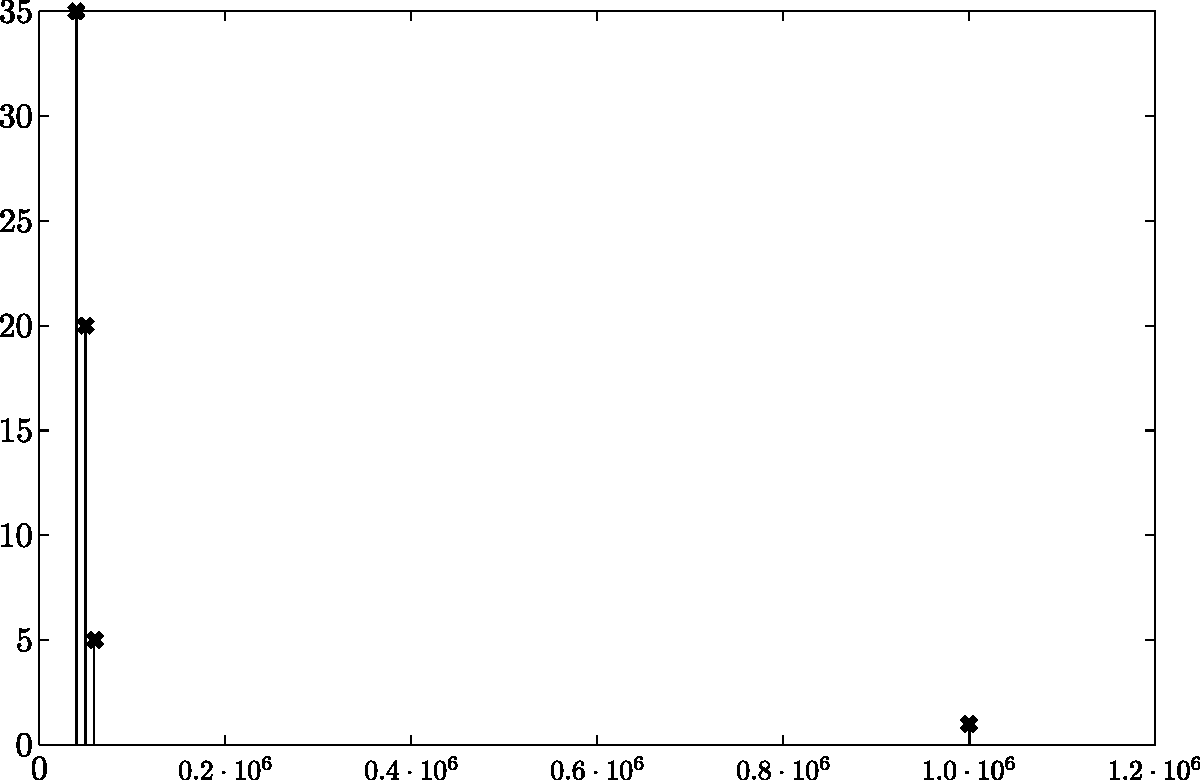
\includegraphics[width=0.5\textwidth]{figs/graph_salaires.pdf}
\caption{Nombre salariés en fonction du salaire.}\label{fig_salaires}
\end{center}
\end{figure}
ou d'un histogramme pour le temps d'exécution de l'application (voir Fig.~\ref{fig_exec}).
\begin{figure}[htp]
\begin{center}
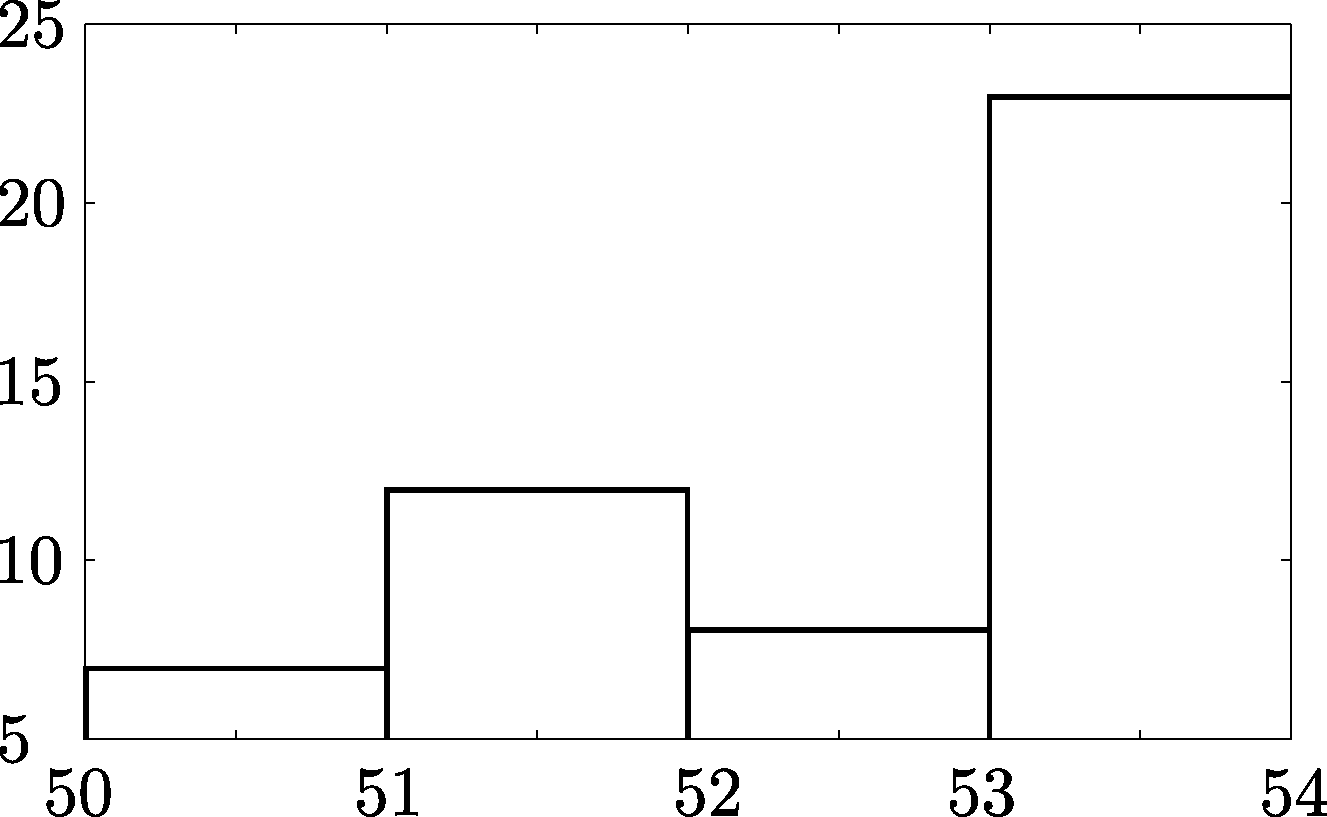
\includegraphics[width=0.5\textwidth]{figs/graph_exec.pdf}
\caption{Nombre d'exécutions en fonction du temps d'exécution.}\label{fig_exec}
\end{center}
\end{figure}

\subsection{Fréquences}

Plutôt que de faire apparaître le nombre d'individus d'une population 
possédant un caractère, il peut être plus intéressant et parlant de faire intervenir 
la \textit{fréquence} ou le nombre relatif à la place. En effet, la fréquence donne 
immédiatement la proportion d'individu plutôt qu'un nombre absolu qui n'est pas forcément 
très interprétable tout seul. 

La population totale, $n$, est donnée par
\begin{equation}
 n=\sum_{i=0}^{k-1}n_i.
\end{equation}
On peut donc définir la fréquence d'un caractère $i$, $f_i$ comme
\begin{equation}
 f_i=\frac{n_i}{n}.
\end{equation}
\begin{exemples}{Fréquence}

Les tableaux de fréquence des deux exemples précédents sont donnés par
 \begin{enumerate}
  \item Cas discret: la population totale est de 
  \begin{equation}
%    n=40'000+50'000+60'000+1'000'000=1'150'000.
   n=35+20+5+1=61.
  \end{equation}
  \begin{table}[htp]
  \begin{center}
  \begin{tabular}{|c|c|c|}
  \hline
  Salaire & Nombre de salariés & Fréquence\\
  \hline\hline
  40000 & 35 & $35/61\cong0.573770$\\
  \hline
  50000 & 20 & $20/61\cong0.327869$\\
  \hline
  60000 & 5 & $5/61\cong0.081967$ \\
  \hline
  1000000 & 1 & $1/61\cong0.19568$ \\
  \hline
  \end{tabular}
  \end{center}
  \caption{Tableau des salaires, du nombre de salariés et la fréquence.}
  \end{table}

  \item Cas continu: la population totale est de 
  \begin{equation}
   n=7+12+8+23=50.
  \end{equation}
  Le tableau \ref{table_exec_freq} affiche les différentes fréquences des temps d'exécution.
  \begin{table}[htp]
\begin{center}
\begin{tabular}{|c|c|c|}
\hline
 Temps d'exécution & Nombre & Fréquence \\
 \hline\hline
 [50,51) & 7 & $7/50=0.14$\\
 \hline
 [51,52) & 12 & $12/50=0.24$ \\
 \hline
 [52,53) & 8 & $8/50=0.16$ \\
 \hline
 [53,54) & 23 & $23/50=0.46$ \\
 \hline
\end{tabular}
\end{center}
\caption{Tableau des temps d'exécution et la fréquence des temps d'exécution.}\label{table_exec_freq}
\end{table}

 \end{enumerate}
\end{exemples}
La fréquence possède un certain nombre de propriétés que nous retrouverons 
dans les sections suivantes qui sont assez intuitives
\begin{proprietes}{Propriétés de la fréquence}
 \begin{enumerate}
  \item Les fréquences sont toujours dans l'intervalle $[0,1]$
  \begin{equation}
    0\leq f_i\leq 1.
  \end{equation}
  \item La somme de toutes les fréquences donne toujours $1$
  \begin{equation}
  \sum_{i=0}^{k-1} f_i = 1.
  \end{equation}

 \end{enumerate}

\end{proprietes}
Relié avec la propriété $2$ ci-dessus, il peut également être intéressant d'obtenir la
\textit{fréquence cumulée}, notée $F(x)$, d'un caractère qui se définit comme la fréquence des individus 
qui présentent une valeur de caractère $x_i\leq x$. Les tableaux correspondants aux tableaux 
\ref{table_salaires} et \ref{table_exec} (voir Tabls. \ref{table_salaires_freqcum} et \ref{table_exec_freqcum})
  \begin{table}[htp]
  \begin{center}
  \begin{tabular}{|c|c|c|c|}
  \hline
  Salaire & Nombre de salariés & Fréquence & Fréquence cumulée\\
  \hline\hline
  40000 & 35 & $35/61\cong0.573770$ & $35/61\cong0.573770$\\
  \hline
  50000 & 20 & $20/61\cong0.327869$ & $(20+35)/61\cong0.90164$\\
  \hline
  60000 & 5 & $5/61\cong0.081967$ & $(20+35+5)/61\cong0.98361$\\
  \hline
  1000000 & 1 & $1/61\cong0.19568$ & $(20+35+5+1)/61=1$\\
  \hline
  \end{tabular}
  \end{center}
  \caption{Tableau des salaires, du nombre de salariés, et la fréquence et fréquence cumulée des salaires.}\label{table_salaires_freqcum}
  \end{table}
  
  \begin{table}[htp]
\begin{center}
\begin{tabular}{|c|c|c|c|}
\hline
 Temps d'exécution & Nombre & Fréquence & Fréquence cumulée \\
 \hline\hline
 [50,51) & 7 & $7/50=0.14$ & $7/50=0.14$ \\
 \hline
 [51,52) & 12 & $12/50=0.24$ & $(7+12)/50=0.38$  \\
 \hline
 [52,53) & 8 & $8/50=0.16$ & $(7+12+8)/50=0.54$  \\
 \hline
 [53,54) & 23 & $23/50=0.46$ & $(7+12+8+23)/50=1$  \\
 \hline
\end{tabular}
\end{center}
\caption{Tableau des temps d'exécution et la fréquence et fréquences cumulées des temps d'exécution.}\label{table_exec_freqcum}
\end{table}
\begin{exercices}{Fréquence cumulée}
\begin{enumerate}
 \item Tracer les graphes de la fréquence cumulée pour les deux exemples que nous avons vus.
 \item Que pouvons-nous déduire de la forme de la fonction (croissance, valeur maximale)?
\end{enumerate}

 
\end{exercices}


\subsection{Mesures de tendance centrale}

Jusqu'ici le nombre de valeurs étudiées était limité et il est assez simple d'avoir 
une vue d'ensemble de la distribution des valeurs des caractères de notre population.
Il est plus aisé d'utiliser une nombre de valeurs beaucoup plus restreint permettant
de résumer les différents caractères et nous allons en voir deux différents qui nous donne une tendance dite centrale:
la moyenne, la médiane.

La \textit{moyenne}, notée $\bar{x}$ d'un jeu de données s'obtient par la formule suivante
\begin{equation}
 \bar{x}=\frac{1}{n}\sum_{i=0}^{k-1}x_i\cdot n_i.
\end{equation}
La moyenne peut également être calculée via les fréquences
\begin{equation}
 \bar{x}=\sum_{i=0}^{k-1}f_i\cdot x_i.
\end{equation}
\begin{exercices}{Propriétés de la moyenne}
\begin{enumerate}
 \item Démontrer la relation précédente.
 \item Démontrer que la moyenne des écart $x_i-\bar{x}$ est nulle.
\end{enumerate}
\end{exercices}

\begin{exemple}{Moyenne}

Pour l'exemple des salaires la moyenne est donnée par
\begin{equation}
 \bar{x}_{\textrm{salaire}}=\frac{35\cdot40000+20\cdot50000+5\cdot60000+1\cdot1000000}{61}=60656.
\end{equation}
\end{exemple}
On remarque ici que la moyenne des salaires donne une impression erronée de la situation car elle est très sensible aux valeurs extrême de la distribution.
En effet, tous les salaires à l'exception d'un sont inférieurs à la moyenne. En effet, si on retire le salaire d'un million de notre ensemble de valeurs, 
la moyenne de l'échantillon restant devient
\begin{equation}
 \bar{x}_{\textrm{salaire}}=\frac{35\cdot40000+20\cdot50000+5\cdot60000}{60}=45000.
\end{equation}
La différence est de l'ordre de $25\%$ par rapport aux $60'000$ CHF obtenus avec toute la population.
Il est donc nécessaire d'utiliser une autre mesure pour illustrer mieux le salaire caractéristique de notre population.
De façon plus générale la moyenne est peu robuste à des valeurs extrêmes dans l'étude d'échantillon.

Une mesure qui est plus parlante est la \textit{médiane}, notée $\tilde{x}$. La médiane se définit comme la valeur $\tilde{x}$ qui est telle que
la moitié des individus de la population sont ont un $x_i\leq \tilde{x}$ et le reste est telle que $x_i\geq\tilde{x}$.

Pour l'exemple des salaires le salaire médian est de $40000 CHF$, ce qui reflète beaucoup mieux la distribution des salaire de notre population.
\begin{exercice}{Moyenne, médiane}

 Calculer la moyenne et la médiane pour l'exemple du temps d'exécution (prendre la borne inférieure des intervalles pour chaque temps 
 d'exécution\footnote{Il y a 7 temps de 50s, 12 de 51s, 8 de 52s et 23 de 53s.}).
\end{exercice}


\subsection{Mesures de dispersion}

Nous avons vu deux mesures donnant une tendance générale des caractères d'une population. Hors cette valeur ne nous dit absolument rien
sur la manière dont ces caractères sont distribués. Sont-ils proches de la moyenne ou de la médiane? Ou en sont-ils au contraire éloignés?
Nous allons voir deux mesures différentes dans cette sous-section: la variance (écart-type), et l'intervalle inter-quartile.

Nous cherchons d'abord à calculer la moyenne des écarts à la moyenne. 
Hors, comme on l'a vu dans la sous-section précédente l'écart à la moyenne $x_i-\bar{x}$ est nul en moyenne. Cette grandeurs ne nous apprend rien. 
On peut donc s'intéresser plutôt à la moyenne de l'écart quadratique $(x_i-\bar{x})^2$ qui est une quantité toujours positive et donc la moyenne sera 
de cette écart quadratique aura toujours une valeurs qui sera positive ou nulle (elle sera nulle uniquement si 
$x_i-\bar{x}=0,\forall i$)\footnote{on pourrait aussi étudier la moyenne de $|x_i-\bar{x}|$, mais cela est moins pratique à étudier théoriquement.}.
On définit donc la \textit{variance}, $v$, comme étant la moyenne des écarts quadratiques
\begin{equation}
 v=\frac{1}{n}\sum_{i=0}^{k-1}n_i(x_i-\bar{x})^2.
\end{equation}
Si on considère plutôt la racine carrée de la variance, on obtient \textit{l'écart-type}
\begin{equation}
 s=\sqrt{v}.
\end{equation}
\begin{exercices}{Variance, écart-type}

Démontrer les relations suivantes
 \begin{enumerate}
  \item On peut également calculer la variance avec la fréquence
  \begin{equation}
   v=\sum_{i=0}^{k-1}f_i(x_i-\bar{x})^2.
  \end{equation}
  \item On peut également calculer la variance à l'aide de la formule suivante
  \begin{equation}
   v=\frac{1}{n}\left(\sum_{i=0}^{k-1}n_ix_i^2\right)-\bar{x}^2.
  \end{equation}
 \end{enumerate}
\end{exercices}
Pour l'exemple du salaire on obtient pour la variance
\begin{align}
 v&=\frac{1}{61}\left(35\cdot(40000-60656)^2+35\cdot(50000-60656)^2\right.\nonumber\\
 &\quad\quad\left.+35\cdot(60000-60656)^2+35\cdot(1000000-60656)^2\right)\nonumber\\
 &=1.4747\cdot 10^{10},
\end{align}
et l'écart-type
\begin{equation}
 s=\sqrt{v}=121440.
\end{equation}
\begin{exercice}{Variance, écart-type}

Calculer la variance et l'écart type à partir des valeurs du benchmark de l'application.
\end{exercice}

Encore une fois on constate que la valeur de l'écart-type des salaires est très dépendante de la valeur extrême de la distribution (1000000 CHF). 
Si on l'enlève la valeur de l'écart type est de $s=6455$ (un facteur 20 plus petit que la valeur sur la population complète).

Comme pour la moyenne et la médiane nous pouvons définir des valeurs plus représentatives. A partir de la fréquence cumulée, $F$,
on peut définir deux grandeurs, $Q_i\in\{x_i\}_{i=0}^{k-1}$ et $\alpha_i\in[0,1]$ telles que
\begin{equation}
 F(Q_i)=\alpha_i.
\end{equation}
En d'autres termes $Q_i$ est la valeur pour laquelle la fréquence cumulée vaut $\alpha_i$. $Q_i$ correspond donc au nombre d'individus dont la fréquence cumulée est de $\alpha_i$. 
En particulier si $\alpha_i=1/2$, alors $Q_i=\tilde{x}$ ($Q_i$ est la médiane). Il est commun d'avoir $Q_i\in[0.25,0.5,0.75]$, on parle alors de quartiles. Avec $Q_1=0.25$ et $Q_3=0.75$, 
le nombre d'individus entre $0.25$ et $0.75$ est donné par
\begin{equation}
 \frac{Q_3-Q_1}{2}.
\end{equation}
Cette valeurs est appelée l'intervalle semi-inter-quartile.
\begin{exercice}{Semi-inter quartile}

Calculer les intervalles semi-inter-quartiles des exemples que nous avons vus plus tôt dans le cours.
 
\end{exercice}

\section{Exemple du jeu de dé}

On considère un dé à 6 faces. Le lancer de dé est une \textit{expérience aléatoire}, car
on ne peut dire quel sera le résultat avant d'avoir effectué l'expérience. 

Avant de commencer à étudier les probabilités du lancer de dé, et les questions qu'on peut se poser, faisons d'abord un peu de vocabulaire
qui sera utile pour la suite.

\begin{definition}\hfill\break
 

\begin{itemize}
\item[$\bullet$] L'ensemble des résultats possibles du lancer de dé est $\Omega=\{1,2,3,4,5,6\}$ et cet ensemble est appelé l'\textit{univers} du lancer de dé.

\item[$\bullet$] Chaque résultat possible du lancer de dé ($1$, $2$, etc), noté $\omega\in\Omega$, est appelé une \textit{éventualité}.

\item[$\bullet$] Un ensemble de résultats possibles, par exemple tous les résultats pairs du lancer de dé $A=\{2, 4, 6\}\in\Omega$, s'appelle un \textit{événement}.
Un événement composé d'une seule éventualité est appelé \textit{événement élémentaire}.

\item[$\bullet$] On dit que l'événement $A$ est \textit{réalisé} si on obtient $2$, $4$, ou $6$ en lançant le dé.

\item[$\bullet$] \textit{L'événement certain} est l'univers en entier. On est certain de réaliser l'événement. 

\item[$\bullet$] \textit{L'événement impossible} est l'ensemble vide, $A=\emptyset$. Il correspondrait à l'événement obtenir $7$ ou plus en lançant un dé par exemple. 

\item[$\bullet$] Si $A$ est un événement, on note $p(A)$ la \textit{probabilité} que $A$ soit réalisé.

\end{itemize}
\end{definition}

Le calcul des \textit{probabilités} de réalisation de certains événement est reliée à la \textit{fréquence} 
que nous avons indroduit dans la section précédente. Soit un univers $\Omega$ et $A$, $B$ deux événements tels que $A\cap B=\emptyset$.
On effectue une $N$ expériences, donc $\Omega$ est réalisé $N$ fois. De plus on constate qu'on réalise $A$, $K$ fois et $B$, $M$ fois. 
On a donc les fréquences suivantes que $A$, $B$ et $\Omega$ se réalisent
\begin{align}
 f(A)&=\frac{K}{N},\\
 f(B)&=\frac{M}{N},\\
 f(\Omega)&=\frac{N}{N}=1,\\
 f(A\cap B)&=\frac{M+K}{N}=f(A)+f(B).
\end{align}
Les \textit{probabilités} de réalisation des événements ci-dessus peutvent être vues comme le passage à la limite
$N\rightarrow\infty$ tel que $p(A),p(B)\in\real$ et
\begin{align}
 p(A)&=\lim_{\substack{N\rightarrow\infty,\\ K/N<\infty}}\frac{K}{N},\\
 p(B)&=\lim_{\substack{N\rightarrow\infty,\\ M/N<\infty}}\frac{M}{N},\\
 p(\Omega)&=1,\\
 p(A\cap B)&=p(A)+p(B).
\end{align}

Si maintenant nous voulons connaître la probabilité de tirer $6$, ou encore la probabilité de réaliser $A=\{6\}$.  
Cela est assez intuitif pour le cas du dé. Nous avons $6$ éléments dans l'univers
du lancer de dé. La probabilité de réaliser $A=\{6\}$ est donc
\begin{equation}
 p(6)=\frac{1}{6}.
\end{equation}
Pour le cas du lancer de dé, on dit qu'on a un processus qui est \textit{équiprobable}. En effet,
la probabilité de réaliser chacun des événements élémentaires est la même. On a en effet la même probabilité de tirer 
$1$, $2$, $3$, $4$, $5$, ou $6$.

Si à présent, on se pose la question de la probabilité de réaliser un tirage pair, $A=\{2,4,6\}$, 
alors on trouve 
\begin{equation}
 p(\mbox{tirer un nombre pair})=\frac{1}{2}.
\end{equation}
De façon générale pour le lancer de dé, on a que la probabilité de réaliser l'événement $A$ est\footnote{De façon générale cela n'est pas vrai. Imaginons que nous
ayons un sac avec 3 boules: 2 noires et une blanche. La probabilité de réaliser $A$: tirer une boule noire ($p(A)=2/3$) ou $B$: tirer une boule blanche ($p(B)=1/3$) 
n'est pas donnné par $p(A)=\mbox{nombre d'éléments dans }A/\mbox{nombre total d'éléments}=1/2$, $p(B)=\mbox{nombre d'éléments dans }B/\mbox{nombre total d'éléments}=1/2$.}
\begin{equation}
p(A)=\frac{\mbox{nombre d'éléments dans }A}{\mbox{nombre d'éléments dans }\Omega}.
\end{equation}

Si maintenant, on veut savoir quelle est la probabilité de tirer n'importe quel élément dans l'univers, on a
\begin{equation}
p(\Omega)=\frac{\mbox{nombre d'éléments dans }\Omega}{\mbox{nombre d'éléments dans }\Omega}=1.
\end{equation}
De même la probabilité de réaliser l'événement impossible est de 
\begin{equation}
p(\emptyset)=\frac{\mbox{nombre d'éléments dans }\emptyset}{\mbox{nombre d'éléments dans }\Omega}=0.
\end{equation}
On voit ici une propriété fondamentale des probabilités qui est que $0\leq p(A)\leq 1,\ \forall A$.

La probabilité de ne pas tirer un 6 donc de réaliser l'événement $\bar A=\{1,2,3,4,5\}$ est donné par 
$1$ moins la probabilité de réaliser $A=\{6\}$, il vient
\begin{equation}
 p(\bar A)=1-p(A)=\frac{5}{6}.
\end{equation}
De même la probabilité de tirer un nombre impair, est donnée par $1$ moins la probabilité de réaliser 
l'événement pair
\begin{equation}
 p(\{1,3,5\})=1-p(\{2,4,6\})=\frac{1}{2}.
\end{equation}


\subsection{Evénements disjoints}\label{subsec_disjoints}
Considérons maintenant deux événements, $A=\{1,2\}$ et $B=\{3,4,5\}$. 
Comme $A$ et $B$ n'ont pas d'éléments en commun, on dit que c'est deux événements \textit{disjoints}. 
Les probabilités de réalisation de ces événements sont donc
\begin{align}
 p(A)&=\frac{2}{6}=\frac{1}{3},\\
 p(B)&=\frac{3}{6}=\frac{1}{2}.
\end{align}
On va se poser deux questions à présent
\begin{enumerate}
 \item On cherche à savoir quelle est la probabilité de réaliser $A$ ou de réaliser $B$, donc de tirer 
 un dé dont le résultat sera dans l'ensemble $C=A\cup B=\{1,2,3,4,5\}$. Le résultat est
 \begin{equation}
 p(C)=\frac{5}{6}.
 \end{equation}
 Une coincidence intéressante (qui n'est en fait pas une coincidence) est que
 \begin{equation}
 p(C)=p(A)+p(B)=\frac{1}{3}+\frac{1}{2}=\frac{5}{6}.
 \end{equation}
 \item On cherche à savoir quelle est la probabilité de réaliser $A$ et réaliser $B$ en même temps,
 donc de tirer un dé qui sera dans l'ensemble $C=A\cap B=\emptyset$. Ici on a déjà vu 
 que la probabilité $p(\emptyset)=0$.
\end{enumerate}
On voit donc que si des événements sont disjoints, alors la probabilité de réaliser 
l'un ou l'autre des événements est simplement la somme des probabilités de réaliser chacun des événements.
Inversément la probabilité de réaliser les deux événements en même temps est nulle.

Nous pouvons facilement décomposer $A$ en deux sous événements élémentaires, $A=\{1\}\cup \{2\}$.
On a donc une autre façon de calculer $p(A)$
\begin{equation}
p(A)=p(\{1\})+p(\{2\})=\frac{1}{6}+\frac{1}{6}=\frac{2}{6}=\frac{1}{3}.
\end{equation}
On a donc que la probabilité de réaliser un événement est la somme des événements élémentaires qui le composent.

\subsection{Evénements complémentaires}
Considérons de nouveau l'événement $A=\{1,2\}$ et cette fois l'événement $B=\Omega\backslash \{1,2\}=\{3,4,5,6\}$. L'événement 
$B$ est appelé \textit{l'événement complémentaire} de $A$. Il est noté $B=\bar A$. Les probabilité de réaliser $A$ ou de réaliser
$\bar A$ est la même chose que de réaliser l'événement certain, car $A\cup \bar A=\Omega$. 
On vérifie aisément dans ce cas que 
\begin{equation}
 \Omega=\{1,2\}\cup\{3,4,5,6\}.
\end{equation}
On a donc 
\begin{equation}
 p(A\cup \bar A)=p(\Omega)=1.
\end{equation}
De plus de ce qu'on a vu précédemment,
on a que 
\begin{equation}
p(A\cup \bar A)=p(A)+p(\bar A).
\end{equation}
En combinant ces deux derniers résultats, il vient que
\begin{equation}
p(A)+p(\bar A)=1.
\end{equation}
On en déduit que 
\begin{equation}
p(\bar A)=1-p(\bar A)=1-\frac{1}{3}=\frac{2}{3}.
\end{equation}
Dans ce cas on peut également calculer à priori $p(B)$
\begin{equation}
p(B)=\frac{\mbox{nombre d'éléments dans }B}{\mbox{nombre d'éléments dans }\Omega}=\frac{4}{6}=\frac{2}{3}.
\end{equation}
Ce résultat est très important car on calcule facilement $p(\bar A)$ si on connaît $p(A)$.



\subsection{Evénements non-disjoints}
Considérons de nouveau l'événement $A=\{1,2\}$ et cette fois $B=\{2,3,4,5\}$. Les probabilités de réaliser les événements
respectifs sont
\begin{align}
 p(A)&=\frac{1}{3},\\
 p(B)&=\frac{2}{3}.
\end{align}
La probabilité de réaliser $A$ et $B$ est maintenant la probabilité de réaliser $C=A\cap B=\{2\}$ 
\begin{equation}
 p(C)=\frac{1}{6}.
\end{equation}
Si on cherche à présent la probabilité de réaliser $A$ ou $B$, $D=A\cup B=\{1,2,3,4,5\}$, on voit aisément que 
\begin{equation}
 p(D)=\frac{5}{6}.
\end{equation}
Comme $A$ et $B$ ne sont pas disjoints ont constate 
\begin{equation}
 \frac{5}{6}=p(D)\neq p(A)+p(B)=1.
\end{equation}
L'inégalité est dûe au fait que dans le cas où on fait la somme $p(A)+p(B)$ on compte à double la probabilité de tirer l'éventualité $2$,
qui est l'intersection de $A$ et de $B$. Afin de corriger donc le calcul de $p(D)$ à partir de la somme $p(A)+p(B)$ il suffit d'enlever 
la probabilité de tirer l'intersection $C$. On a donc
\begin{equation}
 \frac{5}{6}=p(D)= p(A)+p(B)-p(C)=1-\frac{1}{6}=\frac{5}{6}.
\end{equation}
De façon complètement générale, on a la relation suivante pour calculer la probabilité de réaliser l'union de deux événement $A$ et $B$
\begin{equation}
 p(A\cup B)=p(A)+p(B)-p(A\cap B).
\end{equation}
Il en suit immédiatement que si $A\cap B=\emptyset$, alors
\begin{equation}
 p(A\cup B)=p(A)+p(B)-p(A\cap B)=p(A)+p(B)-p(\emptyset)=p(A)+p(B).
\end{equation}

\subsection{Axiomes des probabilités}
Tous ces concepts que nous avons vus précédemments peuvent être vus comme la conséquences des trois axiomes des probabilités
suivants
\begin{definition}{Axiomes  des probabilités}
Soit $\Omega$ un univers. La probabilité de réaliser un événement $A\subseteq\Omega$ est une fonction $p(A)$ qui associe à tout 
événement de $A$ un nombre réel, qui satisfait les 3 axiomes suivants
\begin{enumerate}
 \item Une probabilité est TOUJOURS positive
 \begin{equation}
  p(A)\geq 0.
 \end{equation}

 \item La probabilité de l'événement certain vaut 1
 \begin{equation}
  p(\Omega)=1.
 \end{equation}
 \item Soit $B\subseteq\Omega$. Si $A\cap B=\emptyset$, alors 
 \begin{equation}
 p(A\cup B)=p(A)+p(B). 
 \end{equation}
 La probabilité de réalisation de deux évéenements incompatibles est égale à la somme de réalisation
 de chacun d'entre eux.
\end{enumerate}
\end{definition}

De ces axiomes découlent tout un tas de théorèmes
\begin{theoreme}
Pour $A,B\subseteq\Omega$ et $\Omega$ un univers et $p$ une probabilité.
\begin{enumerate}
 \item $p(B\cap\bar A)=p(B)-p(B\cap A).$
 \item $p(\emptyset)=0.$
 \item $p(\bar A)=1-p(A).$
 \item $p(A\cup B)=p(A)+p(B)-p(A\cap B).$
 \item $p(\bar A\cap \bar B)=1-p(A\cup B).$
 \item Si $A$ et $B$ sont disjoints, alors $p(A\cup B)=p(A)+p(B).$ 
 \item Si $A\subseteq B$, alors $p(B\cap \bar A)=p(B)-p(A).$ 
 \item Si $A\subseteq B$, alors $p(A)\leq p(B).$ 
 \item $\forall A$, $0\leq p(A)\leq 1.$ 
\end{enumerate}

 
\end{theoreme}

\subsection{Probabilités conditionnelles}

Imaginons à présent que nous ayons une information supplémentaire lorsque nous lançons notre dé. 
Supposons par exemple que nous sachions lorsque nous lançons le dé que le résultat est pair. A partir de là
la probabilité de tirer un $6$ est de 
\begin{equation}
p(6\mbox{ sachant que le résultat du lancer est un nombre pair})=1/3,
\end{equation}
alors que sans l'information sur la parité nous aurions eu $p(6)=1/6$.

Lorsque nous rajoutons comme condition la réalisation préalable d'un événement $B$ à la réalisation d'un événement $A$,
nous parlons de probabilité conditionnelle, notée $P(A|B)$ (probabilité conditionnelle de $A$ sachant que $B$ s'est produit).

Essayons à présent de voir comment nous pouvons calculer de façon générale les probabilités conditionnelles avec notre exemple ci-dessus.
Nous avons donc que nous cherchons à calculer $p(A|B)=p(6|{2,4,6})$. Nous avons dans ce cas que $p(A)=1/6$, $p(B)=1/2$ et $p(A\cap B)=p(6)=1/6$.
Par ailleurs, nous pouvons remarquer que 
\begin{equation}
 p(A|B)=\frac{1}{3}=\frac{p(A\cap B)}{p(B)}=\frac{\frac{1}{6}}{\frac{1}{2}}.
\end{equation}
Nous pouvons vérifier cette relation sur un exemple un peu plus compliqué. Soit $A={1,2,4}$ et $B={2,4,6}$. La probabilité conditionnelle
$p(A|B)$ revient au calcul de la probabilité de $p(A\cap B|B)=p({2,4}|{2,4,6})=2/3$. Avec notre formule, nous avons
$p(A\cap B)=1/3$ et $p(B)=1/2$. Il vient donc
\begin{equation}
 p(A|B)=\frac{p(A\cap B)}{p(B)}=\frac{2}{3}.
\end{equation}
Cette formule peut en fait être vue comme la définition de la probabilité conditionnelle. 
Si $p(B)\neq0$ alors on appelle probabilité conditionnelle le nombre $p(A|B)$, tel que
\begin{equation}
 p(A|B)=\frac{p(A\cap B)}{p(B)}.
\end{equation}

\begin{exercice}{Probabilités conditionnelles}

Sur une population de 1000 hommes qui naissent, 922 atteignent l'âge de 50 ans et 665 l'âge de 70 ans. 
\begin{enumerate}
\item Quelle est la probabilité qu'un homme qui vient de naître soit encore en vie à 50 ans?
\item Quelle est la probabilité qu'un homme qui vient de naître soit encore en vie à 70 ans?
\item Quelle est la probabilité qu'un homme de 50 ans soit encore en vie à 70?
\end{enumerate}
\end{exercice}



\subsection{Evénements indépendants}

Prenons maintenant le cas ``pathologique'' où nous cherchons la probabilité conditionnelle $p(A|B)$, mais où 
la réalisation de $B$ n'a aucune influence sur la réalisation de $A$. On a donc 
\begin{equation}
 p(A|B)=p(A).
\end{equation}
On a donc que 
\begin{equation}
 p(A|B)=\frac{p(A\cap B)}{p(B)}=p(A).
\end{equation}
On en déduit que 
\begin{equation}
p(A\cap B)=p(A)\cdot p(B).\label{eq_indep}
\end{equation}
Et donc on peut calculer $p(B|A)$
\begin{equation}
p(B|A)=\frac{p(A\cap B)}{p(A)}=\frac{p(A)\cdot p(B)}{p(A)}=p(B).
\end{equation}
On a donc que si $A$ ne dépend pas de $B$, alors la réciproque est vraie aussi.
Les événements qui satisfonts la propriété de l'équation \eqref{eq_indep} sont appelés
indépendants. Dans le cas contraire ils sont appelé dépendants.

Afin d'illustrer l'indépendance, prenons à nouveau le jet de dé. Supposons que nous effectuions
deux tirages de suite et que l'événement $A$ soit ``tirer un 6 au premier tirage'' et que l'événement $B$
soit ``tirer un $2$ au deuxième tirage''. On a que 
\begin{equation}
 p(A)=\frac{1}{6},\quad p(B)=\frac{1}{6},\quad p(A\cap B)=\frac{1}{36}.
\end{equation}
On a donc bien $p(A\cap B)=p(A)\cdot p(B)$ et donc les événements sont indépendants. 
Cela semble bien naturel étant donné que le premier tirage du dé ne va en rien influencer le résultat du deuxieme 
tirage. Tout comme un tirage de l'euromillions d'une semaine ne va pas influencer le résultat de celui de la semaine suivante.

\begin{exercice}{Evénements indépendants}
On jette une pièce de monnaie deux fois de suite. Les résultats possible pour chaque jet sont: $P$, ou $F$.
\begin{enumerate}
 \item Ecrivez l'univers des événements.
 \item Calculez les probabilités des événements $A$ ``face au premier jet'', $B$ ``pile au second jet''.
 \item Calculez la probabilité $p(A\cap B)$. 
 \item Est-ce que les jets sont indépendants?
\end{enumerate}
\end{exercice}


\subsection{Tirages multiples}

Jusqu'ici on a lancer le dé une fois et calculé la probabilité liée à ce lancer unique. 
A présent, on va tirer le dé plusieurs fois et calculer les probabilité d'obtenir des séquences 
de réalisations. Pour notre exemple on va prendre un cas où on tire le dé deux fois successivement.
Ce type de tirage est appelé \textit{tirage successif avec remise}, car les deux tirages sont 
successifs et indépendants entre eux (on va tirer deux fois le même dé). L'univers de 
cette expérience est la combinaison de tous les résultats obtenus avec chacun des dés
\begin{equation}
 \Omega=\{11,12,13,14,15,16,21,22,23,24,25,26,...,61,62,63,64,65,66\}.
\end{equation}
Il y a $6\times 6=6^2=36$ résultats possibles à ce tirage. Il faut noter ici que l'ordre dans lequel le tirage 
a lieu est important; le tirage $26$ est différent du tirage $62$. On verra par la suite des exemples ou cela n'est pas le cas.

On cherche à savoir quelle est la probabilité d'obtenir l'événement $A=\{26\}$.

Comme précédemment la probabilité de réaliser l'événement $A$ est le nombre d'éléments dans $A$ divisé par le nombre d'éléments dans $\Omega$.
La probabilité est donc immédiatement obtenue
\begin{equation}
 p(A)=\frac{1}{36}.
\end{equation}
Une autre façon de visualiser ce genre de réalisation est de l'écrire sous forme d'arbre
(voir la figure \ref{fig_arbre}).
\begin{figure}[htp]
\includegraphics[width=\textwidth]{figs/arbre.pdf}
\caption{Représentation du tirage $26$ sous forme d'arbre.}\label{fig_arbre}
\end{figure}
Comme pour le cas à un tirage, tout tirage successif de dés est équiprobable et la probabilité
de chaque tirage est de $1/36$.

Une autre façon de calculer la probabilité d'obtenir $A=\{26\}$ est de constater que la probabilié 
d'obtenir ce tirage succesif est la probabilité de tirer $2$, puis la probabilité de tirer $6$. La probabilité
de cet enchaînement est obtenu en multipliant les événements élémentaires
\begin{equation}
 p(\{26\})=p(\{2\})\cdot p(\{6\})=\frac{1}{6}\cdot\frac{1}{6}.
\end{equation}
\begin{figure}[htp]
\includegraphics[width=\textwidth]{figs/arbre2.pdf}
\caption{Représentation du tirage $26$ sous forme d'arbre avec les probabilités associées.}\label{fig_arbre2}
\end{figure}
Afin de calculer la probabilité du tirage $26$ il suffit de suivre le chemin menant de la racine à la feuille correspondante
et de multiplier les probabilités inscrites sur chacune des branches.

Si à présent, nous voulons savoir quelle est la probabilité de tirer un $2$ ou un $4$ avec le premier dé et un nombre pair avec le second,
on a trois façons de calculer le résultat. La façon compliquée, où on compte toutes les possibilités. L'événement 
précédent s'écrit
\begin{equation}
 A=\{22,24,26,42,44,46\}.
\end{equation}
On a donc que $p(A)$ est donné par
\begin{equation}
 p(A)=\frac{\mbox{nombre d'éléments dans }A}{\mbox{nombre d'éléments dans }\Omega}=\frac{6}{36}=\frac{1}{6}.
\end{equation}
L'autre façon (plus simple) est d'utiliser la propriété du produit des probabilité. Nous savons que la probabilité de tirer un 
$2$ ou un $4$ avec le premier dé est de $1/3$, puis la probabilité de tirer un nombre pair avec le deuxième est de 
$1/2$. On a donc finalement que
\begin{equation}
 p(A)=\frac{1}{3}\cdot\frac{1}{2}=\frac{1}{6}.
\end{equation}
Finalement, on peut aussi utiliser la représentation sous forme d'arbre
où on somme simplement les probabilités de chacun des éléments de $A$
(voir figure \ref{fig_arbre3}).
\begin{figure}[htp]
\includegraphics[width=\textwidth]{figs/arbre3.pdf}
\caption{Représentation de l'événement $A=\{22,24,26,42,44,46\}$ sous forme d'arbre avec les probabilités associées.
Toutes les probabilités et tirages possibles associés aux branches ne sont pas affichées pour simplifier
l'affichage.}\label{fig_arbre3}
\end{figure}
Comme vu dans la section \ref{subsec_disjoints}, il suffit de prendre la somme des 
probabilités des événements élémentaires
\begin{align}
 p(A)&=p(\{22\})+p(\{24\})+p(\{26\})+p(\{42\})+p(\{44\})+p(\{46\})\nonumber\\
     &=\frac{1}{36}+\frac{1}{36}+\frac{1}{36}+\frac{1}{36}+\frac{1}{36}+\frac{1}{36}\nonumber\\
     &=\frac{6}{36}=\frac{1}{6}.
\end{align}

Si à présent l'ordre dans lequel les dés sont tirés n'a plus d'importance le calcul de probabilités change un peu.
On désire savoir quelle est la probabilité d'obtenir $26$ dans un ordre arbitraire. On peut donc obtenir
cette combinaison en tirant $26$ ou en tirant $62$. On a donc $A=\{26,62\}$. La probabilité de réaliser $A$
est donc
\begin{equation}
 p(A)=\frac{2}{36}=\frac{1}{18}.
\end{equation}
On peut calculer cette probabilité de nouveau avec l'arbre ou en comptant. Une façon de nouveau plus simple
dans bien des cas est d'utiliser les produits de probabilités. La probabilité de tirer
$26$ ou $62$ est la probabilité de tirer d'abord $2$ ou $6$, puis de tirer le nombre restant ($2$ si on a d'abord tiré $6$
ou $6$ si on a d'abord tiré $2$). La probabilité de tirer $2$ ou $6$ est de $1/3$, puis la probabilité de tirer
le nombre restant est de $1/6$. On a donc que
\begin{equation}
 p(A)=\frac{1}{3}\cdot \frac{1}{6}=\frac{1}{18}.
\end{equation}

\begin{exercices}
\hfill\break
 \begin{enumerate}
  \item Calculer la probabilité d'obtenir $2$ comme la somme des deux nombres tirés par deux dés.
  \item Calculer la probabilité d'obtenir $3,4,5,6,7,8,9,10,11,12$ comme la somme des deux nombres tirés par deux dés.
  \item Calculer la probabilité d'obtenir $7$ comme la somme des deux nombres tirés par deux dés.
  \item Calculer la probabilité d'obtenir $6$ soit avec 1 soit avec 2 dés.
  \item Déterminer le nombre de combinaisons possibles avec 3, 4, 5 dés. Pouvez vous généraliser à $n$ dés?
  \item Soit un tirage aléatoire offrant 2 possibilité (pile ou face par exemple). Quel est le nombre de combinaisons possibles 
  si on tire $n$ fois? Pouvez-vous généraliser pour un tirage aléatoire offrant $m$ possibilités qu'on tire $n$ fois?
 \end{enumerate}

\end{exercices}

\subsection{La distribution multinomiale}

Plus nous allon rajouter des tirages successifs plus il va être compliqué de calculer les probabilités 
de tirer une certaine combinaison de nombres. Il existe néanmoins une formule qui généralise les tirages successifs avec
remise. Prenons le cas où nous avons un dé qui ne donne pas chaque nombre de façon équiprobable, mais avec probabilité $\{p_i\}_{i=1}^6$.
Nous souhaitons savoir quelle est la probabilité de tirer deux fois le 1 et une fois le 2 lors de trois tirages successifs. 

Dans ce tirage l'ordre dans lequel sont obtenus ces tirages ne sont pas importants. Il y a donc les tirages possibles qui sont
admissibles
\begin{equation}
 [112]=\{112, 121, 211\}.
\end{equation}
On a donc que la probabilité associée est de
\begin{equation}
 p([112])=p(112)+p(121)+p(211).
\end{equation}
Ces trois probabilités sont données par
\begin{align}
 p(112)&=p_1\cdot p_1\cdot p_2=p_1^2\cdot p_2,\\
 p(121)&=p_1\cdot p_2\cdot p_1=p_1^2\cdot p_2,\\
 p(211)&=p_2\cdot p_1\cdot p_1=p_1^2\cdot p_2.
\end{align}
Les tirages étant indépendants (avec remise) on a que la probabilité de tirer $1$ ou $2$ est indépendante 
du moment où ils sont tirés et donc ces trois probabilités sont égales.

Finalement la probabilité de tirer deux 1 et un 2 est de
\begin{equation}
 p([112])=p(112)+p(121)+p(211)=3\cdot p_1^2\cdot p_2.
\end{equation}
Si à parésent nous considérons la probabilité de tirer $[1123]$ en 4 tirages. Les torages possibles sont
\begin{equation}
 [1123]=\{1123, 1132, 1213, 1231, 1312, 1321, 2113, 2131, 2311, 3112, 3121, 3211\}.
\end{equation}
Il y a donc 12 tirages possibles pour cette combinaison. De plus les tirages étant indépendants
on a que toutes ces combinaisons sont équiprobables avec probabilité
\begin{equation}
 p(1123)=p_1^2p_2p_3.
\end{equation}
Finalement on a 
\begin{equation}
 p([1123])=12 p_1^2p_2p_3.
\end{equation}
Si nous définissons $n_i$ le nombre de fois où on obtient le résultat $i$ et qu'on cherche la probabilité de réaliser le tirage $[n_1,n_2,...,n_k]$,
on constate que la probabilité de réaliser le tirage est proportionnelle à 
$p_1^{n_1}p_2^{n_2}\cdots p_6^{n_6}$. Il nous reste à déterminer le facteur multiplicatif venant devant. 
Pour le cas du tirage $1,1,2$, nous avons $[n_1n_2]$ avec $n_1=2$ et $n_2=1$ et le facteur devant le produit des probabilités est 
donné par $3$. Pour le tirage $1,1,2,3$ il est de $12$ et nous avons $n_1=2$, $n_2=1$, $n_3=1$. Nous pouvons écrire 
\begin{equation}
 3=\frac{3!}{1!2!}\mbox{ et } 12=\frac{4!}{1!1!2!}. 
\end{equation}
En fait on peut constater que
\begin{equation}
 \frac{n!}{n_1!n_2!\cdots n_6!},
\end{equation}
avec $n=\sum_{i=1}^6 n_i$. On a donc que 
\begin{equation}
 p([n_1,n_2,...,n_6])=\frac{n!}{n_1!\cdots n_6!}p_1^{n_1}\cdots p_6^{n_6}.
\end{equation}
De façon complètement générale ce genre de probabilité se calcule grâce à la \textit{distribution multinomiale}
\begin{equation}
 p([n_1,...,n_k])=\frac{n!}{n_1!\cdots n_k!}p_1^{n_1}\cdots p_k^{n_k}.
\end{equation}

\begin{exercices}
\hfill\break
  On lance un dé parfait 10 fois. Quelle est la probabilité d'obtenir:
 \begin{enumerate}
  \item 10 fois 6?
  \item 4 fois 3, 3 fois 2 et 3 fois 1?
  \item 2 fois 1, 2 fois 2, 2 fois 3, 1 fois 4, 1 fois 5, et 1 fois 6?
 \end{enumerate}

\end{exercices}

\section{Exemple du lotto}
Dans un lotto on a dans un sac un nombre de jetons numérotés, disons pour l'exemple entre 1 et 6, 
qui sont tirés successivement. Une fois un jeton tiré, il ne sera pas remis dans le sac. 
On appelle ce genre de tirage \textit{sans remise}. Contrairement au cas des dés vus dans 
la section précédente qui était `\textit{avec remise}.
On tire un nombre fixé de jetons, disons 3. On souhaite déterminer la probabilité d'obtenir
une suite donnée de 2 numéros, disons $25$. Disons que pour cet exemple l'ordre du tirage a de l'importance
(ce qui n'est pas le cas du lotto).

Afin de calculer cette probabilité le fait qu'on effectue un tirage avec remise est promordial.
En effet considérons le cas initial illustré dans la figure \ref{fig_loto}.
\begin{figure}[htp]
\includegraphics[height=1.8truecm]{figs/loto.pdf}
\caption{Les six numéros présents initialement dans le sac.}\label{fig_loto}
\end{figure}
Pendant le premier tirage, nous tirons le numéro 2 (voir figure \ref{fig_loto2}). Notons que le tirage du 2 a une probabilité $\frac{1}{6}$.
\begin{figure}[htp]
\includegraphics[height=1.8truecm]{figs/loto2.pdf}
\caption{Le numéro 2 est tiré lors du premier tirage.}\label{fig_loto2}
\end{figure}
Il est donc enlevé du sac et il nous reste uniquement 5 chiffres parmis lesquels choisir 
(les chiffres $1$, $3$, $4$, $5$, et $6$, comme dans la figure \ref{fig_loto3}).
\begin{figure}[htp]
\includegraphics[height=1.8truecm]{figs/loto3.pdf}
\caption{Il ne reste que 5 chiffres dans le sac.}\label{fig_loto3}
\end{figure}
Comme il ne nous reste que 5 chiffres, la probabilité de tirer un des nombres restant, 
disons le $5$, est de $\frac{1}{5}$ (voir la figure \ref{fig_loto4}). 
\begin{figure}[htp]
\includegraphics[height=1.8truecm]{figs/loto4.pdf}
\caption{Il ne reste que 5 chiffres dans le sac et nous tirons le 5.}\label{fig_loto4}
\end{figure}
Le 5 sera lui aussi retiré et il ne restera que 4 numéros dans le sac et ainsi de suite. 

On voit donc que la probabilité de tirer la suite ordonnée $25$ est de
\begin{equation}
 p(\{25\})=p(\{2\})\cdot p(\{5\})=\frac{1}{6}\cdot\frac{1}{5}=\frac{1}{30}.
\end{equation}
A présent, si nous considérons que l'ordre n'a pas d'importance, on a comme dans la section précédente
que l'événement qui nous intéresse est $A=\{25,52\}$. On peut donc décomposer 
ce cas en 2 et dire qu'on a dans un premier temps la probabilité de tirer $2$ ou $5$ parmis 
$6$ nombres, puis on a la probabilité de tirer le $5$ ou le $2$ (respectrivement si on a tiré $2$ ou $5$) parmis 5.
Les deux probabilité sont donc données respectivement par $p(\{2,5\})=\frac{2}{6}$ puis par $p(\{5,2\}\backslash \{2\mbox{ ou }5)=\frac{1}{5}$.

\begin{exercices}
\hfill\break
 \begin{enumerate}
  \item Le jeu Eruomillions consiste en un tirage de 5 numéros parmis 50 possible, puis par le tirage de 2 ``étoiles'' parmis 11 possibles.
  Déterminez la probabilité de trouver la bonne combinaison à un tirage.
  \item Le jeu du swiss lotto, consiste au tirage de 5 numéros parmis 42 possibles, puis au tirage d'un numéros parmis 6. Calculez la probabilité de 
  gagner au swiss lotto..
 \end{enumerate}
\end{exercices}

\section{Quelques exercices}
Afin de continuner avec ces concepts de tirages aléatoires avec ou sans remise
de suite ordonnées ou non, nous allons faire quelques exercices. Il peut se révéler utile de dessiner un arbre pour ces exercices.
\begin{enumerate}
 \item Dans une urne se trouvent 2 boules blanches et 3 boules noires. On tire successivement deux boules sans remise.
Calculer et comparer les probabilités des deux événements suivants
\begin{itemize}
 \item[$\bullet$] Tirer deux boules de même couleur.
 \item[$\bullet$] Tirer deux boules de couleurs différentes.
\end{itemize}
\item Une bille, lâchée en $O$ tombe dans l'une des trois boîtes $A$, $B$, ou $C$. A chaque bifurcation, la bille 
tombe à gauche avec la probabilité de 0.25 et à droite avec la probabilité de 0.75 (voir figure \ref{fig_bille})
\begin{figure}[htp]
\begin{center}
\includegraphics[height=2.8truecm]{figs/bille.pdf}
\end{center}
\caption{Une bille lâchée en $O$ tombe dans la boîte $A$, $B$, ou $C$.}\label{fig_bille}
\end{figure}
\begin{itemize}
 \item[$\bullet$] Calculer les probabilités $p(A)$, $p(B)$, $p(C)$ pour qu'une bille lâchée de O tombe respectivement 
dans la boîte $A$, $B$ ou $C$.
\item[$\bullet$] On lâche deux billes en $O$. Calculer la probabilité pour que les deux billes tombent dans la même boîte.
\item[$\bullet$] On lâche trois billes en $O$. Calculer la probabilité d'avoir une bille dans chaque boîte.
\item[$\bullet$] On lâche dix billes en $O$. Calculer la probabilité d'avoir au moins trois billes dans la boîte B.
\end{itemize}
\item A la naissance, la probabilité qu'un enfant soit un garçon
est de $p(G)=0.514$.
\begin{itemize}
 \item[$\bullet$] Calculer et la probabilité qu'un enfant soit une fille.
 \item[$\bullet$] On considère la naissance de deux enfants. Calculer et la probabilité que les deux enfants sooient de même sexe.
 \item[$\bullet$] On considère la naissance de deux enfants. Calculer et la probabilité que les deux enfants soient de sexes opposés.
\end{itemize}
\end{enumerate}

\section{Variables aléatoires}

Lors d'une expérience aléatoire, il est assez commun de relier chaque événement de l'univers, $A\in\Omega$, à un nombre réel, $X(A)\in\real$. 
Cette relation est définie par une fonction qui porte le nom de variable aléatoire et peut s'écrire mathématiquement sous la forme
\begin{equation}
 X:\Omega\rightarrow \real.
\end{equation}
Afin de mieux comprendre ce concept voyons quelques exemples
\begin{enumerate}
 \item[Le jeu de dé:] Lors d'un jet de dé unique l'univers est défini par $\Omega=\{1,2,3,4,5,6\}$. On peut de façon assez naturelle 
 définir notre variable aléatoire comme
 \begin{equation}
  X:i\rightarrow i.
 \end{equation}
 \item[Pile ou face:] Si nous lançons une pièce de monnaie les deux issues possibles sont pile $p$, ou face $f$ ($\Omega={p,f}$). 
 Nous pouvons définir la variable aléatoire $X$ comme
 \begin{equation}
  X:\left\{\begin{array}{l}
                p\rightarrow 0\\
                f\rightarrow 1
               \end{array}\right.
 \end{equation}
 \item[Pile ou face$^2$:] Si nous lançons une pièce de monnaie à deux reprises, les issues possibles sont $(p,p)$, 
 $(p,f)$, $(f,p)$, $(f,f)$. Nous pouvons définir la variable aléatoire $X$ comme
 \begin{equation}
  X:\left\{\begin{array}{l}
                (p,p)\rightarrow 0\\
                (p,f)\rightarrow 1\\
                (f,p)\rightarrow 1\\
                (f,f)\rightarrow 2
               \end{array}\right.
 \end{equation}
\end{enumerate}
Comme nous nous sommes posés la question de connaître la probabilité d'obtenir un certain résultat lors d'une expérience aléatoire, il en va de même 
avec la probabilité que la variable aléatoire $X$ prenne une valeur donnée, $\alpha\in\real$ ou prenne une valeur incluse dans un intervalle $I\subseteq\real$. 

Pour illustrer ce qui se passe, intéressons-nous au dernier exemple ci-dessus avec le double pile ou face. On se pose les questions suivantes
\begin{enumerate}
 \item Quelle est la probabilité que $X$ prenne la valeur $1$?
 \item Quelle est la probabilité que $X$ prenne une valeur incluse dans $I=[0.6,3]$?
 \item Quelle est la probabilité que $X$ prenne une valeur inférieure à $2$?
\end{enumerate}

Prenons ces trois questions une par une
\begin{enumerate}
 \item Les deux façons d'obtenir $X=1$ est d'avoir les tirages $(p,f)$ ou $(f,p)$, soit $A=\{(p,f), (f,p)\}$. Les probabilités de chacun 
 des événement de l'univerrs étants équiprobables on a 
 \begin{equation}
  p(X=1)=p(A)=1/2.
 \end{equation}
 \item Le seul événement donnant un $X$ qui n'est pas dans l'intervalle $J=[0.6,3]$ est $B=(p,p)$ ($X(B)=0$). On a donc que 
 \begin{equation}
p(0.6\leq X\leq 3)=p(\bar B)=1-p(B)=\frac{3}{4}.
 \end{equation}
 \item De façon similaire les trois énénements donnant $X<2$ sont dans $C=\{(p,p), (p,f), (f,p)\}$. On a donc
 \begin{equation}
  p(X<2)=p(C)=\frac{3}{4}.
 \end{equation}

\end{enumerate}
On constate au travers de ces trois exemples que la probabilité que la variable 
aléatoire $X$ prenne une valeur particulière $\alpha$ ou soit dans un intervalle $I$ 
est reliée à la probabilité d'obtenir un événement $D$ qui serait la préimage de $\alpha$ ou d'un intervalle $I$.
On peut noter dans le cas général qu'on a $D=X^{-1}(I)$.

\begin{definition}[Variable aléatoire] On dit que la fonction $X:\Omega\rightarrow\real$ est une \textit{variable aléatoire} si la 
préimage de $X$ sur tout intervale, $I\subseteq\real$, est un événement $A\in \Omega$. La probabilité que $X$ prenne une valeur 
dans l'intervalle $I$ est égale à la probabilité de réaliser l'événement $A$
\begin{equation}
 p(X\in I)=p(A).
\end{equation}
\end{definition}

\begin{definition}[Fonction de répartition] On dit que la fonction $F:\real\rightarrow\real$ est une \textit{fonction de répartition}
si $F(x)=p(X\leq x)$ pour tout $x\in\real$.
\end{definition}

Nous distinguons deux sortes de variables aléatoires différentes: les variables aléatoires discrètes et continues. Nous les discuterons brièvement dans les deux sous-sections suivantes.


\section{Nombres aléatoires}

Les nombres aléatoires, bien que pas directement reliés aux probabilités, sont utilisés dans un certain nombre de domaines
qui vont de la cryptographie aux simulations physiques. Nous allons voir une introduction simplifiée à la génération de nombres aléatoires
sur un ordinateur et les différentes problématiques reliées à leur génération.

Une très bonne référence concernant les nombre aléatoires est le site \break \texttt{http://www.random.org}.

\subsection{Générateurs algorithmiques: une introduction (très) générale}

Le but des générateurs de nombres aléatoires est de produire une suite de nombres entiers,
($n\in\natural$)
\begin{equation*}
 \{X_0,X_1,...,X_n\},
\end{equation*}
avec $X_i\in A$, où $A=[0,M]$, avec $m\in \natural$ (dans le cas de la fonction \texttt{rand()}
de $C$, $M$ est donné par la constante prédéfinie \texttt{RAND\_MAX} qui and certains cas est $2^{31}-1$). La probabilité 
de tirer chacun des nombres dans l'intervalle est égale. On dit que la distribution des nombres est uniforme.
De plus, les nombres tirés ne doivent pas dépendre de l'histoire des nombres tirés précédemment. 

Si on veut maintenant plutôt tirer des nombres réels uniformément distribués entre $[0,1]$, il suffit
de diviser les nombres $X_i$ par $m$ après chaque tirage. De façon similaire, si nous voulons 
tirer des nombres dans l'intervalle $[\alpha,\beta]$, on utilise la formule de remise à l'échelle suivante
\begin{equation}
 N_i=\alpha+(\beta-\alpha)X_i/m.
\end{equation}
Il faut remarquer que pour que cette formule puisse est utilisée il est nécessaire que $(\beta-\alpha)<M$.

Les transformations que je donne ici ne sont pas toujours celles implémentées. En effet,
il existe des transformations beaucoup plus efficaces d'un point de vue computationnel
pour changer l'intervalle des nombres aléatoires tirés.

Sans entrer dans les détails, la génération de nombres aléatoires n'ayant pas une distribution
uniforme s'obtient en effectuant une transformation un peu plus complexe que celle ci-dessus
en partant toujours de la suite de nombres aléatoires entiers.

Les nombres aléatoires produits de façon algorithmique (donc avec un ordinateur)
ne peuvent pas être vraiment aléatoire, car ils sont obtenus avec une machine 
déterministe (les opérations faites à l'aide d'un ordinateur sont par définition
reproductibles avec une chance d'erreur quasiment nulle). On parle donc de nombre pseudo-aléatoires.

Néanmoins, bien que ces chiffres ne soient pas vraiment aléatoires, ils peuvent 
être posséder des propriétés qui les rendent satisfaisants pour la plupart des applications. Cette suite de nombres doit avoir des propriétés particulières quand $n\rightarrow\infty$.
Sans entrer pour le moment trop dans les détails, on veut par exemple que 
la moyenne des nombres tirés soit $m/2$, que la corrélation entre des 
sous-suites de nombres doit être nulle, ou encore qu'il n'existe pas de séquence qui se 
répète (ou au moins que la période de répétition soit très très longue).
Néanmoins, il est assez compliqué de définir des tests
très robustes pour tester la qualité des nombres aléatoires algorithmiques.


\subsection{Les générateurs congruenciels linéaires}\label{sec_congr}

Pendant très longtemps, les générateurs de nombres aléatoires algorithmiques
ont été des générateurs congruenciels linéaires, dont la génération est 
donné par la formule suivante. Soit $X_i$ un nombre aléatoire,
alors le prochain nombre de la série est donné par
\begin{equation}
X_{i+1}=(aX_i+c)\mod m,
\end{equation}
où $a$, $c$ et $m$ sont des paramètres de notre générateur. 
On constate que la seule partie 
éventuellement aléatoire de n'importe quelle séquence est la valeur initiale 
de notre séquence $X_0$ (aussi appelée \textit{graine}). 
Tous les autres nombres obtenus sont déterministes. Pour chaque valeur de graine, 
on aura toujours la même séquence de nombre tirés.

Il est très important de noter que la qualité des nombres aléatoires obtenus
sont extrêmement dépendants des valeurs de $a$, $c$ et $m$ choisies (et des 
relations entre elles). Si par exemple, on choisit 
$a=1$, $c=1$, $m=10$ et $X_0=0$, on va avoir comme suite de nombre aléatoire
\begin{equation}
 \{0,1,2,3,4,5,6,7,8,9,0,1,2,3,...\},
\end{equation}
ce qui n'est pas très aléatoire vous en conviendrez... Il est donc très important
de tenter d'optimiser les valeur $a$, $c$ et $m$ pour
avoir des séquences aussi ``aléatoires'' que possible.

Une première chose à remarquer c'est que $m$ sera la valeur maximale de la période
de notre générateur de nombre aléatoire (la période est le nombre de tirage qu'il faudra
effectuer pour que la série se répète exactement).

Quelques paramètres utilisés dans des générateurs connus sont par exemple
\begin{itemize}
 \item[$\bullet$] la fonction \texttt{rand()} du langage $C$ 
 \begin{equation*}
  a=1103515245,\quad c=12345,\quad m=2^{32}.
 \end{equation*}
 \item[$\bullet$] la fonction \texttt{drand()} du langage $C$ 
 \begin{equation*}
  a=25214903917,\quad c=11,\quad m=2^{48}.
 \end{equation*}
 \item[$\bullet$] le générateur \texttt{RANDU} des ordinateurs IBM des années 1960
 \begin{equation*}
  a=65539,\quad c=0,\quad m=2^{32}.
 \end{equation*}
\end{itemize}

Ce genre de générateur de nombres aléatoires est très efficace d'un point de vue computationnel
mais la qualité des nombres aléatoires peut être insuffisante. Plusieurs améliorations
ont été proposées. Par exemple, pour chaque étape, on peut générer $k$ nombres aléatoires
avec un générateur congruentiel linéaire et combiner les nombres.

La méthode probablement la plus populaire consiste à utiliser 
des récurrences matricielles sur la représentation binaire des nombres.
Soit $\tilde X_i$ la représentation sur $k$ bits de $X_i$, alors 
$\tilde X_{i+1}$ est donné par
\begin{equation}
 \tilde X_{i+1}=A \tilde X_i \mod 2,
\end{equation}
où $A$ est une matrice $k\times k$. Ce genre de générateur a l'énorme
avantage d'être extrêmement efficace. Ils sont à la base de l'algorithme Mersenne Twister.
Ces générateurs ont généralement une période extrêmement longue (qui a la particularité d'être
un nombre premier de type Mersenne dont la forme est $m=2^l-1$, avec $l\in\natural$).

Bien que ne soyant pas parfaits ces générateurs ont le grand avantage d'être très rapides et peu
gourmands en ressources de calcul. La facilité de description et d'utilisation
de tels  générateurs, permet des tests très poussés quant à leur qualités et leurs limites
par la communauté scientifique. Finalement, les besoins de débuggage de codes,
la reproductibilité d'une série de nombres aléatoires
peut être d'un grand secours. 

\subsection{Les générateurs physiques}

Une autre façon de générer des nombres aléatoires, serait d'utiliser des phénomènes physiques
qui contiennent de façon inhérente des processus aléatoires. On peut imaginer 
lancer un dé ``à la main'', mesurer les émissions radioactives d'atomes (mesurer leur spin), 
etc... Ou encore effectuer des lancer de jeux aussi peu biaisés que possibles (roulette, dé, etc).

Néanmoins, cette façon de faire a un certain nombre de désavantages. Le premier
est que l'acquisition des données ``en temps réel'' de ces processus est en général plusieurs
ordres de grandeurs trop lente par rapport aux besoins pratiques. Par rapport à un générateur algorithmique
très peu coûteux, un dispositif ``physique'' peut être très coûteux en espèces sonnantes et trébuchantes.

Il a néanmoins été envisagé de stocker de très grandes quantités de nombres aléatoires
sur un support quelconque et de les fournir à l'utilisateur quand cela s'avère nécessaire.
Le problème principal qui a été révélé par cette façon de faire est que le processus de mesure
des différents processus est loin d'être parfait et engendre des biais importants 
dans la qualité des nombres obtenus ce qui les rend souvent en pratique moins bons que 
les nombres obtenus avec des générateurs de nombres pseudo-aléatoires...

\subsection{Comment décider si une suite de nombres pseudo-aléatoires peut 
être considérée comme aléatoire}

Cette question est extrêmement compliquée. Pour simplifier considérons le tirage de nombres 
entiers $X_i\in \{0,1\}$. Les tirages aléatoires sont uniformément distribués,
on a donc que $p(0)=p(1)=1/2$. Supposons qu'on obtient une suite de 10 nombres 
avec deux générateurs différents
\begin{align}
 X&=\{0,0,1,1,1,0,1,0,1,0\},\\
 Y&=\{0,0,0,0,0,0,0,0,0,0\}.
\end{align}
On voit que la suite $Y$ semble beaucoup moins aléatoire que la suite $X$. 
En effet, la probabilité de tirer 10 fois 0 en 10 tirages et de $p(Y)=1/2^{10}=1/1024$,
alors que la probabilité d'avoir autant de 0 que de 1 est de $p(X)=1/2$.
De façon générale on aimerait que la répartition soit $35\%$-$65\%$ avec une probabilité
de $90\%$.

Néanmoins, ce critère n'est pas suffisant. En effet la suite
\begin{equation}
 Z=\{0,1,0,1,0,1,0,1,0,1\},
\end{equation}
satisfait bien le critère ci-dessus. En revanche la probabilité de n'avoir pas deux tirages 
$0$ ou $1$ de suite est très faible (moins de $5\%$). 

De ces constatations on peut dire qu'un générateur de nombres pseudo-aléatoires est de bonne
qualité si les tirages qui sont effectués vérifient les propriétés du tirage 
avec une forte probabilité. On constate que cette définition est vague. En particulier
la définition de ``forte'' est pas très précise. Il faut cependant noter que
souvent nous sommes intéressés à des suites qui ont une longueur $n$. 
Donc pour $n\rightarrow\infty$ on va vouloir que les probabilités vont 
toutes tendre vers $1$. 

Néanmoins, il est certain qu'aucun générateur ne peut être parfait. En effet,
les nombres étant toujours représentés avec une précision finie, il est impossible
d'être capable de représenter exactement toutes les propriétés d'une série de nombre
vraiment aléatoires avec un générateur pseudo-aléatoire. On va donc plutôt
considérer une autre définition pour la qualité d'un générateur algorithmique.

Considérons une simulation nécessitant la génération de nombres aléatoires.
Un ``bon'' générateur de nombres pseudo-aléatoire produit une série de nombre
qui peut être utilisée en lieu et place de vrai nombres aléatoires sans que la simulation
n'en soit affectée. Par exemple, le calcul du nombre $\pi$ vu dans les exercices doit 
être trouvé avec la précision désirée avec le générateur de nombre pseudo-aléatoires pour que celui-ci 
soit considéré comme bon.

\subsection{Quelques règles générales}

La règle précédente bien que satisfaisante, n'est pas forcément simple à tester. En effet,
il ne permet pas de prévoir la qualité d'un générateur a priori. Il nous faut donc quelques 
qualités minimales pour les générateurs de nombres aléatoires.

\subsubsection{La périodicité}

Tout générateur de nombres pseudo-aléatoires va à un moment ou un autre devenir périodique (la séquence de nombres générés vont 
se répéter à l'infini). Notons la période du générateur aléatoire $T$. 
Il est évident que dès qu'on atteint un nombre de tirages équivalent à la période ($\card(X)\sim T$), on va avoir des nombres 
pseudo-aléatoires qui ne sont plus du tout satisfaisants. En fait on peut montrer que des problèmes apparaissent dès que
le nombre de tirages atteint un nombre équivalent à $T^{1/3}$. 
Une condition primordiale pour avoir un ``bon'' générateur de nombres pseudo-aléatoire est donc une période élevée.
Pour des générateurs aléatoires modernes, 
un période $T<2^{100}$ n'est pas considéré comme satisfaisant pour la plupart des applications.

Évidemment il est impossible de tester la périodicité de tels générateurs de façon 
expérimentale ($2^{100}\sim 10^{30}$). Cela ne peut se faire que par des études analytiques
approfondies. Comme expliqué dans la section \ref{sec_congr}
la période maximale d'un générateur congruentiel linéaire est $m$. Dans les 3 exemples
donnés la période est respectivement de $2^{32}$, $2^{48}$, ou $2^{32}$. Ils ne devraient donc
plus être utilisés dans des applications modernes. A titre de comparaison le générateur Mersenne Twister possède une période de $2^{19937}-1$.

Il est évident que la période à elle seule ne suffit pas à déterminer si un 
générateur de nombres pseudo-aléatoires est bon. En particulier on peut prendre un générateur congruentiel, où 
\begin{equation}
 X_{i+1}=(X_i+1)\mod m,
\end{equation}
avec $m$ aussi grand qu'on veut (disons $m=2^{2000}$ par exemple) mais la séquence de
nombres générés ne sera absolument pas aléatoire, étant donné qu'on aura
\begin{equation}
 X=\{0, 1, 2, 3, 4, 5, 6, ..., 2^{2000}-1, 0, 1, 2, ...\},
\end{equation}
si $X_0=0$. Cela pourrait ne pas être problématique en soit, si la séquence avec une graine $X_0=1$ n'était pas si similaire
\begin{equation}
 X=\{1, 2, 3, 4, 5, 6, ..., 2^{2000}-1, 0, 1, 2, ...\}.
\end{equation}
Il est donc nécessaire d'avoir d'autres critères que la seule période.
C'est le sujet de la sous-section suivante.

\subsubsection{La discrépance}

Afin d'éliminer les générateurs de nombres pseudo-aléatoires comme l'exemple qu'on 
vient de citer, il faut étudier la répartition des nombres. Sans tomber dans le cas pathologique de la section
précédente, on peut imaginer des nombres qui ont l'air aléatoires, mais qui ont un biais. 
Reprenons l'exemple du tirage entre $[0,1]$. Nous pouvons imaginer une suite très longue 
sans période avec des tirages aléatoires, mais avec beaucoup plus de 0 que de 1, ce qui évidemment serait problématique.

On doit donc trouver un moyen de tester la répartition des nombres de façon plus quantitative.
Une façon de le faire est de considérer l'ensemble des $k-$uplets de nombres définis par
\begin{equation}
 X^k=\{X_1,X_2, ..., X_k\},
\end{equation}
où $X_0$ est supposé tiré uniformément dans l'ensemble de départ (ici supposons que c'est $[0,1]$ à titre d'exemple).
En prenant toutes les graines existantes, on attend d'un bon générateur qu'il recouvre tout l'espace des résultats possibles
pour les $k-$uplets formés avec des nombres aléatoires dans $[0,1]^k$. En d'autres termes, il faut que des graines différentes
génèrent des $k-$uplets différents pour toutes valeurs de $k$. 

De nouveau ce genre de tests est très compliqué à tester expérimentalement pour $k$ de l'ordre de la période 
du générateur de nombres aléatoires. Des analyses théoriques sont dès lors primordiales, mais bien en dehors 
du champs de ce cours...

Il existe beaucoup d'autres tests possibles (il y a des recommandations sur le site \texttt{http://www.random.org} 
pour tester des nombres aléatoires. 

\end{document}
